\documentclass{article}

  % packages
    % basic stuff for rendering math
    \usepackage[letterpaper, top=1in, bottom=1in, left=1in, right=1in]{geometry}
    \usepackage[utf8]{inputenc}
    \usepackage[english]{babel}
    \usepackage{amsmath} 
    \usepackage{amssymb}

    % extra math symbols and utilities
    \usepackage{mathtools}        % for extra stuff like \coloneqq
    \usepackage{mathrsfs}         % for extra stuff like \mathsrc{}
    \usepackage{centernot}        % for the centernot arrow 
    \usepackage{bm}               % for better boldsymbol/mathbf 
    \usepackage{bbm}
    \usepackage{enumitem}         % better control over enumerate, itemize
    \usepackage{xr-hyper}
    \usepackage{hyperref}         % for hypertext linking
    \usepackage{fancyvrb}          % for better lstlisting environments
    \usepackage{newverbs}         % for texttt{}
    \usepackage{xcolor}           % for colored text 
    \usepackage{listings}         % to include code
    \usepackage{lstautogobble}    % helper package for code
    \usepackage{parcolumns}       % for side by side columns for two column code
    \usepackage{algorithm}
    \usepackage{algpseudocode}

    % page layout
    \usepackage{fancyhdr}         % for headers and footers 
    \usepackage{lastpage}         % to include last page number in footer 
    \usepackage{parskip}          % for no indentation and space between paragraphs    
    \usepackage[T1]{fontenc}      % to include \textbackslash
    \usepackage{footnote}
    \usepackage{etoolbox}

    % for custom environments
    \usepackage{tcolorbox}        % for better colored boxes in custom environments
    \tcbuselibrary{breakable}     % to allow tcolorboxes to break across pages

    % figures
    \usepackage{pgfplots}
    \pgfplotsset{compat=1.18}
    \usepackage{float}            % for [H] figure placement
    \usepackage{tikz}
    \usepackage{tikz-cd}
    \usepackage{circuitikz}
    \usetikzlibrary{arrows.meta,backgrounds}
    \usetikzlibrary{shapes.gates.logic.US, circuits.logic.US, calc, positioning}
    \usetikzlibrary{circuits.logic.US}
    \usetikzlibrary{arrows}
    \usetikzlibrary{positioning}
    \usetikzlibrary{calc}
    \usepackage{graphicx}
    \usepackage{caption} 
    \usepackage{subcaption}
    \captionsetup{font=small}

    % for tabular stuff 
    \usepackage{dcolumn}

    \usepackage[nottoc]{tocbibind}
    \pdfsuppresswarningpagegroup=1
    \hfuzz=5.002pt                % ignore overfull hbox badness warnings below this limit

  % New and replaced operators
    \DeclareMathOperator{\Tr}{Tr}
    \DeclareMathOperator{\Sym}{Sym}
    \DeclareMathOperator{\Span}{span}
    \DeclareMathOperator{\std}{std}
    \DeclareMathOperator{\Cov}{Cov}
    \DeclareMathOperator{\Var}{Var}
    \DeclareMathOperator{\Corr}{Corr}
    \DeclareMathOperator{\pos}{pos}
    \DeclareMathOperator*{\argmin}{\arg\!\min}
    \DeclareMathOperator*{\argmax}{\arg\!\max}
    \newcommand{\ket}[1]{\ensuremath{\left|#1\right\rangle}}
    \newcommand{\bra}[1]{\ensuremath{\left\langle#1\right|}}
    \newcommand{\braket}[2]{\langle #1 | #2 \rangle}
    \newcommand{\qed}{\hfill$\blacksquare$}     % I like QED squares to be black

  % Custom Environments
    \newtcolorbox[auto counter, number within=section]{question}[1][]
    {
      colframe = orange!25,
      colback  = orange!10,
      coltitle = orange!20!black,  
      breakable, 
      title = \textbf{Question \thetcbcounter ~(#1)}
    }

    \newtcolorbox[auto counter, number within=section]{exercise}[1][]
    {
      colframe = teal!25,
      colback  = teal!10,
      coltitle = teal!20!black,  
      breakable, 
      title = \textbf{Exercise \thetcbcounter ~(#1)}
    }
    \newtcolorbox[auto counter, number within=section]{solution}[1][]
    {
      colframe = violet!25,
      colback  = violet!10,
      coltitle = violet!20!black,  
      breakable, 
      title = \textbf{Solution \thetcbcounter}
    }
    \newtcolorbox[auto counter, number within=section]{lemma}[1][]
    {
      colframe = red!25,
      colback  = red!10,
      coltitle = red!20!black,  
      breakable, 
      title = \textbf{Lemma \thetcbcounter ~(#1)}
    }
    \newtcolorbox[auto counter, number within=section]{theorem}[1][]
    {
      colframe = red!25,
      colback  = red!10,
      coltitle = red!20!black,  
      breakable, 
      title = \textbf{Theorem \thetcbcounter ~(#1)}
    } 
    \newtcolorbox[auto counter, number within=section]{proposition}[1][]
    {
      colframe = red!25,
      colback  = red!10,
      coltitle = red!20!black,  
      breakable, 
      title = \textbf{Proposition \thetcbcounter ~(#1)}
    } 
    \newtcolorbox[auto counter, number within=section]{corollary}[1][]
    {
      colframe = red!25,
      colback  = red!10,
      coltitle = red!20!black,  
      breakable, 
      title = \textbf{Corollary \thetcbcounter ~(#1)}
    } 
    \newtcolorbox[auto counter, number within=section]{proof}[1][]
    {
      colframe = orange!25,
      colback  = orange!10,
      coltitle = orange!20!black,  
      breakable, 
      title = \textbf{Proof. }
    } 
    \newtcolorbox[auto counter, number within=section]{definition}[1][]
    {
      colframe = yellow!25,
      colback  = yellow!10,
      coltitle = yellow!20!black,  
      breakable, 
      title = \textbf{Definition \thetcbcounter ~(#1)}
    } 
    \newtcolorbox[auto counter, number within=section]{example}[1][]
    {
      colframe = blue!25,
      colback  = blue!10,
      coltitle = blue!20!black,  
      breakable, 
      title = \textbf{Example \thetcbcounter ~(#1)}
    } 
    \newtcolorbox[auto counter, number within=section]{algo}[1][]
    {
      colframe = green!25,
      colback  = green!10,
      coltitle = green!20!black,  
      breakable, 
      title = \textbf{Algorithm \thetcbcounter ~(#1)}
    } 

    \definecolor{dkgreen}{rgb}{0,0.6,0}
    \definecolor{gray}{rgb}{0.5,0.5,0.5}
    \definecolor{mauve}{rgb}{0.58,0,0.82}
    \definecolor{darkblue}{rgb}{0,0,139}
    \definecolor{lightgray}{gray}{0.93}
    \renewcommand{\algorithmiccomment}[1]{\hfill$\triangleright$\textcolor{blue}{#1}}

    % default options for listings (for code)
    \lstset{
      autogobble,
      frame=ltbr,
      language=C,                           % the language of the code
      aboveskip=3mm,
      belowskip=3mm,
      showstringspaces=false,
      columns=fullflexible,
      keepspaces=true,
      basicstyle={\small\ttfamily},
      numbers=left,
      firstnumber=1,                        % start line number at 1
      numberstyle=\tiny\color{gray},
      keywordstyle=\color{blue},
      commentstyle=\color{dkgreen},
      stringstyle=\color{mauve},
      backgroundcolor=\color{lightgray}, 
      breaklines=true,                      % break lines
      breakatwhitespace=true,
      tabsize=3, 
      xleftmargin=2em, 
      framexleftmargin=1.5em, 
      stepnumber=1
    }

  % Page style
    \pagestyle{fancy}
    \fancyhead[L]{Algorithms}
    \fancyhead[C]{Muchang Bahng}
    \fancyhead[R]{Spring 2024} 
    \fancyfoot[C]{\thepage / \pageref{LastPage}}
    \renewcommand{\footrulewidth}{0.4pt}          % the footer line should be 0.4pt wide
    \renewcommand{\thispagestyle}[1]{}  % needed to include headers in title page

  % external documents 
    \externaldocument[st-]{../../Math/Set\_Theory/paper}[../../Math/Set\_Theory/paper.pdf] 

\begin{document}

\title{Algorithms}
\author{Muchang Bahng}
\date{Spring 2024}

\maketitle
\tableofcontents
\pagebreak

This covers computability theory, complexity theory, and automata theory. 
Alphabet. Boolean logic


\section{Array-Based Data Structures} 

  What is the most simple type of data structure? In our daily lives, let's think of how we store data. 
  \begin{enumerate}
    \item A sentence consists of a sequence of words or letters. 
    \item A locker combination is a sequence of integers. 
    \item Accounting consists of logging a sequence of numbers for one's bank account. 
  \end{enumerate} 

  All of these things are sequential, so mathematically we can represent them as sequences. However realistically we cannot have them be infinite like their mathematical analogue, so we work with arrays or lists.  

\subsection{Arrays and Lists} 

  The most simple form of a data structure requires us to fix a length $n$ of the number of elements it can contain. This is called an \textit{array}. 

  \begin{definition}[Array]
    An \textbf{array of size $n$} is a data structure $A$ that can contain up to $n$ elements in a specific order. The element in the $i$th index of $A$ is denoted $a_i$, and for most programming languages, we start at the index $i=0$, called \textbf{zero-indexing}.\footnote{When we say ``first,'' ``second,'' or ``third'' element in English, this will mean the elements on the $0$th, $1$st, and $2$nd index, respectively.} So our array would look like
    \begin{equation}
      A = [a_0, a_1, \ldots, a_n]
    \end{equation} 
    An uninitialized element will be denoted $a_i = \emptyset$. We also write $a_i = A[i]$. 
  \end{definition} 

  Great, so we have established our first data structure. Now we must be able to interact with it. The most elementary operations that we can do on $A$ is to add an element, remove an element, modify an element. Though this seems trivial at first glance, we must be careful on how the array is \textit{stored}. For example, if we store an array by writing down on a piece of paper, deleting an element (erasing it) would leave a whitespace gap where the original element was. We have to ask ourselves: are we fine with having this whitespace or should we shift the rest of the elements on the right one space to the left? Who even said that we have to shift the right-side elements? If we have deleted the second element, then we can just take the single element at index $0$ and shift that one right without having to move the rest of the list. 

  So there are a lot of nuances to this, and the efficiency of these operations really depend on how the arrays are stored. The question of how to store these lists efficiently will be thoroughly discussed in my architecture notes. 

  All these algorithms can be thought of as acting on an array $A$, denoted $\mathcal{A}(A)$. Let's go through them, starting with \textit{retrieval} of an element through a \textit{getter function}. 

  \begin{algo}[Retrieval of $i$th Element]
    Retrieval of the element $a_i$ at the $i$th index is $O(1)$.
    \begin{equation}
      [a_0, \ldots a_{i-1}, \emptyset, a_{i+1}, \ldots, a_{n-1}] \mapsto a_i 
    \end{equation}
  \end{algo}

  The next two---insert and modify---are called \textit{setter functions} since they set an element in array $A$ to a given value. 

  \begin{algo}[Insert Element to Array] 
    Insertion of element $b$ to index $i$ of array $A$ refers to replacing an uninitialized variable $a_i = \emptyset$ with $b$. This is $O(1)$. 
    \begin{equation}
      [a_0, \ldots a_{i-1}, \emptyset, a_{i+1}, \ldots, a_{n-1}] \mapsto [a_0, \ldots a_{i-1}, b, a_{i+1}, \ldots, a_{n-1}]
    \end{equation}
  \end{algo}
  
  \begin{algo}[Modify Element in Array]
    Modifying the $i$th element of array $A$ refers to replacing an initialized variable $a_i$ with an element $b$. This is $O(1)$. 
    \begin{equation}
      [a_1, \ldots a_{i-1}, a_i \neq \emptyset, a_{i+1}, \ldots, a_n] \mapsto [a_0, \ldots a_{i-1}, b, a_{i+1}, \ldots, a_{n-1}]
    \end{equation}
  \end{algo}

  \begin{algo}[Contains in Array]
    Given an element $b$, if we want to find out whether $b$ is contained in $A$, we must loop through the elements of $A$ and directly compare $b$ with $a_i$. This is $O(n)$. 
  \end{algo}

  \begin{algo}[Remove Element from Array]
    Removing the $i$th initialized element $a_i$ of array $A$ refers to deleting $a_i$, hence making it unitialized $a_i = \emptyset$. This is $O(1)$. 
    \begin{equation}
      [a_0, \ldots a_{i-1}, a_i, a_{i+1}, \ldots, a_{n-1}] \mapsto [a_0, \ldots a_{i-1}, \emptyset, a_{i+1}, \ldots, a_{n-1}]
    \end{equation}
  \end{algo} 

  Great, so we have achieved three constant-time methods to interact with this data structure. This is already quite intuitive, since inserting refers to writing a new record, modifying means overwriting a record, and removing means erasing a record. What else can we do? Inspired by our bookkeeping habits, we may want to talk about how many records we have in our array. 

  \begin{algo}[Size of Array]
    The size of an array can mean two things. 
    \begin{enumerate}
      \item If we want to talk about the number of elements it can store, it is $n$ by definition and thus getting this is $O(1)$. 
      \item If we want to find the number of initialized elements in $A$, then we must manually loop through the elements and see whether each $a_i$ is $\emptyset$ or not. This is $O(n)$. 
    \end{enumerate} 
  \end{algo} 

  While arrays are extremely useful, they may not be so flexible due to their rigid memory requirements. If we make an array of size 10 and find out later that we will need to store more than 10 elements, how should we proceed? An obvious solution is to just create a second array. But this requires us to keep track of multiple arrays for elements that are conceptually part of the same system, so this is untidy. A better alternative is to create a bigger array $B$, move all elements of the current array $A$ into $B$, and then just work with $B$. This motivates a \textit{list}.\footnote{Sometimes in literature, arrays and lists are used interchangeably. ArrayLists are also a term as well! However, in here, I will strictly differentiate arrays and lists.} 

  \begin{definition}[List]
    A \textbf{list} is a data structure $L$ that implements an array in the backend but a systematic way to dynamically grow in size. A list must have all of its elements initialized.\footnote{This also depends on the language/architecture, but we will follow Python's protocol.} The \textbf{size} of $L$ refers to the number of initialized elements in $L$.
    \begin{align}
      L & = [] \\
      L & = [1, 2, 3] \\
      L & = [a, c, b, l, p]
    \end{align}
  \end{definition} 

  Since the add operation depends on the growth of the list, we will introduce growth first. Clearly this growth 

  \begin{algo}[Grow Array Size of List]
    Given a list $L$ with an underlying array of length $n$, the grow operator 
    \begin{enumerate}
      \item first initializes a list $\hat{L}$ of size $f(n) > n$, and 
      \item second moves all elements from $L$ to $\hat{L}$, s.t. $\hat{L}[i] \gets L[i]$ for $i = 0, \ldots, n-1$. 
    \end{enumerate}
    For each $i$, getting $L[i]$ is $O(1)$ and setting $\hat{L}[i] \gets L[i]$ is also $O(1)$. Therefore by looping over $n$ elements this operation is $O(n)$. 
  \end{algo} 

  Clearly this growth operation is expensive, and we would like to do it a small number of times. A naive approach would be to start with a list of underlying array size $10$ and if we decide that we have to add, we can increase the size to $1,000, 000$. However, this may be wasteful in memory, especially if we later see that we need to store only $11$ elements. This is why a slightly more sophisticated growth scheme is preferred.

  \begin{example}[Some Growth Schemes]
    We present some growth schemes.
    \begin{enumerate}
      \item \textit{Increment by One}. The simplest approach is to increase the array size by 1 each time we need more space. When we have an array of size $n$ and need to add the $(n+1)$th element, we allocate a new array of size $n+1$, copy all $n$ elements, and add the new element. This gives sizes
      \begin{equation}
        1, 2, 3, 4, 5, \ldots, n
      \end{equation}
      While simple, this is inefficient as it requires $O(n^2)$ total copy operations to build a list of size $n$.

      \item \textit{Linear Growth}. We increase the array size by a constant factor $c$ each time. When we have an array of size $n$ and need more space, we allocate a new array of size $n+c$, where $c$ is some constant (e.g., $c=10$). This gives sizes
      \begin{equation}
        1, 1+c, 1+2c, 1+3c, \ldots, 1+kc
      \end{equation}
      This is better than increment by one, but still results in $O(n^2)$ total copy operations.

      \item \textit{Geometric Growth}. We start with a list of size $0$ (array size $1$). When we have an array size of $n$ and add the $n+1$th element, we increase the size of the array to $2n$. So our scheme gives sizes
      \begin{equation}
        1, 2, 4, 8, 16, \ldots
      \end{equation}
      This is how ArrayLists are implemented in Java. 

      \item \textit{Pseudo-Geometric Growth}.  Python uses a formula that increases the array size by approximately $1/8$ plus $3/4$ of the current size. When the list has size $n$, the new size becomes $|\hat{L}| = n + (n >> 3) + (n < 9 ? 3 : 6)$. This gives a sequence like
      \begin{equation}
        0, 4, 8, 16, 25, 35, 46, 58, 72, 88, \ldots
      \end{equation}
      which grows slightly slower than pure geometric growth but still maintains amortized $O(1)$ performance for appends.
    \end{enumerate}
  \end{example}

  This geometric growth is a good tradeoff between performance and memory usage. It never uses more than twice the memory of an array in order to store it. Furthermore, the runtime of a geometric growth pattern is amortized constant time, which means that it is constant when averaged over a long time. This is because the vast majority of these operations are constant time, with a few add operations which require resizing to be longer. But these few ones happen less and less frequently that when averaged over a long period, we can treat it as constant. 

  Now let's move onto the elementary operations of insert, delete, and modify. The fact that there can be no unitialized elements in our list means that there are extra nuances. 

  \begin{algo}[Retrieve ith Element from List]
    Retrieval of element $L[i]$ at index $i$ is $O(1)$. 
  \end{algo}

  \begin{algo}[Add Element to ith Index in List]
    Adding is a bit different. There are two cases. 
    \begin{enumerate}
      \item \textit{Adding to fixed index away from end}. If we do not have to grow the list, then we simply initialize the first open position with space this is $O(1)$. If we have to grow the list, this is $O(n)$.  
      \item \textit{Adding to any other index $i$}. If we have to grow the list, then we can add the elements $\hat{L}[j] \gets L[j]$ for $j < i$, then $\hat{L}[i] = b$, and then $\hat{L}[j+1] = L[j]$ for $j > i$. 
    \end{enumerate}

    Now assuming that we are using a geometric growth scheme (of $1, 2, 4, \ldots$), as we start with a list of size $0$ (array size $1$) and add $n$ elements to it, the total values copied is
    \begin{equation}
      1 + 2 + 4 + \ldots + (N/4) + (N/2) = N - 1
    \end{equation}
    Therefore, even though each growth is linear time, the frequency decays exponentially to the point that this is $O(n)$. Therefore, adding to the end of a list is \textit{on average} $O(1)$ time, also called \textit{amortized constant time}. 
  \end{algo}

  \begin{algo}[Modify ith Element in List]
    To modify $L[i]$ to a new value $b$ in a list, we can do this to the underlying array $A[i] \gets b$ in $O(1)$ time. 
  \end{algo}

  \begin{algo}[Contains in a List]
    Contains behaves the same as an array, with $O(n)$ time. 
  \end{algo} 

  \begin{algo}[Delete ith Element from List]
    Deleting also changes similarly to adding. 
    \begin{enumerate}
      \item \textit{Deleting to fixed index away from end}. We can delete it from the underlying array in $O(1)$ time, but this leaves $A[i] = \emptyset$. We must shift the rest of the rightmost elements to the left: $A[j] \gets A[j+1]$ for $i \leq j \leq n-1$. But since $j$ is a fixed index away from the end, we only have to most at most a constant number of elements $j$, so this is $O(j) = O(1)$
      \item \textit{Deleting to any other index $i$}. We have the same logic, but since $j$ is now not constant and can be any other index. Therefore in the worst case $j = 0$, and we must shift the entire array, leading to $O(n)$ runtime. 
      \item \textit{Deleting Index with Certain Value}. If we want to delete a certain value, we want to first scan the array to see if there contains an element with this value, and if so, we delete it. This gives $O(n)$ time.  
    \end{enumerate}
  \end{algo} 

  \begin{example}[String]
    The string type is just an ArrayList of characters. It has the following attributes and methods. Let $\texttt{x = "I love CS201"}$ 
    \begin{enumerate}
      \item $\texttt{int y = x.length()}$ outputs the length and is $O(1)$ 
      \item $\texttt{char y = x.charAt(0)}$ outputs a character and is $O(1)$
      \item $\texttt{String y = x.substring(0, 4)}$ 
      \item $\texttt{boolean y = x.equals("I love CS201")}$
      \item $\texttt{String y = x + "!!"}$ 
      \item $\texttt{String[] y = x.split(" ")}$
      \item $\texttt{String y = String.join(" ", words)}$
    \end{enumerate}
  \end{example} 

  While we could technically concatenate or reverse arrays, the presence of uninitialized elements make the algorithms implementation specific. We focus on lists. 

  \begin{algo}[Concatenating two Lists]
    
  \end{algo}

  \begin{algo}[Reversing List]
    $O(n)$
  \end{algo}

\subsection{Linked List and Iterators}

  \begin{definition}[Singly Linked List]
    A \textbf{singly linked list} contains a sequence of nodes that each contain an object for its element and a reference to the next node. More specifically, it can be divided up into 3 parts: 
    \begin{enumerate}
      \item The variable which points to the \textit{first} node. This can be confusing since this variable, which represents an \textit{entire list} is just a pointer to the first node. 
      \item A sequence of nodes containing the element and a reference to the next node. 
      \item The final node containing the element and a reference to $\texttt{null}$. 
    \end{enumerate}
    Unlike a list however, we will use \textbf{one-indexing} for linked lists, i.e. the head node is located at index $1$. 

    \begin{figure}[H]
      \centering 
      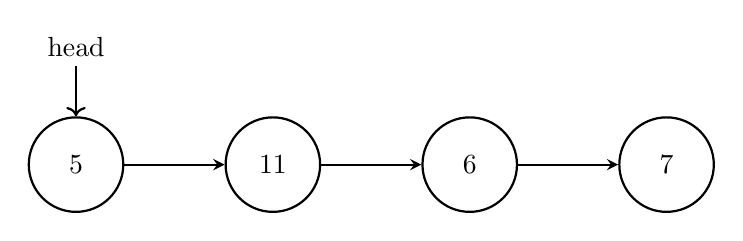
\begin{tikzpicture}[
            node/.style={circle, draw, minimum size=1.2cm, thick},
            arrow/.style={->, >=stealth, thick}
        ]

        % Nodes (circles)
        \node[node] (n1) at (0,0) {5};
        \node[node] (n2) at (2.5,0) {11};
        \node[node] (n3) at (5,0) {6};
        \node[node] (n4) at (7.5,0) {7};

        % Arrows connecting nodes
        \draw[arrow] (n1) -- (n2);
        \draw[arrow] (n2) -- (n3);
        \draw[arrow] (n3) -- (n4);

        % Head label and arrow
        \node[] (head) at (0,1.5) {head};
        \draw[->, black, thick] (head) -- (n1);
      \end{tikzpicture}
      \caption{The following diagram represents a linked list. But in reality, the elements are all located random in memory and can only be found by references. } 
      \label{fig:linked_list}
    \end{figure}
  \end{definition}

  \begin{algo}[Retrieve $i$th Element from Linked List]
    Given a linked list of size $n$ and some $1 \leq i \leq n$, retrieval of the $i$th value is $O(i)$, which 
    \begin{enumerate}
      \item in best case is $O(1)$ if $i$ is a fixed number not dependent on $n$. 
      \item in worst case is $O(n)$ if $i = n$, since we have to traverse through the $n-1$ nodes. 
    \end{enumerate}
  \end{algo}

  This is the first time we actually look at a nontrivial algorithm. 

  \begin{algo}[Insert Element to $i$th Index in Linked List]
    To add value $b$ as the $i$th element of a linked list, we must have first traverse through to the $i-1$ node $a_{i-1}$, then set it to point to $b$, and finally have $b$ point to $a_{i}$. The runtime is dominated by the first step of traversing, which is $O(i)$ and may be 
    \begin{enumerate}
      \item $\Theta(1)$ in the best case when $i=1$, or 
      \item $\Theta(n)$ in the worst case when $i=n$
    \end{enumerate}
    Note that this allows us to easily add to the beginning of a linked list, which was inefficient for regular lists. However, we now sacrifice the easy cost of adding to the end of the list, which worsened from $\Theta(1)$ to $\Theta(n)$. 

    \begin{algorithmic}[1]
      \Procedure{AddElementToLinkedList}{}
      % Variable initialization
      \State Linked list $L$, value $b$, index $i$ to insert to 
      \State $h, c \gets L$ \Comment{create references to head and current} 
      
      \For{$i \gets 1 \ldots i-2$} 
        \State $c \gets c.next$
      \EndFor 

      \State $t \gets c.next$  \Comment{Store temporary reference to $a_{i}$}
      \State $c.next \gets b$  \Comment{$a_{i}$ points to $b$}
      \State $b.next \gets t$  \Comment{$b$ points to $a_{i+1}$} 
      \State \Return{$h$} \Comment{return head}
      \EndProcedure
    \end{algorithmic}
  \end{algo}

  \begin{algo}[Modify $i$th Element in Linked List]
    Modifying is trivial since you just traversing the linked list to the $i$th node and then replace the value there. 
    \begin{enumerate}
      \item If $i$ is constant, then this is $\Theta(1)$. 
      \item If $i = n$ in the worst case, then this is $\Theta(n)$. 
    \end{enumerate}
  \end{algo}

  \begin{algo}[Contains in a Linked List]
    Checking containment just requires us to loop through all nodes and then determine whether our input value is equal to the value stored in the node. This requires us to loop through the entire list so is $\Theta(n)$. 
  \end{algo}

  \begin{algo}[Delete $i$th Element from Linked List]
    Deleting $a_i$ is the same logic as adding. We traverse the linked list until we get to node $a_{i-1}$, and then we set it to point to $a_{i+1}$. The runtime is dominated by the first step of traversing, which is $O(i)$ and may be 
    \begin{enumerate}
      \item $\Theta(1)$ in the best case when $i=1$, or 
      \item $\Theta(n)$ in the worst case when $i=n$
    \end{enumerate}

    \begin{algorithmic}[1]
      \Procedure{DeleteElementFromLinkedList}{}
      % Variable initialization
      \State Linked list $L$, index $i$ to insert to 
      \State $h, c \gets L$ \Comment{create references to head and current} 
      
      \For{$i \gets 1 \ldots i-2$} 
        \State $c \gets c.next$
      \EndFor 

      \State $c.next \gets c.next.next$ \Comment{Skip the next node and have it point to the node after}
      \State \Return{$h$} \Comment{return head}
      \EndProcedure
    \end{algorithmic}
  \end{algo} 

  \begin{algo}[Concatenating 2 Linked Lists]
    Given two linked lists $L_1, L_2$ of size $n, m$,  concatenating them to list $L_1 \oplus L_2$ is $O(n + m)$.
    \begin{algorithmic}[1]
      \Procedure{ConcatenateLinkedLists}{}
      \State Linked lists $L_1, L_2$
      \State $h_1, c_1 \gets L_1$ \Comment{create references to head and current of $L_1$} 
      
      \If{$h_1 = \text{null}$} \Comment{if $L_1$ is empty}
        \State \Return{$L_2$} \Comment{return $L_2$ as the result}
      \EndIf
      
      \While{$c_1.\text{next} \neq \text{null}$} \Comment{traverse to the end of $L_1$}
        \State $c_1 \gets c_1.\text{next}$
      \EndWhile
      
      \State $c_1.\text{next} \gets L_2$ \Comment{link the last node of $L_1$ to the head of $L_2$}
      
      \State \Return{$h_1$} \Comment{return the head of the concatenated list}
      \EndProcedure
    \end{algorithmic}
  \end{algo}

  \begin{algo}[Reversing a Linked List]
    Given a linked list $L$ of size $n$, reversing it has time complexity $O(n)$ as we need to traverse the entire list once. There is both an iterative and recursive approach. 
    
    \begin{algorithmic}[1]
      \Procedure{IterativeReverseLinkedList}{}
      \State Linked list $L$
      \State $prev \gets \text{null}$ \Comment{previous node, initially null}
      \State $curr \gets L$ \Comment{current node, starts at head}
      \State $next \gets \text{null}$ \Comment{to temporarily store the next node}
      
      \While{$curr \neq \text{null}$}
        \State $next \gets curr.\text{next}$ \Comment{store next node}
        \State $curr.\text{next} \gets prev$ \Comment{reverse the pointer}
        \State $prev \gets curr$ \Comment{move prev forward}
        \State $curr \gets next$ \Comment{move curr forward}
      \EndWhile
      
      \State \Return{$prev$} \Comment{prev is the new head of reversed list}
      \EndProcedure
    \end{algorithmic} 
    
    \begin{algorithmic}[1]
      \Procedure{RecursiveReverseLinkedList}{$head$}
      \If{$head = \text{null}$ or $head.\text{next} = \text{null}$}
        \State \Return{$head$} \Comment{Base case: empty list or single node}
      \EndIf
      
      \State $newHead \gets \Call{RecursiveReverseLinkedList}{head.\text{next}}$ \Comment{Reverse the rest}
      \State $head.\text{next}.\text{next} \gets head$ \Comment{Make next node point to current}
      \State $head.\text{next} \gets \text{null}$ \Comment{Remove original next pointer}
      
      \State \Return{$newHead$} \Comment{Return the new head (original tail)}
      \EndProcedure
    \end{algorithmic}
  \end{algo} 

  \begin{definition}[Doubly Linked List]
    A \textbf{doubly linked list} contains a sequence of nodes where each node contains an object for its element, a reference to the next node, and a reference to the previous node.
    \begin{enumerate}
      \item The variable which points to the 1st node is called the \textbf{head}. As with singly linked lists, this variable represents the \textit{entire list} but is just a pointer to the first node.
      \item A sequence of nodes, each containing the element, a reference to the next node, and a reference to the previous node.
      \item The final \textbf{tail} node containing the element, a reference to $\texttt{null}$ for its next pointer, and a reference to the second-to-last node for its previous pointer.
    \end{enumerate}
    Similar to singly linked lists, we will use \textbf{one-indexing} for doubly linked lists, i.e., the head node is located at index $1$.
    \begin{figure}[H]
      \centering 
      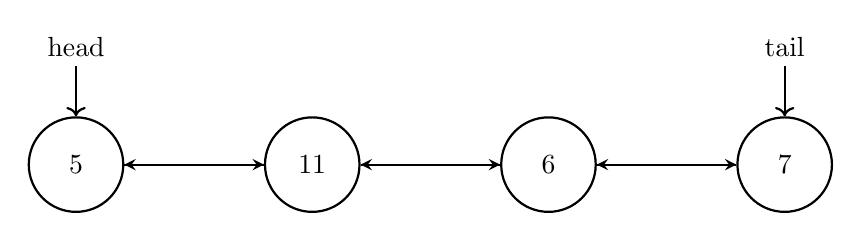
\begin{tikzpicture}[
            node/.style={circle, draw, minimum size=1.2cm, thick},
            arrow/.style={->, >=stealth, thick}
        ]
        % Nodes (circles)
        \node[node] (n1) at (0,0) {5};
        \node[node] (n2) at (3,0) {11};
        \node[node] (n3) at (6,0) {6};
        \node[node] (n4) at (9,0) {7};
        % Forward arrows connecting nodes
        \draw[arrow] (n1) -- (n2);
        \draw[arrow] (n2) -- (n3);
        \draw[arrow] (n3) -- (n4);
        % Backward arrows connecting nodes
        \draw[arrow] (n2) -- (n1);
        \draw[arrow] (n3) -- (n2);
        \draw[arrow] (n4) -- (n3);
        % Head label and arrow
        \node[] (head) at (0,1.5) {head};
        \draw[->, black, thick] (head) -- (n1);
        % Tail label and arrow (optional)
        \node[] (tail) at (9,1.5) {tail};
        \draw[->, black, thick] (tail) -- (n4);
      \end{tikzpicture}
      \caption{This diagram represents a doubly linked list. Forward pointers are shown in black, while backward pointers are shown in red. As with singly linked lists, the elements are located randomly in memory and can only be found through references. The presence of backward pointers allows for bidirectional traversal.}
      \label{fig:doubly_linked_list}
    \end{figure}
  \end{definition} 

  While we have to keep an extra pointer for every node in memory, this allows for simpler and sometimes more efficient implementations of the algorithms. For example, reversing a linked list can be done by simply swapping the previous and next pointers in each node. We can also add to and remove from both the front and back of a linked list in $O(1)$ time. 

  \begin{definition}[Circular Linked List]
    A \textbf{circular linked list} is a variation of a linked list where the last node, instead of pointing to null, contains a reference back to the first node, forming a circle or loop. This structure can be applied to both singly and doubly linked lists:
    \begin{enumerate}
      \item In a circular singly linked list, the last node's next pointer references the head node.
      \item In a circular doubly linked list, the last node's next pointer references the head node, and the head node's previous pointer references the last node.
    \end{enumerate}
    This circular nature allows traversal of the entire list starting from any node, as following the next pointers will eventually cycle through all nodes.
    \begin{figure}[H]
      \centering 
      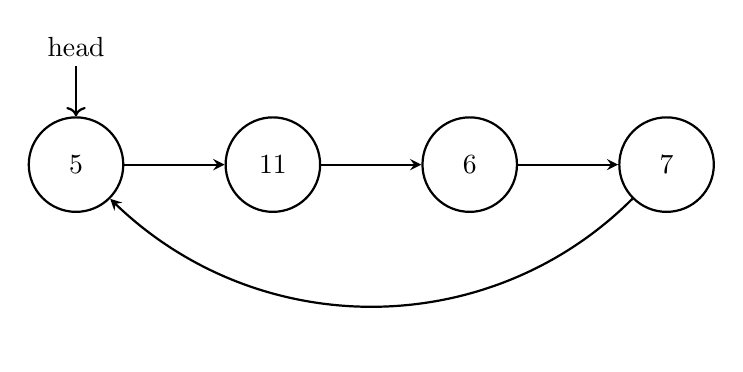
\begin{tikzpicture}[
            node/.style={circle, draw, minimum size=1.2cm, thick},
            arrow/.style={->, >=stealth, thick}
        ]
        % Nodes (circles)
        \node[node] (n1) at (0,0) {5};
        \node[node] (n2) at (2.5,0) {11};
        \node[node] (n3) at (5,0) {6};
        \node[node] (n4) at (7.5,0) {7};
        % Arrows connecting nodes (straight)
        \draw[arrow] (n1) -- (n2);
        \draw[arrow] (n2) -- (n3);
        \draw[arrow] (n3) -- (n4);
        % Circular connection
        \draw[arrow, bend left=45] (n4) to (n1);
        % Head label and arrow
        \node[] (head) at (0,1.5) {head};
        \draw[->, thick] (head) -- (n1);
      \end{tikzpicture}
      \caption{A circular singly linked list where the last node points back to the head node, creating a cycle. This structure eliminates the concept of a ``null end'' found in standard linked lists.}
      \label{fig:circular_linked_list}
    \end{figure}
  \end{definition}

  Let's introduce one more data structure. Note that even though our basic linked list solves the problem of adding in the beginning, in order to add in the middle or end, we must get to that position (which is $O(n)$ time) before we are able to utilize our $O(1)$ add. This is quite inefficient, especially when we do repeated adding, so we should keep track of certain "markers" that indicate where our current node is. \textit{Iterators} do this naturally, so we would like to implement some current notion of position. 

  \begin{definition}[Iterator]
    An \textbf{iterator} is a structure that maintains a reference a \textit{current position} within a list, along with methods to move the iterator to the next node (and previous node in doubly linked lists). 

    \begin{figure}[H]
      \centering 
      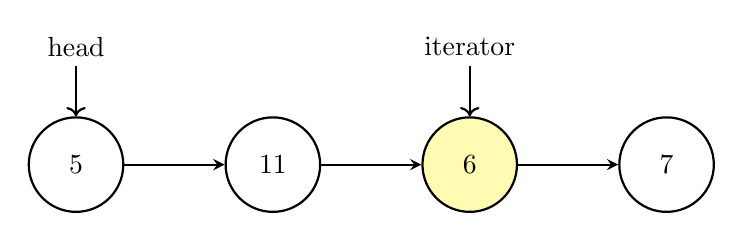
\begin{tikzpicture}[
            node/.style={circle, draw, minimum size=1.2cm, thick},
            arrow/.style={->, >=stealth, thick}
        ]
        % Nodes (circles)
        \node[node] (n1) at (0,0) {5};
        \node[node] (n2) at (2.5,0) {11};
        \node[node, fill=yellow!30] (n3) at (5,0) {6};
        \node[node] (n4) at (7.5,0) {7};
        % Arrows connecting nodes
        \draw[arrow] (n1) -- (n2);
        \draw[arrow] (n2) -- (n3);
        \draw[arrow] (n3) -- (n4);
        % Head label and arrow
        \node[] (head) at (0,1.5) {head};
        \draw[->, thick] (head) -- (n1);
        % Iterator label and arrow
        \node[] (iter) at (5,1.5) {iterator};
        \draw[->, thick] (iter) -- (n3);
      \end{tikzpicture}
      \caption{A linked list with an iterator currently positioned at the node containing the value 6. The iterator allows for immediate access to this position without traversing from the head.}
      \label{fig:linked_list_iterator}
    \end{figure}
  \end{definition}

  At first glance it may seem like iterators are just lists with less functionality, but we will see later that even non-array-like data structures can be turned into lists.  

\subsection{Stacks} 

  A stack is pretty much a list with a more limited set of operations, so whatever we can do with a stack we can do with a list. However, it is worth mentioning as its own data structure since it allows us to work with a simpler interface. 

  \begin{definition}[Stack]
    \label{def:stack}
    A \textbf{stack} is a data structure that stores data in the \textit{last-in-first-out (LIFO)} paradigm, which means that we can push (insert) elements into a stack $S$ and pop (remove) the last element that was pushed. 

    \begin{figure}[H]
      \centering 
      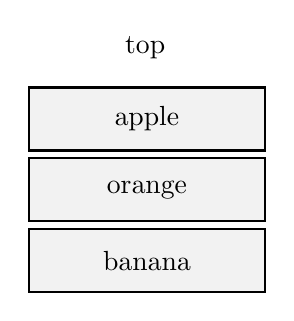
\begin{tikzpicture}[
        box/.style={rectangle, draw, thick, minimum width=3cm, minimum height=0.8cm, fill=gray!10}
        ]
        % Stack base
        \draw[thick] (0,0) -- (3,0);
        
        % Stacked items
        \node[box] (banana) at (1.5,0.4) {banana};
        \node[box] (orange) at (1.5,1.3) {orange};
        \node[box] (apple) at (1.5,2.2) {apple};
        
        \node[right] at (1.1,3.1) {top};
      \end{tikzpicture}
      \caption{We can literally imagine the elements of this list as ``stack.'' If you want to remove something from the stack, of course you have to remove the top element. } 
      \label{fig:stack}
    \end{figure}
  \end{definition} 

  The actual implementation can be done in many ways, either through a list or a linked list. 

  \begin{algo}[Push onto Stack]
    To push, i.e. add an element, onto the stack, we can 
    \begin{enumerate}
      \item insert to the end of a list, which is amortized $\Theta(1)$. 
      \item insert to the head of a singly linked list, which is $\Theta(1)$. 
    \end{enumerate}
  \end{algo}

  \begin{algo}[Pop from Stack]
    To pop, i.e. remove the last element pushed, from the (top of the) stack, we can 
    \begin{enumerate}
      \item remove the last element of a list, which is $\Theta(1)$. 
      \item move the head pointer to the second node and return the first node, which is $\Theta(1)$. 
    \end{enumerate}
  \end{algo}

  \begin{algo}[Peek into Stack]
    To peek, i.e. retrieve only the value at the top of the stack, we can 
    \begin{enumerate}
      \item return the last element of a list, which is $\Theta(1)$. 
      \item return the value of the head of the linked list, which is $\Theta(1)$. 
    \end{enumerate}
  \end{algo}

\subsection{Queues}

  \begin{definition}[Queue]
    A \textbf{queue} is an data structure that stores elements in the \textit{first-in-first-out (FIFO)} paradigm, which means that we can enqueue (insert) elements into a queue $Q$ and \textit{dequeue} (remove) elements in the order that they were pushed. 

    \begin{figure}[H]
      \centering 
      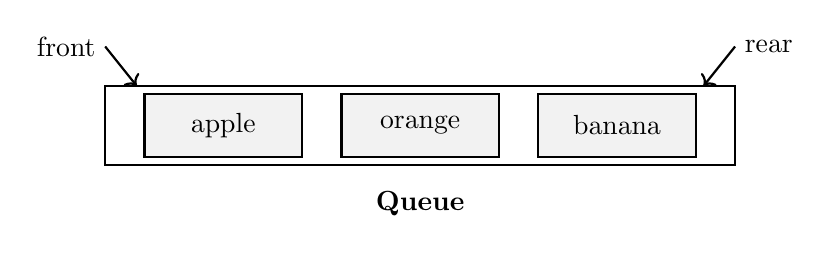
\begin{tikzpicture}[
        box/.style={rectangle, draw, thick, minimum width=2cm, minimum height=0.8cm, fill=gray!10}
        ]
        % Queue container
        \draw[thick] (0,0) rectangle (8,1);
        
        % Queue items
        \node[box] (apple) at (1.5,0.5) {apple};
        \node[box] (orange) at (4,0.5) {orange};
        \node[box] (banana) at (6.5,0.5) {banana};
        
        % Queue label
        \node[font=\bfseries] at (4,-0.5) {Queue};
        
        % Front and rear pointers
        \draw[->, thick] (0,1.5) -- (0.4,1);
        \node[left] at (0,1.5) {front};
        
        \draw[->, thick] (8,1.5) -- (7.6,1);
        \node[right] at (8,1.5) {rear};
      \end{tikzpicture}
      \caption{This is just like how a queue works. Whatever has been waiting in the queue the longest is the one that is removed first (at the front).} 
      \label{fig:queue}
    \end{figure}
  \end{definition} 

  Unlike a stack, which can be implemented with a list or linked list, for queues we must implement with a linked list with both a head and a tail pointer (or a doubly linked list). If we use a list, then to enqueue in $\Theta(1)$ time we must have it add to the end of the list, but when dequeuing, we must remove from the front of a list, which is inevitably $\Theta(n)$. The linked list has the opposite problem. Dequeuing is easy since we can shift the head node, but enqueuing requires us to traverse to the end before adding another node, which is $\Theta(n)$. In fact, Python implements this as a double ended queue.\footnote{\texttt{from collections import deque} where deque stands for double ended queue.} However, we will work with the minimal data structure of a singly linked list with a head and tail pointer. 

  \begin{algo}[Enqueue onto Queue]
    To enqueue an element $b$, we can have the tail pointer $a_n$ point to $b$ and update the tail pointer to $b$. This is $\Theta(1)$. 
  \end{algo}

  \begin{algo}[Dequeue onto Queue]
    To dequeue, we can return the head $a_1$ and update the head pointer to $a_2$.  
  \end{algo}

  \begin{algo}[Peek into Queue]
    To peek into the queue, we can simply return the value of the head pointer $a_1$. 
  \end{algo}


\section{Hash-Based Data Structures} 

\subsection{Hashing}

  One of the most important applications of hashing and probabilistic algorithms is in cryptography. For example, when you generate a RSA keypair, you must choose two 128-bit prime numbers which serve as your private key. State of the art methods simply generate a random 128-bit prime number perform \textit{independent} randomized probabilistic tests with error rate $\epsilon$. Given that this is independent, simply running this tests $k$ times reduces our error exponentially to $\epsilon^k$, practically guaranteeing primality. In Bitcoin and Ethereum wallets, hardened child key derivation functions in hierarchical determinstic wallets hash subsets of the parent key to generate both the child keys and their seeds.\footnote{For an implementation of both, look at my blockchain implementation \href{https://github.com/mbahng/blade/blob/main/backend/src/crypt/primes.js\#L61}{here}} 

  Assume we want to map keys from some \textbf{universe} $U$ into a smaller set $[N] = \{1, \ldots, N\}$ of $N$ bins. The algorithm will have to handle some dataset $S \subset U$ of $|S| = M$ keys.\footnote{For example, think of all possible strings as $U$ and all $256$-bit numbers as $N = 2^{256}$. $S$ in this case $S$ may be the set of all addresses on a blockchain. This is SHA256, and to date there is no known hash collisions, though there are a few for SHA1.} We want to store $S$ with efficient performance in 
  \begin{enumerate}
    \item \texttt{Find(x)}, which returns true if $x \in S$
    \item \texttt{Insert(x)} 
    \item \texttt{Delete(x)}
    \end{enumerate}
  This is essentially a set. If one is new to hashing, we could try to use a balanced binary search tree or a heap (implemented as a red-black tree or some other variant), which can do all three operations in $O(\log(N))$ time. If we had access to a randomized function $h: U \rightarrow [N]$, with the property that for a fixed $x \in U$, $h(x) \sim \mathrm{Multinomial}(N)$, then by linearity of expectation\footnote{Note that this is not $\mathbb{P}_{x, y}$ since $x, y$ are not random variables. They are fixed, and $h(x), h(y)$ are the random variables. }
  \begin{equation}
    \mathbb{P}(h(x) = h(y)) = \mathbb{E}[\mathbbm{1}_{h(x) = h(y)}] = \frac{N}{N^2} = \frac{1}{N}
  \end{equation}
  This is great, but this is also random, which means that we are not guaranteed to map to the same bin across time. If we add time-invariance, this is pretty much a hash function, which is really deterministic, but we like to call it psuedo-random. 

  So what if there are collisions? They are inevitable anyways even with a completely random function, but minimizing them will give us the best runtime performance. There are a two main ways to approach this. 
  \begin{enumerate}
    \item At each bin, store the head of a linked list, BST, or another hash table. You would incur an additional linear, logarithmic, or constant cost of traversing this data structure for each operation.  
    \item Look for another bin. We can just look at $h(x) + 1$ or $h(h(x))$ (or really any deterministic function $f(h(x))$) if $h(x)$ is occupied. 
  \end{enumerate}

  This is what we have to work with here, so we would like to modify our assumptions. Therefore, we can achieve good performance by reducing the collisions and by improving how we deal with collisions. We will focus on the first part, and we would like for our hash functions to have some nice properties, which we will define. The most intuitive way is to treat $x, y$ as random variables uniformly sampled from $U$, and then we would like $\mathbb{P}(h(x) = H(y)) \approx 1/N$. However in practice, this is not the case since our subdomain $S$ is already fixed, yet may be unknown. Therefore given any function $h$, we can construct an adversarial sequences of inputs that will all map to the same bin. We must therefore consider a \textit{family} of hash functions. 

  \begin{definition}[Universal Hashing]
    A family of hash functions $H = \{h : U \rightarrow [N] \}$ is \textbf{universal} if for any fixed $x, y \in U$, 
    \begin{equation}
      \mathbb{P}_{h} \big( h(x) = h(y) \big) \leq \frac{1}{N}
    \end{equation}
    where $h$ is drawn uniformly. If the bound is $2/N$ then it is called \textbf{near-universal}, and what's important is the $N$ in the denominator. This polynomial decay in collision probabilities is exactly what we need for constant operation time. That is, given query $x$, let the random variable $X$ be the number of operations we must do to find $X$, which consists of $1$ pointer traversal plus some other amount of traversals (e.g. through a linked list) if collision, say which is $C_n$. So we have 
    \begin{equation}
      X = 1 + \sum_{y \in S} Q_y
    \end{equation}
    where $1$ comes from the initial pointer traversal in hashing, and Bernoulli $Q_y = 1$ if $h(y) = h(x)$.\footnote{This may not be $1$ since we may have to do more than 1 additional traversal, e.g. in linked lists. But we assume the extra cost is bounded by a constant.} Then, by linearity of expectation combined with the bound on probability of collision we have 
    \begin{equation}
      \mathbb{E}[X] = 1 + \sum_{y \in S} \mathbb{E}[Q_y] = 1 + |S| \cdot \mathbb{P}(h(x) = h(y)) = 1 + \frac{|S|}{N}
    \end{equation} 
    which is constant. 
  \end{definition} 

  If $H$ is the set of all functions from $U$ to $[N]$, then this universal property is trivially satisfied since 
  \begin{equation}
      \mathbb{P}_{h} \big( h(x) = h(y) \big) = \frac{1}{N}
  \end{equation}
  But this is quite a complex function class and $h$ may not be easy to store, i.e. may not be analytic. The question now becomes whether we can achieve universality with a smaller class. It turns out yes, and the obvious use is to use cyclic groups. 

  \begin{lemma}[Carter-Wegman 71]
    Suppose $U = \{0, 1, \ldots, M-1\}$. We choose a prime $p \geq M$\footnote{It is guaranteed that a prime exists between $m$ and $2m$.} and construct the family 
    \begin{equation}
      H = \{h_a (x) = (ax \mathrm{ mod } p ) \mathrm{ mod } N \mid a = 0, \ldots, p-1 \}
    \end{equation}
    We claim this is near-universal. 
  \end{lemma}
  \begin{proof}
    We treat $x$ as the generator of this group, and then $ax \mathrm{ mod } p = a^\prime x { mod } p$ iff $a = a^\prime$. Therefore, 
    \begin{equation}
      \mathbb{P}_a (h_a (x) = h_a (y)) = \mathbb{P}_a \big( (ax - ay) \mathrm{ mod } p = N k \big)
    \end{equation}
    for some $k$. If $a = 0$, then everything collides, but if $a \neq 0$ and $x \neq y$, then $ax - ay$ must have a difference of exactly a multiply of $N$, which happens with probability $1/N$. Therefore, we have 
    \begin{equation}
      \mathbb{P}_a (h_a (x) = h_a (y)) = \mathbb{P}(a = 0) + \mathbb{P}(a \neq 0) \cdot \frac{1}{N} = \frac{1}{p} + \frac{p-1}{p} \cdot \frac{1}{N} < \frac{2}{N} 
    \end{equation}
    since $p > N$. 
  \end{proof}

  Therefore, to hash, 
  \begin{enumerate}
    \item we choose a prime $p \geq m = |U|$. 
    \item choose $a \in \{0, 1, \ldots, p-1\}$ at random. 
    \item Use $h_a(x) = (ax \mathrm{ mod } p ) \mathrm{ mod } N$ to hash everything.\footnote{We do not change $a$ every time we hash. }
  \end{enumerate}

  \begin{example}
    Let $n$ be a fixed prime number and 
    \begin{equation}
      H = \{h_{a, b} (x, y) = ax + by \mathrm{ mod } n : a, b \in [n] \}
    \end{equation} 
    We claim that this is universal. Let $x = (x_1, x_2)$ and $y = (y_1, y_2)$ be arbitrary pairs of integers where $x \neq y$. WLOG, assume $x_2 \neq y_2$. Then 
    \begin{equation}
      \mathbb{P}(h_{a, b} (x) = h_{a, b} (y)) = \mathbb{P}(a x_1 + b x_2 = a y_1 + b y_2) = \mathbb{P}\big( a (x_1 - y_1) = b (y_2 - x_2) \big)
    \end{equation} 
    Suppose that we pick $a$ first and we compute the conditional probability. Then the LHS is a constant, and for this to hold in a cyclic group, $b$ must equal $c (y_2 - x_2)^{-1}$, which occurs with probability $1/N$. Using LOTP the joint probability is also $1/N$. 
  \end{example}

\subsection{Set} 

  Sets are conceptually the same as mathematical sets. 

  \begin{definition}[Set]
    A \textbf{set} is an unordered data structure that stores unique elements. 
    \begin{enumerate}
      \item Add is $O(1)$. 
      \item Remove is $O(1)$. 
      \item Retrieval and contains is $O(1)$. 
    \end{enumerate}
  \end{definition}

\subsection{Map} 

  A hash table is an array of key value pairs. But rather than adding to positions in order from 0, 1, 2, ..., we will calculate the hash of the key, which would return an int that specifies where we store this key-value pair. So to store, $\texttt{<"ok", 8>}$, we will calculate $\texttt{hash("ok") == 5}$ and store it in the 5th index.
  \begin{lstlisting}
    0 
    1 
    2 <"hi", 5>
    3 
    4 
    5 <"ok", 8>
    6 
    7 
  \end{lstlisting}
  We can immediately see how this makes search easier, since if we want to find the value associated with the key "ok", then we can calculate the hash of it to find the index and look it up on the array. 

  \begin{definition}[Maps]
    A \textbf{map}, also called a \textbf{hash table}, is an unordered data data structure that stores key-value pairs.   
    \begin{enumerate}
      \item Add is $O(1)$. 
      \item Remove is $O(1)$. 
      \item Retrieval and contains is $O(1)$. 
    \end{enumerate}
  \end{definition}

  So running $\texttt{get(key)}$ on a HashMap looks up position $\texttt{hash(key)}$ in the hash table and returns the value there. Immediately, we see that if $\texttt{hash}$ is not injective (which it isn't), then we can run into collisions. This is solved using chaining or bucketing. Bucketing basically takes each index in the array and stores not just one key-value pair, but a list of key-value pairs. So basically, when we want to search for the value of a key, we compute the index of it with $\texttt{hash(key)}$, which would return a list of key-value pairs. 

  Obviously, if we create a custom $\texttt{hashCode()}$ method that trivially maps to 0, then we would just have one giant list in the bucket at index 0, which is no more efficient than a list search. So, we should ideally assume that given N pairs with M buckets, our hashing function is built so that the probability of two random (unequal keys) hash to the same bucket is 1/M. Note that this hash function is completely deterministic. We should talk about runtime/memory tradeoff. Given N pairs and M buckets (with SUHA): 
  \begin{enumerate}
      \item $N >> M$ means too many pairs in too few buckets, so runtime inefficient 
      \item $M >> N$ means too many buckets for too few pairs, so memory wasteful 
      \item $M$ slightly larger than $N$ is the sweet spot.
  \end{enumerate}
  To maintain an ideal ratio, we basically create a new larger table (with geometric resizing) and rehash/copy everything until we reach it.



\section{Graph-Based Data Structures} 

  So far, arrays and hashing are the two most intuitive ways that we would store data. The next set of data structures not only store values, but it store the \textit{interactions} between these values. While it may not seem as natural to the new-comer, trees---and more generally, graphs---are a natural way to store real-world data. 

  At this point, you should be familiar with the concept of \textit{recursive algorithms}, which naturally appears in graphs (e.g. a subtree of a tree is a tree itself). Unlike the previous data structures, the elementary operations on graphs (e.g. insert, remove, etc.) are not as trivial, and so the conceptual difficulty significantly jumps from here.  

\subsection{Graphs}

  \begin{definition}[Undirected Graphs]
    An \textbf{undirected graph} $G(V, E)$ is a tuple, where $V = \{v_1, \ldots, v_n\}$ is the vertex set and $E = \{\{v_i, v_j\}\}$ is the edge set. 
    \begin{enumerate}
      \item The \textbf{degree} $d_v$ of a vertex $v$ is the number of edges incident to it. 
      \item A \textbf{path} is a sequence of vertices where adjacent vertices are connected by a path in $E$. It's \textbf{length} is the number of edges in the path. 
      \item A \textbf{cycle/circuit} is a path that has the same start and end. 
      \item A graph is \textbf{connected} if for every pair of vertices $e_i, e_j \in E$, there is a path from $e_i$ to $e_j$. 
      \item A \textbf{connected component} is a maximal subset of connected vertices. 
    \end{enumerate}
    The \textbf{size} of a graph is a tuple $(n, m) = (|V|, |E|)$. 
  \end{definition}

  \begin{definition}[Directed Graph]
    A \textbf{directed graph} $G(V, E)$ is a tuple, where $V = \{v_1, \ldots, v_n\}$ is the vertex set and $E = \{(v_i, v_j)\}$ is the edge set (note that it is a set of tuples, so $(i, j) \neq ( j, i)$).
    \begin{enumerate}
      \item The \textbf{in/out degree} $d_{v, i}, d_{v, o}$ of a vertex $v$ is the number of edges going in to or out from $v$. 
      \item A \textbf{path} is a sequence of vertices where adjacent vertices are connected by a path in $E$. It's \textbf{length} is the number of edges in the path. 
      \item A \textbf{cycle/circuit} is a path that has the same start and end. 
      \item A directed graph is \textbf{strongly connected} if for every pair of vertices $e_i, e_j \in E$, there is a path from $e_i$ to $e_j$.\footnote{Obviously, a connected undirected graph is also strongly connected.}
      \item A \textbf{strongly connected component} is a maximal subset of connected vertices. 
    \end{enumerate}
  \end{definition}

  In fact, from these definitions alone, we can solve an ancient puzzle called \textit{the Bridges of Konigsberg}. Euler, in trying to solve this problem, had invented graph theory. 

  \begin{example}[Bridges of Konigsberg]
    Is there a way to walk that crosses each bridge \textit{exactly} once? 

    \begin{figure}[H]
      \centering
      \begin{subfigure}[b]{0.48\textwidth}
      \centering
        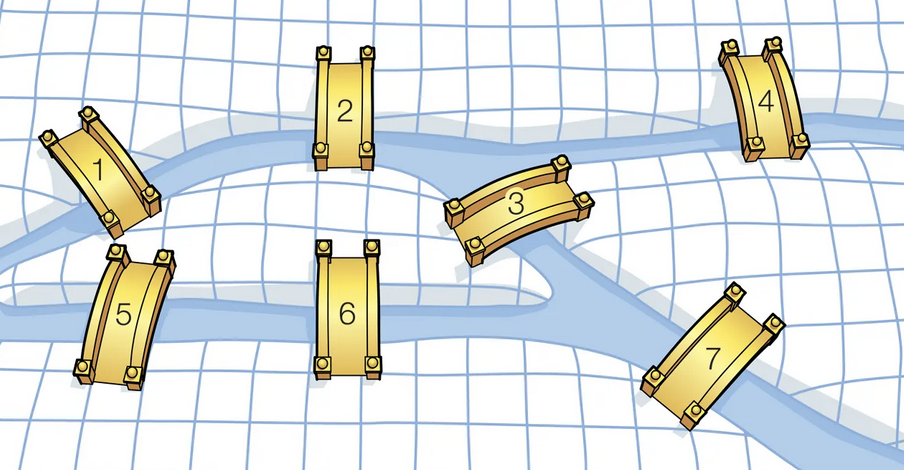
\includegraphics[scale=0.4]{img/bridges.png}
        \caption{Figure of the bridges of Konigsberg.}
        \label{fig:bridges}
      \end{subfigure}
      \hfill 
      \begin{subfigure}[b]{0.48\textwidth}
      \centering
        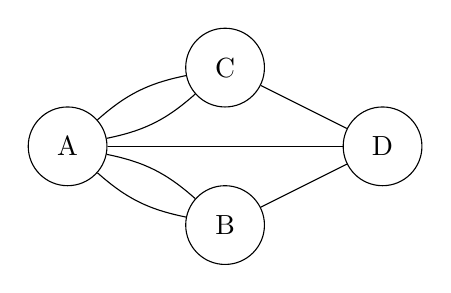
\begin{tikzpicture} 
          \tikzstyle{every node}=[circle, draw, minimum size=1cm]
          
          \node (A) at (0,0) {A};
          \node (B) at (2,-1) {B};
          \node (C) at (2,1) {C};
          \node (D) at (4,0) {D}; 
                
          \draw (A) to[bend left=15] (B);
          \draw (A) to[bend right=15] (B);
          \draw (A) to[bend left=15] (C);
          \draw (A) to[bend right=15] (C);
          \draw (A) -- (D);
          \draw (B) -- (D);
          \draw (C) -- (D);
        \end{tikzpicture}
        \caption{Graph representation. }
        \label{fig:graph_bridges}
      \end{subfigure}
      \caption{It can be decomposed into this undirected graph.}
      \label{fig:konigsberg}
    \end{figure}
     
    Euler's observation is that except for start and end points, a talk leaves any vertex by different edge that the incoming edge. Therefore, the degree (number of edges incident on it) must have an even number, so all but 2 vertices must have an even degree. Since every vertex has an odd degree, there is no way of doing it. 
  \end{example}

  In addition to the \textit{adjacency list} representation, another way in which we represent a directed graph is through \textit{adjacency matrices}. 

  \begin{definition}[Adjacency Matrix]
    In a finite directed graph $(V, E)$, we can construct a bijection from $V$ to the natural numbers and so we label each element in $V$ with $i \in \mathbb{N}$. Then, we can construct a matrix $A$ such that 
    \begin{equation}
      A_{ij} = \begin{cases} 1 & \text{ if } (i, j) \in E \\ 0 & \text{ if } (i, j) \not\in E \end{cases}
    \end{equation}
  \end{definition}

  \begin{example}[Adjacency List vs Matrix]
    Given a graph, we can completely represent it with a list of adjacent vertices for each vertex or an adjacency matrix. 
    \begin{center}
    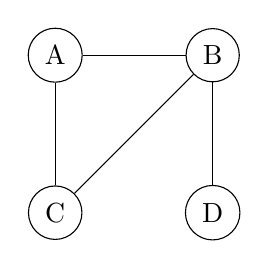
\begin{tikzpicture}
      \node[circle, draw] (C) at (0,0) {C};
      \node[circle, draw] (D) at (2,0) {D};
      \node[circle, draw] (B) at (2,2) {B};
      \node[circle, draw] (A) at (0,2) {A};

      \draw (A) -- (B);
      \draw (B) -- (C);
      \draw (A) -- (C);
      \draw (B) -- (D);
    \end{tikzpicture}
    \end{center}
    An adjacency list would look something like this 
    \[
    \begin{aligned}
    A &: B, C \\
    B &: A, C, D \\
    C &: A, B \\
    D &: B
    \end{aligned}
    \]
    and the adjacency matrix looks like this: 
    \begin{center}
    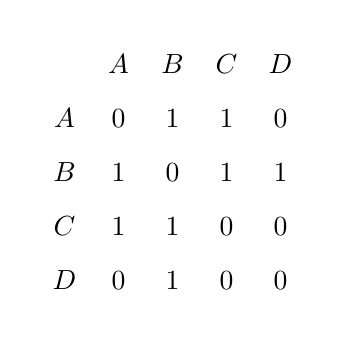
\begin{tikzpicture}
      \matrix[matrix of math nodes, nodes in empty cells,          column sep=-\pgflinewidth, row sep=-\pgflinewidth,          nodes={minimum size=7mm, anchor=center, outer sep=0pt}] (adjacency) {
        & |(a)| A & |(b)| B & |(c)| C & |(d)| D \\
        |(A)| A & 0 & 1 & 1 & 0 \\
        |(B)| B & 1 & 0 & 1 & 1 \\
        |(C)| C & 1 & 1 & 0 & 0 \\
        |(D)| D & 0 & 1 & 0 & 0 \\
      };
    \end{tikzpicture}
    \end{center}
  \end{example}

  While the adjacency matrix does have its advantages and has a cleaner form, usually in sparse graphs this is memory inefficient due to there being an overwhelming number of $0$s. 

  \begin{algo}[Insert Node/Edge in Graph]
    
  \end{algo}

  \begin{algo}[Remove Node/Edge in Graph]
    
  \end{algo}

  \begin{algo}[Contains in Graph]
    
  \end{algo} 

\subsection{Graph Traversal with DFS/BFS}

  Given two $v, s \in V$ either directed or undirected, how can we find a path from $v$ to $s$? We can do with either with DFS or BFS. 

  Now, in order to traverse this graph, we basically want to make an algorithm that starts at a node, prints it value, and then goes to all of its neighbors (which we can access through the adjacency list) to print them out. Thus, this is by nature recursive. We don't want the algorithm to loop around printing nodes infinitely often, so we must create a base case that tells the algorithm to not print out a node. It makes sense to create a set of visited nodes, which we can add to whenever we reach a new node. So, if we ever come onto a node that we have visited, we can just tell the function to do nothing. 

  \begin{algo}[Recursive Depth-First Search]
    The recursive implementation of Depth-First Search explores a graph by recursively visiting each unvisited neighbor, going as deep as possible along each branch before backtracking.
    \begin{algorithm}[H]
      \label{alg:dfs_recursive}
      \begin{algorithmic}[1]
        \Require{Graph $G(V, E)$, start vertex $s$}
        
        \Function{DFS-Recursive}{$G, s$}
          \State visited $\gets \emptyset$ \Comment{Initialize empty set of visited vertices}
          \State \Call{DFS-Visit}{$G, s$, visited}
        \EndFunction
        
        \Function{DFS-Visit}{$G, u$, visited}
          \State Add $u$ to visited
          \State \textit{/* Process vertex $u$ here */}
          \For{each neighbor $v$ of $u$ in $G$}
            \If{$v \notin$ visited}
              \State \Call{DFS-Visit}{$G, v$, visited}
            \EndIf
          \EndFor
        \EndFunction
      \end{algorithmic}
    \end{algorithm}
  \end{algo}

  Though recursion really makes this simple, we can construct an iterative approach that uses stacks. Note that in recursion, we are really making a call stack of different functions. We can be explicit about this by actually implementing a stack, which would store all the nodes that we have discovered, but not yet explored from )i.e. all the current nodes). At each iteration, we would pick a node to continue exploring, and since this is a DFS, we would want to implement a LIFO stack so that the last element we input in is the first thing that we should explore from, i.e. we always explore from the last node discovered. 

  \begin{algo}[Iterative Depth-First Search]
    The iterative implementation of Depth-First Search uses a stack to mimic the function call stack of the recursive implementation. It explores vertices in the same order as the recursive version.
    \begin{algorithm}[H]
      \label{alg:dfs_iterative}
      \begin{algorithmic}[1]
        \Require{Graph $G(V, E)$, start vertex $s$}
        
        \Function{DFS-Iterative}{$G, s$}
          \State visited $\gets \emptyset$ \Comment{Initialize empty set of visited vertices}
          \State stack $\gets$ empty stack
          \State Push $s$ onto stack
          \State Add $s$ to visited
          
          \While{stack is not empty}
            \State $u \gets$ Pop from stack
            \State \textit{/* Process vertex $u$ here */}
            
            \For{each neighbor $v$ of $u$ in $G$}
              \If{$v \notin$ visited}
                \State Add $v$ to visited
                \State Push $v$ onto stack
              \EndIf
            \EndFor
          \EndWhile
        \EndFunction
      \end{algorithmic}
    \end{algorithm}
  \end{algo}

  \begin{example}[DFS Walkthrough]
    Let's conduct DFS on the following graph. 

    \begin{figure}[H]
      \centering
      \begin{subfigure}[b]{0.48\textwidth}
        \centering
        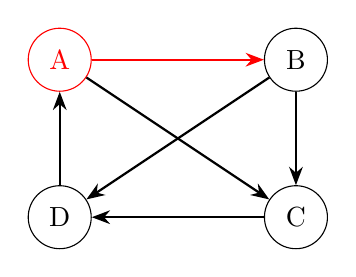
\begin{tikzpicture}[
            node/.style={circle, draw, minimum size=0.8cm},
            arrow/.style={-Stealth, thick}
          ]
          % Define the nodes
          \node[node, red] (A) at (0,0) {A};
          \node[node] (B) at (3,0) {B};
          \node[node] (C) at (3,-2) {C};
          \node[node] (D) at (0,-2) {D};

          % Connect the nodes with directed edges
          \draw[arrow, red] (A) -- (B);
          \draw[arrow] (B) -- (C);
          \draw[arrow] (C) -- (D);
          \draw[arrow] (D) -- (A);
          \draw[arrow] (A) -- (C);
          \draw[arrow] (B) -- (D);
        \end{tikzpicture}
        \caption{You start at $A$ and you add it to your visited set $V = \{A\}$. You look at your neighbors and find that you can explore $B$ or $C$. Let's randomly choose to explore $B$ but keep in mind that you haven't finished exploring from $B$ since there's $C$ left. }
      \end{subfigure}
      \hfill 
      \begin{subfigure}[b]{0.48\textwidth}
        \centering
        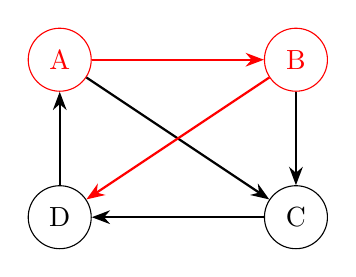
\begin{tikzpicture}[
            node/.style={circle, draw, minimum size=0.8cm},
            arrow/.style={-Stealth, thick}
          ]
          % Define the nodes
          \node[node, red] (A) at (0,0) {A};
          \node[node, red] (B) at (3,0) {B};
          \node[node] (C) at (3,-2) {C};
          \node[node] (D) at (0,-2) {D};

          % Connect the nodes with directed edges
          \draw[arrow, red] (A) -- (B);
          \draw[arrow] (B) -- (C);
          \draw[arrow] (C) -- (D);
          \draw[arrow] (D) -- (A);
          \draw[arrow] (A) -- (C);
          \draw[arrow, red] (B) -- (D);
        \end{tikzpicture}
        \caption{You add $B$ to visited $V = \{A, B\}$ and look at your neighbors $C$ and $D$. Let's just choose $D$ randomly but keep in mind that you have $C$ to explore later, so you haven't finished exploring from $B$ either. Therefore both $A$ and $B$ are both still on your exploration stack.}
      \end{subfigure}

      \begin{subfigure}[b]{0.48\textwidth}
        \centering
        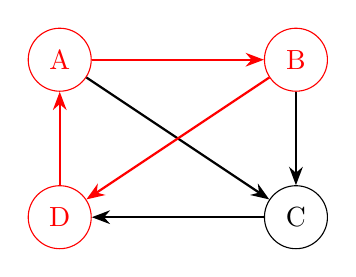
\begin{tikzpicture}[
            node/.style={circle, draw, minimum size=0.8cm},
            arrow/.style={-Stealth, thick}
          ]
          % Define the nodes
          \node[node, red] (A) at (0,0) {A};
          \node[node, red] (B) at (3,0) {B};
          \node[node] (C) at (3,-2) {C};
          \node[node, red] (D) at (0,-2) {D};

          % Connect the nodes with directed edges
          \draw[arrow, red] (A) -- (B);
          \draw[arrow] (B) -- (C);
          \draw[arrow] (C) -- (D);
          \draw[arrow, red] (D) -- (A);
          \draw[arrow] (A) -- (C);
          \draw[arrow, red] (B) -- (D);
        \end{tikzpicture}
        \caption{You add $D$ to visited $V = \{A, B, D\}$. You look at your neighbors and see that you can explore $A$. However it is already in your visited set. Since there are no more neighbors to explore to, you are done exploring from $D$ and don't need to look at it anymore. }
      \end{subfigure}
      \hfill 
      \begin{subfigure}[b]{0.48\textwidth}
        \centering
        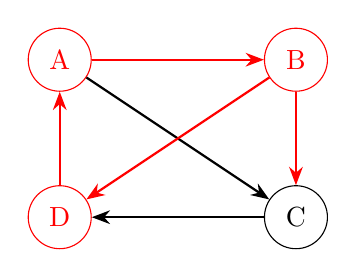
\begin{tikzpicture}[
            node/.style={circle, draw, minimum size=0.8cm},
            arrow/.style={-Stealth, thick}
          ]
          % Define the nodes
          \node[node, red] (A) at (0,0) {A};
          \node[node, red] (B) at (3,0) {B};
          \node[node] (C) at (3,-2) {C};
          \node[node, red] (D) at (0,-2) {D};

          % Connect the nodes with directed edges
          \draw[arrow, red] (A) -- (B);
          \draw[arrow, red] (B) -- (C);
          \draw[arrow] (C) -- (D);
          \draw[arrow, red] (D) -- (A);
          \draw[arrow] (A) -- (C);
          \draw[arrow, red] (B) -- (D);
        \end{tikzpicture}
        \caption{Therefore you look back to where you came from: $B$, and continue exploring from $B$. You go back to $B$ and look at the other nodes you must explore. You've already done $D$ and the only remaining is $C$, which isn't in your visited. }
      \end{subfigure}

      \begin{subfigure}[b]{0.48\textwidth}
        \centering
        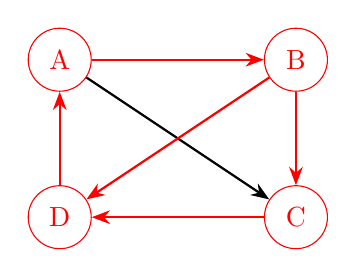
\begin{tikzpicture}[
            node/.style={circle, draw, minimum size=0.8cm},
            arrow/.style={-Stealth, thick}
          ]
          % Define the nodes
          \node[node, red] (A) at (0,0) {A};
          \node[node, red] (B) at (3,0) {B};
          \node[node, red] (C) at (3,-2) {C};
          \node[node, red] (D) at (0,-2) {D};

          % Connect the nodes with directed edges
          \draw[arrow, red] (A) -- (B);
          \draw[arrow, red] (B) -- (C);
          \draw[arrow, red] (C) -- (D);
          \draw[arrow, red] (D) -- (A);
          \draw[arrow] (A) -- (C);
          \draw[arrow, red] (B) -- (D);
        \end{tikzpicture}
        \caption{Add $C$ to visited $V = \{A, B, C, D\}$. You look at your neighbors and see $D$ as the only neighbor to explore. However, you have already explored $D$ and so there are no more neighbors left. Therefore you go back to the node you came from: $B$.}
      \end{subfigure}
      \hfill 
      \begin{subfigure}[b]{0.48\textwidth}
        \centering
        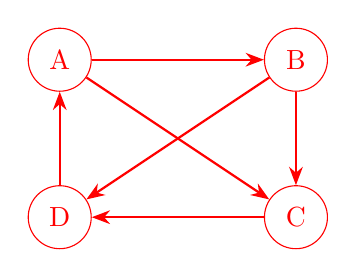
\begin{tikzpicture}[
            node/.style={circle, draw, minimum size=0.8cm},
            arrow/.style={-Stealth, thick}
          ]
          % Define the nodes
          \node[node, red] (A) at (0,0) {A};
          \node[node, red] (B) at (3,0) {B};
          \node[node, red] (C) at (3,-2) {C};
          \node[node, red] (D) at (0,-2) {D};

          % Connect the nodes with directed edges
          \draw[arrow, red] (A) -- (B);
          \draw[arrow, red] (B) -- (C);
          \draw[arrow, red] (C) -- (D);
          \draw[arrow, red] (D) -- (A);
          \draw[arrow, red] (A) -- (C);
          \draw[arrow, red] (B) -- (D);
        \end{tikzpicture}
        \caption{You continue exploring from $B$. There are no more nodes to explore, so you go back to the node you came from $A$. You see that the only remaining neighbor to explore is $C$, but it is already in visited, so you don't need to explore it. You are done.}
      \end{subfigure}

      \caption{Walkthrough of DFS on a small graph. The iterative and recursive approaches are identical.}
      \label{fig:dfs_example}
    \end{figure}
  \end{example}

  \begin{theorem}[Runtime of DFS]
    The runtime of DFS is $O(n+m)$. 
  \end{theorem}
  \begin{proof}
    The runtime complexity of this search is $O(N + M)$ because first, the while loop loops at most over the $N$ nodes. The for loop may loop over $M$ edges, but this is a bit pessemistic in bound. Rather, we can view it as looping over neighbors of each node at most exactly once, and so it considers every edge twice, meaning that the for loop will get called $2M$ times in the entire algorithm. So $N + 2M = O(N + M)$. 
  \end{proof}

  \begin{example}[DFS in a Maze]
    We can represent a grid graph, like a maze, with a two dimensional array that stores whether it is connected north, east, south, and west, where boolean of true represents that there is a wall, and false means there isn't a wall (so connected). 

    \begin{figure}[H]
      \centering
      \begin{subfigure}[b]{0.48\textwidth}
      \centering
        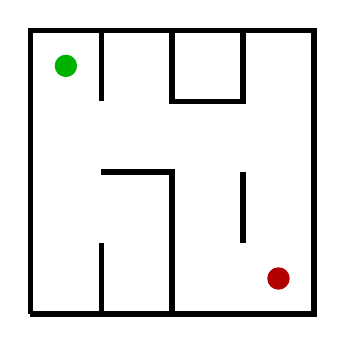
\begin{tikzpicture}[scale=0.9]
          % Outer boundary
          \draw[line width=2pt] (0,0) -- (4,0) -- (4,4) -- (0,4) -- (0,0);
          
          % Internal walls
          % Top section
          \draw[line width=2pt] (1,4) -- (1,3);
          \draw[line width=2pt] (2,4) -- (2,3) -- (3,3) -- (3,4);
          
          % Middle section
          \draw[line width=2pt] (1,2) -- (2,2) -- (2,1);
          \draw[line width=2pt] (3,2) -- (3,1);
          
          % Bottom section
          \draw[line width=2pt] (1,1) -- (1,0);
          \draw[line width=2pt] (2,1) -- (2,0);
          
          % Entry and exit points (just colored circles)
          \filldraw[green!70!black] (0.5,3.5) circle (0.15);
          \filldraw[red!70!black] (3.5,0.5) circle (0.15);
        \end{tikzpicture}
        \caption{4×4 maze representation}
        \label{fig:maze}
      \end{subfigure}
      \hfill 
      \begin{subfigure}[b]{0.48\textwidth}
      \centering
        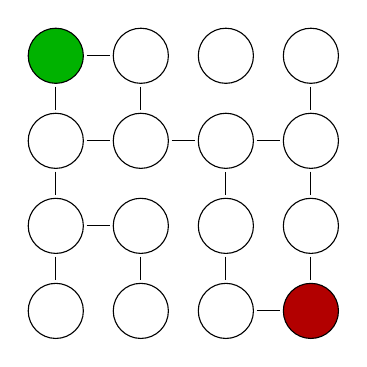
\begin{tikzpicture}[
          scale=0.9,
          node/.style={circle, draw, minimum size=0.7cm},
          edge/.style={draw, -, shorten >=1pt, shorten <=1pt}
        ]
          % Create a 4x4 graph for the new maze
          % Top row
          \node[node, fill=green!70!black, text=white] (A) at (0,3.6) {};
          \node[node] (B) at (1.2,3.6) {};
          \node[node] (C) at (2.4,3.6) {};
          \node[node] (D) at (3.6,3.6) {};
          
          % Second row
          \node[node] (E) at (0,2.4) {};
          \node[node] (F) at (1.2,2.4) {};
          \node[node] (G) at (2.4,2.4) {};
          \node[node] (H) at (3.6,2.4) {};
          
          % Third row
          \node[node] (I) at (0,1.2) {};
          \node[node] (J) at (1.2,1.2) {};
          \node[node] (K) at (2.4,1.2) {};
          \node[node] (L) at (3.6,1.2) {};
          
          % Bottom row
          \node[node] (M) at (0,0) {};
          \node[node] (N) at (1.2,0) {};
          \node[node] (O) at (2.4,0) {};
          \node[node, fill=red!70!black, text=white] (P) at (3.6,0) {};
          
          % Add edges based on available paths in the maze
          % Vertical connections
          \draw[edge] (A) -- (E);
          \draw[edge] (E) -- (I);
          \draw[edge] (I) -- (M);
          \draw[edge] (G) -- (H);
          
          \draw[edge] (B) -- (F);
          
          \draw[edge] (D) -- (H);
          \draw[edge] (H) -- (L);
          \draw[edge] (L) -- (P);
          
          \draw[edge] (J) -- (N);
          
          % Horizontal connections
          \draw[edge] (A) -- (B);
          
          \draw[edge] (E) -- (F);
          \draw[edge] (F) -- (G);
          \draw[edge] (K) -- (G);
          \draw[edge] (K) -- (O);
          
          \draw[edge] (I) -- (J);
          
          \draw[edge] (O) -- (P);
        \end{tikzpicture}
        \caption{Graph representation of the maze.}
        \label{fig:maze-graph}
      \end{subfigure}
      \caption{A 4×4 maze (left) and its corresponding graph representation (right). Start and end points are shown in green and red respectively.}
      \label{fig:maze-and-graph}
    \end{figure}

    But remember that in a tree traversal, we recursively searched down and down until we hit a null node, in which case we backtrack up to look in another branch. For graphs, this is a bit more complicated, since we could go in loops. Therefore, we want to keep track of all the visited nodes to avoid infinite recursion. We have three base cases: 
    \begin{enumerate}
      \item If we search off the grid, then this is not a valid path 
      \item If we already explored here, then we don't want to repeat it 
      \item If we reached the goal of the maze, then we output the length of the path. 
    \end{enumerate}
    The recursive case would take each node and recurse on its 4 adjacent neighbors, if they are connected. Note that this algorithm recurses on each of the $N$ nodes $4$ times (for each direction, and each recursive call is $O(1)$), so the complexity is $O(N)$. 
  \end{example}

  Note that the main idea of DFS is to always explore a new adjacent vertex if possible, and if not, then backtrack to the most recent vertex adjacent to an unvisited vertex and continue. On the contrary, the main idea of BFS is to explore \textit{all} your neighbors before you visit any of your neighbors' neighbors. It exhaustively searches for the closest regions of your search space before you look any further. Unlike DFS, which finds the some arbitrary path to a node, BFS finds the shortest (perhaps non-unique) path to a node. This can be simply done with a queue. 

  \begin{algo}[Iterative Breadth-First Search]
    Breadth-First Search (BFS) explores a graph by visiting all neighbors at the current depth before moving to nodes at the next depth level. It uses a queue to process nodes in the order they are discovered.
    \begin{algorithm}[H]
      \label{alg:bfs}
      \begin{algorithmic}[1]
        \Require{Graph $G(V, E)$, start vertex $s$}
        
        \Function{BFS}{$G, s$}
          \State visited $\gets \emptyset$ \Comment{Initialize empty set of visited vertices}
          \State queue $\gets$ empty queue
          \State Enqueue $s$ onto queue
          \State Add $s$ to visited
          
          \While{queue is not empty}
            \State $u \gets$ Dequeue from queue \Comment{Get the next vertex to process}
            \State \textit{/* Process vertex $u$ here */}
            
            \For{each neighbor $v$ of $u$ in $G$}
              \If{$v \notin$ visited}
                \State Add $v$ to visited
                \State Enqueue $v$ onto queue
              \EndIf
            \EndFor
          \EndWhile
        \EndFunction
      \end{algorithmic}
    \end{algorithm}
  \end{algo}

  \begin{example}[BFS Walkthrough]
    Let's conduct BFS on the following graph. 

    \begin{figure}[H]
      \centering
      \begin{subfigure}[b]{0.48\textwidth}
        \centering
        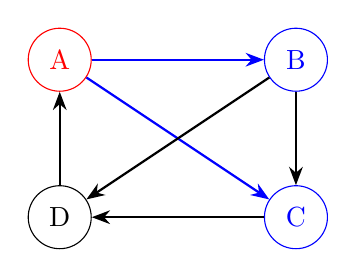
\begin{tikzpicture}[
            node/.style={circle, draw, minimum size=0.8cm},
            arrow/.style={-Stealth, thick}
          ]
          % Define the nodes
          \node[node, red] (A) at (0,0) {A};
          \node[node, blue] (B) at (3,0) {B};
          \node[node, blue] (C) at (3,-2) {C};
          \node[node] (D) at (0,-2) {D};
          % Connect the nodes with directed edges
          \draw[arrow, blue] (A) -- (B);
          \draw[arrow] (B) -- (C);
          \draw[arrow] (C) -- (D);
          \draw[arrow] (D) -- (A);
          \draw[arrow, blue] (A) -- (C);
          \draw[arrow] (B) -- (D);
        \end{tikzpicture}
        \caption{You start at $A$ and you add it to your visited set $V = \{A\}$ and to your queue $[A]$. You immediately dequeue $A$ from the queue and look at all neighbors of $A$, which are $B$ and $C$. You add both to your queue in some random order, say $B$ first. }
      \end{subfigure}
      \hfill 
      \begin{subfigure}[b]{0.48\textwidth}
        \centering
        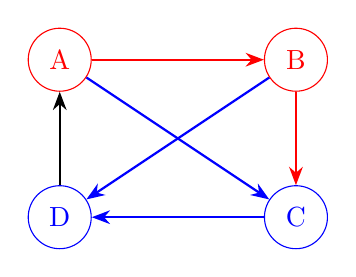
\begin{tikzpicture}[
            node/.style={circle, draw, minimum size=0.8cm},
            arrow/.style={-Stealth, thick}
          ]
          % Define the nodes
          \node[node, red] (A) at (0,0) {A};
          \node[node, red] (B) at (3,0) {B};
          \node[node, blue] (C) at (3,-2) {C};
          \node[node, blue] (D) at (0,-2) {D};
          % Connect the nodes with directed edges
          \draw[arrow, red] (A) -- (B);
          \draw[arrow, red] (B) -- (C);
          \draw[arrow, blue] (C) -- (D);
          \draw[arrow] (D) -- (A);
          \draw[arrow, blue] (A) -- (C);
          \draw[arrow, blue] (B) -- (D);
        \end{tikzpicture}
        \caption{You deque $B$ and see that the adjacent nodes are $C$ and $D$. $C$ is already in your queue (check with visited set, which is $O(1)$), so you do not put it into your queue and can mark the corresponding edges as explored. You do put $D$ into the queue.}
      \end{subfigure}
      \begin{subfigure}[b]{0.48\textwidth}
        \centering
        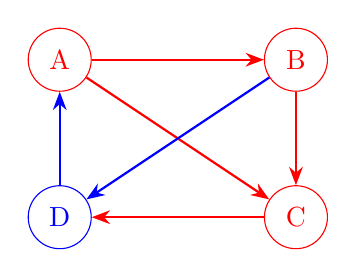
\begin{tikzpicture}[
            node/.style={circle, draw, minimum size=0.8cm},
            arrow/.style={-Stealth, thick}
          ]
          % Define the nodes
          \node[node, red] (A) at (0,0) {A};
          \node[node, red] (B) at (3,0) {B};
          \node[node, red] (C) at (3,-2) {C};
          \node[node, blue] (D) at (0,-2) {D};
          % Connect the nodes with directed edges
          \draw[arrow, red] (A) -- (B);
          \draw[arrow, red] (B) -- (C);
          \draw[arrow, red] (C) -- (D);
          \draw[arrow, blue] (D) -- (A);
          \draw[arrow, red] (A) -- (C);
          \draw[arrow, blue] (B) -- (D);
        \end{tikzpicture}
        \caption{Next you dequeue $C$ since this is first seen from $A$. You explore from here and look at the neighbors, which is $D$. However, $D$ is already in your queue from $B$, so you skip it. There are no more neighbors to explore from $C$, so we look at the queue again.}
      \end{subfigure}
      \hfill 
      \begin{subfigure}[b]{0.48\textwidth}
        \centering
        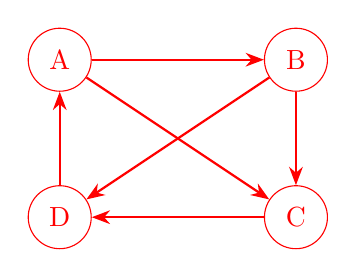
\begin{tikzpicture}[
            node/.style={circle, draw, minimum size=0.8cm},
            arrow/.style={-Stealth, thick}
          ]
          % Define the nodes
          \node[node, red] (A) at (0,0) {A};
          \node[node, red] (B) at (3,0) {B};
          \node[node, red] (C) at (3,-2) {C};
          \node[node, red] (D) at (0,-2) {D};
          % Connect the nodes with directed edges
          \draw[arrow, red] (A) -- (B);
          \draw[arrow, red] (B) -- (C);
          \draw[arrow, red] (C) -- (D);
          \draw[arrow, red] (D) -- (A);
          \draw[arrow, red] (A) -- (C);
          \draw[arrow, red] (B) -- (D);
        \end{tikzpicture}
        \caption{You dequeue $D$ and look at the neighbors. The only neighbor is $A$ and it is already in visited, so we can skip this and mark the corresponding edge as explored. Since there are no more nodes to explore in our queue, this concludes BFS.}
      \end{subfigure}
      \caption{Walkthrough of BFS on a small graph. Blue represents the nodes/edges that are in our queue and red represents the nodes/edges that we have finished exploring.}
      \label{fig:bfs_example}
    \end{figure}
  \end{example}


  \begin{theorem}[Runtime of BFS]
    The runtime of BFS is $O(n+m)$. 
  \end{theorem}
  \begin{proof}
    To get the running time, we know that each vertex is popped only once from the queue, giving us $O(n)$. For each pop, we are exploring all the neighbors of $V$. 
    \begin{align}
      O \bigg( \sum_{v \in V} | \text{neighbors of } v| + 1\bigg) & = O \bigg( \sum_{v \in V} d_v + 1 \bigg) \\
                                           & = O (2 |E| + |V|) = O(m + n )
    \end{align}
    which is linear in input size!  
  \end{proof}

  The more straightforward application is in reachability. 

  \begin{example}[Reachability]
    Given a directed graph and a node $v$, find all nodes that are reachable from $v$. 
  \end{example}

  \begin{definition}[Search Trees]
    Once we have traversed a graph using BFS or DFS, we can label the directed path that this traversal algorithm takes into a \textbf{search tree}. 

    \begin{figure}[H]
      \centering
      \begin{subfigure}[b]{0.48\textwidth}
      \centering
        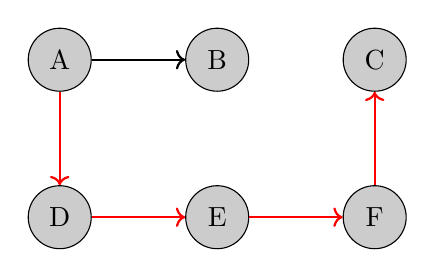
\begin{tikzpicture}[
            node/.style={circle, draw, fill=gray!40, minimum size=0.8cm},
            edge/.style={->, thick}
        ]
        % Create nodes
        \node[node] (A1) at (0,2) {A};
        \node[node] (B1) at (2,2) {B};
        \node[node] (C1) at (4,2) {C};
        \node[node] (D1) at (0,0) {D};
        \node[node] (E1) at (2,0) {E};
        \node[node] (F1) at (4,0) {F};
        
        % Create edges
        \draw[edge] (A1) -- (B1);
        \draw[edge, red, thick] (A1) -- (D1);
        \draw[edge, red, thick] (D1) -- (E1);
        \draw[edge, red, thick] (E1) -- (F1);
        \draw[edge, red, thick] (F1) -- (C1);
        \end{tikzpicture}
        \caption{After DFS traversal, we can store the previous nodes in a hashmap $\{B \mapsto A, D \mapsto A, E \mapsto D, F \mapsto E, C \mapsto F\}$. From this we can see the path to get to $C$ is $A \mapsto D \mapsto E \mapsto F \mapsto C$ of length 4. }
        \label{fig:graph1}
      \end{subfigure}
      \hfill 
      \begin{subfigure}[b]{0.48\textwidth}
      \centering
        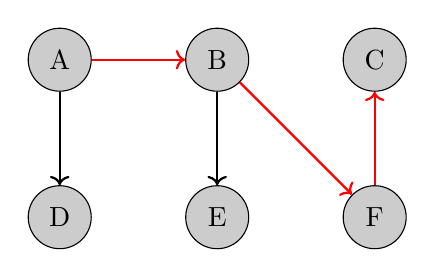
\begin{tikzpicture}[
            node/.style={circle, draw, fill=gray!40, minimum size=0.8cm},
            edge/.style={->, thick}
        ]
        % Create nodes
        \node[node] (A2) at (0,2) {A};
        \node[node] (B2) at (2,2) {B};
        \node[node] (C2) at (4,2) {C};
        \node[node] (D2) at (0,0) {D};
        \node[node] (E2) at (2,0) {E};
        \node[node] (F2) at (4,0) {F};
        
        % Create edges
        \draw[edge, red, thick] (A2) -- (B2);
        \draw[edge] (A2) -- (D2);
        \draw[edge] (B2) -- (E2);
        \draw[edge, red, thick] (B2) -- (F2);
        \draw[edge, red, thick] (F2) -- (C2);
        \end{tikzpicture}
        \caption{After BFS traversal, we can store the previous nodes in a hashmap $\{B \mapsto A, D \mapsto A, E \mapsto B, F \mapsto B, C \mapsto F\}$. From this we can see the path to get to $C$ is $A \mapsto B \mapsto F \mapsto C$ of length 3. }
        \label{fig:graph2}
      \end{subfigure}
      \caption{Comparison of two directed graphs with different path lengths from A to C.}
      \label{fig:graph-comparison}
    \end{figure}

    By construction, we can see that the path from A to C is always shorter for BFS than for DFS. 
  \end{definition}

\subsection{Trees} 

  Now we look at one special type of graph, called a \textit{tree}. 

  \begin{definition}[Trees]
    An undirected graph $G(V, E)$ is a \textbf{tree} iff $G$ is connected and has no cycles.\footnote{ Removing the first requirement gives us the definition of a \textbf{forest}, which is a collection of trees. }
    \begin{enumerate}
      \item The \textbf{root} of the tree is the top node. 
      \item The \textbf{leaf} of the tree are nodes that do not have children. 
      \item A \textbf{path} is any path from one node to another node. A simple path is a path that doesn't cross the same edge twice 
      \item The \textbf{height} of a node is the length of the longest downward path to a leaf from that node. 
      \item The \textbf{depth} of a node is the number of edges from the root to the node. 
      \item The \textbf{size} of the tree is the number of nodes $n$ it contains. 
    \end{enumerate}
  \end{definition}

  \begin{theorem}[Properties of Trees]
    If $G(V, E)$ is a tree, then 
    \begin{enumerate}
      \item There exists a $v \in V$ s.t. $d_v = 1$, called a \textbf{leaf node}. 
      \item $|E| = |V| - 1 = n - 1$. 
    \end{enumerate}
  \end{theorem}
  \begin{proof}
    The outlines are quite intuitive. 
    \begin{enumerate}
      \item There must be some leaf node since if there wasn't, then we would have a cycle. We can use proof by contradiction. 
      \item We can use proof by induction. We start off with one vertex and to construct a tree, we must add one edge and one vertex at every step, keeping this invariant.  
    \end{enumerate}
  \end{proof} 

  Now we can get to the elementary operations on a tree. 

  \begin{algo}[Insert Node to Tree] 
    Inserting is a bit ambiguous since we most also know \textit{where} to insert the value to. In general traversing this tree is $O(\log{n})$, and so we have the same runtime. 
    \begin{algorithmic}[1]
    \Procedure{Insert}{$root, key, value$}
      \If{$root = \text{null}$}
        \State \Return \text{new Node}$(key, value)$
      \EndIf
      \If{$key < root.key$}
        \State $root.left \gets \Call{Insert}{root.left, key, value}$
      \ElsIf{$key > root.key$}
        \State $root.right \gets \Call{Insert}{root.right, key, value}$
      \Else
        \State $root.value \gets value$ \Comment{Update if key already exists}
      \EndIf
      \State \Return $root$
    \EndProcedure
    \end{algorithmic}
  \end{algo}

  \begin{algo}[Remove Node in Tree]
    Removing is very similar, with also a runtime of $O(\log{n})$. 
    \begin{algorithmic}[1]
    \Procedure{Remove}{$root, key$}
      \If{$root = \text{null}$}
        \State \Return $\text{null}$
      \EndIf
      \If{$key < root.key$}
        \State $root.left \gets \Call{Remove}{root.left, key}$
      \ElsIf{$key > root.key$}
        \State $root.right \gets \Call{Remove}{root.right, key}$
      \Else \Comment{Node with the key found}
        \If{$root.left = \text{null}$}
          \State \Return $root.right$
        \ElsIf{$root.right = \text{null}$}
          \State \Return $root.left$
        \EndIf
        \State $root.key \gets \Call{FindMin}{root.right}$
        \State $root.right \gets \Call{Remove}{root.right, root.key}$
      \EndIf
      \State \Return $root$
    \EndProcedure
    \end{algorithmic}
  \end{algo}

  \begin{algo}[Modify Node in Tree]
    Same with modifying a node: $O(\log{n})$. 
    \begin{algorithmic}[1]
    \Procedure{Modify}{$root, key, newValue$}
      \If{$root = \text{null}$}
        \State \Return $\text{null}$ \Comment{Key not found}
      \EndIf
      \If{$key < root.key$}
        \State $root.left \gets \Call{Modify}{root.left, key, newValue}$
      \ElsIf{$key > root.key$}
        \State $root.right \gets \Call{Modify}{root.right, key, newValue}$
      \Else
        \State $root.value \gets newValue$ \Comment{Update value when key is found}
      \EndIf
      \State \Return $root$
    \EndProcedure
    \end{algorithmic}
  \end{algo}

  Since a node also has a specified depth and height, we should also know how to calculate this. 

  \begin{algo}[Height of Node]
    The height of a node is the longest downward path to a leaf from that node, so its height would be the maximum of the two heights of its children. A null node would have height $-1$, which is our base case. 
    \begin{algorithmic}[1]
    \Procedure{GetHeight}{$root$}
      \If{$root = \text{null}$}
        \State \Return $-1$
      \EndIf
      \State \Return $1 + \max(\Call{GetHeight}{root.\text{left}}, \Call{GetHeight}{root.\text{right}})$
    \EndProcedure
    \end{algorithmic}
  \end{algo}

  \begin{algo}[Depth of Node]
    The depth is quite hard to find recursively, but if we have a reference to the parent, then we can write 
    \begin{algorithmic}[1]
    \Procedure{Depth}{$node$}
      \If{$node = \text{null}$}
        \State \Return $-1$
      \Else
        \State \Return $1 + \Call{Depth}{node.\text{parent}}$
      \EndIf
    \EndProcedure
    \end{algorithmic}
  \end{algo}

\subsubsection{Binary Trees} 

  Most of the time, we work with \textit{binary trees}, which means that each node has has at most 2 children, denoted a \textit{left child} and \textit{right child}. 

  \begin{definition}[Binary Tree]
    A \textbf{binary tree} is a recursive data structure in which every node has up to two children, which we call the \textbf{left child} and \textbf{right child}. 

    \begin{figure}[H]
      \centering 
      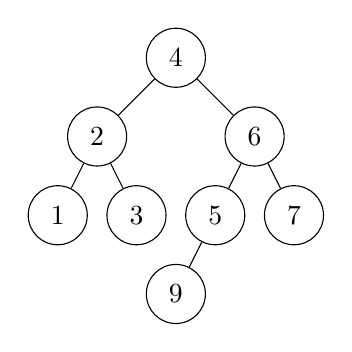
\begin{tikzpicture}[  every node/.style={    circle,    minimum size=0.75cm,    draw,    text centered,    anchor=center  }]
        \node (4) at (0,0) {4};
        \node (2) at (-1,-1) {2};
        \node (6) at (1,-1) {6};
        \node (1) at (-1.5,-2) {1};
        \node (3) at (-0.5,-2) {3};
        \node (5) at (0.5,-2) {5};
        \node (7) at (1.5,-2) {7};
        \node (9) at (0, -3) {9}; 
        \draw (4) -- (2);
        \draw (4) -- (6);
        \draw (2) -- (1);
        \draw (2) -- (3);
        \draw (6) -- (5);
        \draw (6) -- (7); 
        \draw (5) -- (9); 
      \end{tikzpicture}
      \caption{An example of a binary tree. The root is 4, with a max depth of 3. } 
      \label{fig:binary_tree}
    \end{figure}
  \end{definition} 

  A natural question is whether we can take this tree structure and retrieve all of its values. There are three recursive paradigms to do this, which differs by where the nonrecursive call is. 

  \begin{algo}[In Order Traversal]
    \textbf{In-Order traversal} tells us to print everything on the left of the node, then print the node, and then print everything on the right. 
    \begin{algorithmic}[1]
    \Procedure{InOrder}{$t$}
      \If{$t \neq \text{null}$}
        \State \Call{InOrder}{$t.\text{left}$}
        \State \textbf{print} $t.\text{info}$
        \State \Call{InOrder}{$t.\text{right}$}
      \EndIf
    \EndProcedure
    \end{algorithmic}
  \end{algo}

  \begin{algo}[PreOrder Traversal]
    \textbf{Pre-Order traversal} tells us to print the node itself first, then print all the ones on the left, and then print all the ones on the right. 
    \begin{algorithmic}[1]
    \Procedure{PreOrder}{$t$}
      \If{$t \neq \text{null}$}
        \State \textbf{print} $t.\text{info}$
        \State \Call{PreOrder}{$t.\text{left}$}
        \State \Call{PreOrder}{$t.\text{right}$}
      \EndIf
    \EndProcedure
    \end{algorithmic}
  \end{algo}

  \begin{algo}[PostOrder Traversal]
    \textbf{Post-Order traversal} tells us to print all the nodes on the left, then all ones on the right, and then the node itself. 
    \begin{algorithmic}[1]
    \Procedure{PostOrder}{$t$}
      \If{$t \neq \text{null}$}
        \State \Call{PostOrder}{$t.\text{left}$}
        \State \Call{PostOrder}{$t.\text{right}$}
        \State \textbf{print} $t.\text{info}$
      \EndIf
    \EndProcedure
    \end{algorithmic}
  \end{algo} 

  \begin{example}[Converting Tree to List]
    It's worth to go over an example here. Given the following binary tree, 

    \begin{figure}[H]
      \centering 
      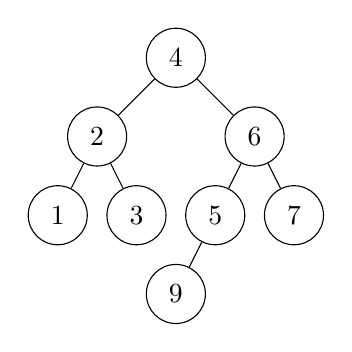
\begin{tikzpicture}[  every node/.style={    circle,    minimum size=0.75cm,    draw,    text centered,    anchor=center  }]
        \node (4) at (0,0) {4};
        \node (2) at (-1,-1) {2};
        \node (6) at (1,-1) {6};
        \node (1) at (-1.5,-2) {1};
        \node (3) at (-0.5,-2) {3};
        \node (5) at (0.5,-2) {5};
        \node (7) at (1.5,-2) {7};
        \node (9) at (0, -3) {9}; 
        \draw (4) -- (2);
        \draw (4) -- (6);
        \draw (2) -- (1);
        \draw (2) -- (3);
        \draw (6) -- (5);
        \draw (6) -- (7); 
        \draw (5) -- (9); 
      \end{tikzpicture}
      \caption{An example of a binary tree. The root is 4, with a max depth of 3. } 
      \label{fig:binary_tree_to_list}
    \end{figure}
    If we initialize a list and replace the print statement with an insert to the (end of the) list, then 
    \begin{enumerate}
      \item a in-order traversal produces: $[1, 2, 3, 4, 9, 5, 6, 7]$
      \item a pre-order traversal produces: $[4, 2, 1, 3, 6, 5, 9, 7]$
      \item a post-order traversal produces: $[1, 3, 2, 9, 5, 7, 6, 4]$
    \end{enumerate}
  \end{example}

  What we have described is a traversal method, and a natural question is to ask: Are these related to the more general DFS and BFS in any way? In fact it is. 

  \begin{theorem}[Tree Traversals and DFS]
    All forms of traversal are a specific variant of DFS starting from the root. 
    \begin{enumerate}
      \item A pre-order traversal prioritizes the left node to explore and is the common DFS variant used in general graph traversal.  
      \item An in-order traversal always prioritizes adding an unexplored left child to the stack, and if there is no left child, then the node is printed, and then the right child is pushed to the stack and explored. 
      \item A post-order traversal always prioritizes adding an unexplored left child to the stack, and if there is no left child, then the right child is pushed to the stack and explored. Once the right child is finished exploring the parent node is printed. 
    \end{enumerate}
  \end{theorem}

  So what does BFS do? There is another traversal which traverses the layers of each tree. 

  \begin{algo}[Level Order Traversal]
    \textbf{Level-order traversal} tells us to print all nodes of depth $0$, then all nodes of depth $1$, and so on.
    \begin{algorithmic}[1]
    \Procedure{LevelOrder}{$t$}
      \If{$t \neq \text{null}$}
        \State Create an empty queue $Q$
        \State Enqueue $t$ to $Q$
        \While{$Q$ is not empty}
          \State $node \gets$ Dequeue from $Q$
          \State \textbf{print} $node.\text{info}$
          \If{$node.\text{left} \neq \text{null}$}
            \State Enqueue $node.\text{left}$ to $Q$
          \EndIf
          \If{$node.\text{right} \neq \text{null}$}
            \State Enqueue $node.\text{right}$ to $Q$
          \EndIf
        \EndWhile
      \EndIf
    \EndProcedure
    \end{algorithmic}
  \end{algo}

\subsection{Heaps}

  A heap is sort of in between a sorted array and an unsorted array. 

  \begin{definition}[Binary Heap]
    A \textbf{binary heap} is a binary tree satisfying the following structural invariants: 
    \begin{enumerate}
      \item Maintain the \textbf{heap property} that every node is less than or equal to its successors, and 
      \item The \textbf{shape property} that the tree is complete (full except perhaps last level, in which case it should be filled from left to right. 
    \end{enumerate}

    \begin{figure}[H]
      \centering
      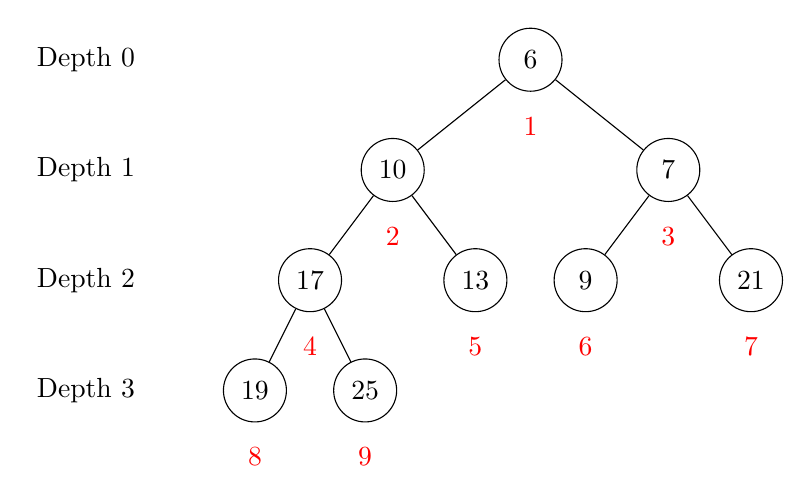
\begin{tikzpicture}[scale=0.7]
        \node[left] at (-2,0) {Depth 0};
        \node[left] at (-2,-2) {Depth 1};
        \node[left] at (-2,-4) {Depth 2};
        \node[left] at (-2,-6) {Depth 3};
        
        % Nodes
        % Depth 0
        \node[circle, draw, minimum size=0.8cm] (n1) at (5,0) {6};
        \node[below=0.2cm of n1, red] {1};
        
        % Depth 1
        \node[circle, draw, minimum size=0.8cm] (n2) at (2.5,-2) {10};
        \node[below=0.2cm of n2, red] {2};
        \node[circle, draw, minimum size=0.8cm] (n3) at (7.5,-2) {7};
        \node[below=0.2cm of n3, red] {3};
        
        % Depth 2
        \node[circle, draw, minimum size=0.8cm] (n4) at (1,-4) {17};
        \node[below=0.2cm of n4, red] {4};
        \node[circle, draw, minimum size=0.8cm] (n5) at (4,-4) {13};
        \node[below=0.2cm of n5, red] {5};
        \node[circle, draw, minimum size=0.8cm] (n6) at (6,-4) {9};
        \node[below=0.2cm of n6, red] {6};
        \node[circle, draw, minimum size=0.8cm] (n7) at (9,-4) {21};
        \node[below=0.2cm of n7, red] {7};
        
        % Depth 3
        \node[circle, draw, minimum size=0.8cm] (n8) at (0,-6) {19};
        \node[below=0.2cm of n8, red] {8};
        \node[circle, draw, minimum size=0.8cm] (n9) at (2,-6) {25};
        \node[below=0.2cm of n9, red] {9};
        
        % Edges
        \draw (n1) -- (n2);
        \draw (n1) -- (n3);
        \draw (n2) -- (n4);
        \draw (n2) -- (n5);
        \draw (n3) -- (n6);
        \draw (n3) -- (n7);
        \draw (n4) -- (n8);
        \draw (n4) -- (n9);
      \end{tikzpicture}
      \caption{Tree structure of a binary heap, with red labels representing the indices of the array structure mentioned below. }
      \label{fig:binary-heap}
    \end{figure}
  \end{definition}

  We should conceptually think of a binary heap as an underlying binary tree, but it is actually usually implemented with an array, and we can create a map from the heap to the array with the following indices. 

  \begin{figure}[H]
    \centering 
    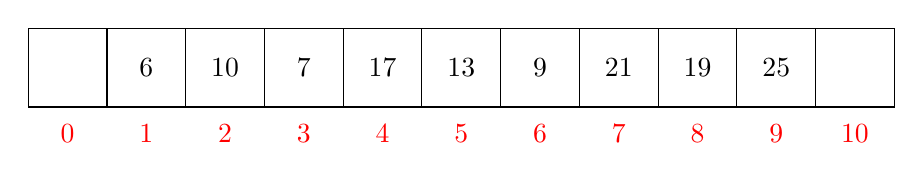
\begin{tikzpicture}
      \foreach \i in {0,...,10} {
        \draw (\i,0) rectangle +(1,1);
        \node[below] at (\i+0.5,-0.1) {\textcolor{red}{\i}};
      }
      
      % Add the values
      \node at (1.5,0.5) {6};
      \node at (2.5,0.5) {10};
      \node at (3.5,0.5) {7};
      \node at (4.5,0.5) {17};
      \node at (5.5,0.5) {13};
      \node at (6.5,0.5) {9};
      \node at (7.5,0.5) {21};
      \node at (8.5,0.5) {19};
      \node at (9.5,0.5) {25};
    \end{tikzpicture}
    \caption{When 1-indexing, for node with index $k$, the left child is index $2k$, the right child is index $2k + 1$, and the parent is index $k/2$ (where this is integer division). } 
    \label{fig:binary_heap_array}
  \end{figure}

  Implementing peek is easy, since we just return the first index, but it can be quite tricky to maintain this invariant after an arbitrary sequence of add/remove operations. 
  \begin{enumerate}
    \item To add values to a heap, we add to the first open position in the last level of the tree (to maintain the shape property), and then swap with the parent is the heap property is violated. If we are swapping with the parent at most $\log(N)$ times, then the add property has $O(\log(N))$ complexity. 

    \begin{figure}[H]
      \centering
      \begin{subfigure}[b]{0.48\textwidth}
      \centering
        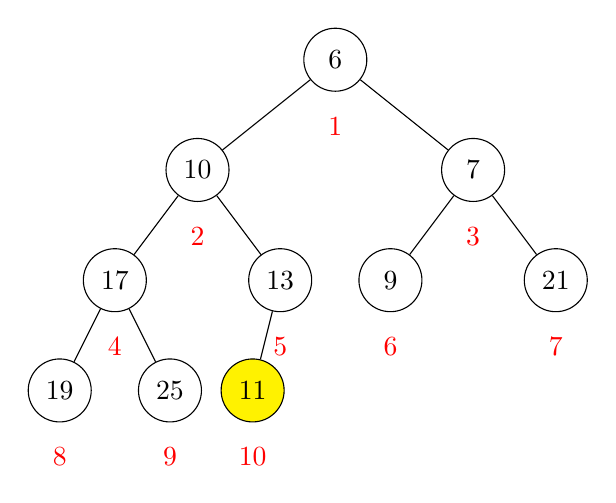
\begin{tikzpicture}[scale=0.7]
          % Nodes
          % Depth 0
          \node[circle, draw, minimum size=0.8cm] (n1) at (5,0) {6};
          \node[below=0.2cm of n1, red] {1};
          
          % Depth 1
          \node[circle, draw, minimum size=0.8cm] (n2) at (2.5,-2) {10};
          \node[below=0.2cm of n2, red] {2};
          \node[circle, draw, minimum size=0.8cm] (n3) at (7.5,-2) {7};
          \node[below=0.2cm of n3, red] {3};
          
          % Depth 2
          \node[circle, draw, minimum size=0.8cm] (n4) at (1,-4) {17};
          \node[below=0.2cm of n4, red] {4};
          \node[circle, draw, minimum size=0.8cm] (n5) at (4,-4) {13};
          \node[below=0.2cm of n5, red] {5};
          \node[circle, draw, minimum size=0.8cm] (n6) at (6,-4) {9};
          \node[below=0.2cm of n6, red] {6};
          \node[circle, draw, minimum size=0.8cm] (n7) at (9,-4) {21};
          \node[below=0.2cm of n7, red] {7};
          
          % Depth 3
          \node[circle, draw, minimum size=0.8cm] (n8) at (0,-6) {19};
          \node[below=0.2cm of n8, red] {8};
          \node[circle, draw, minimum size=0.8cm] (n9) at (2,-6) {25};
          \node[below=0.2cm of n9, red] {9};
          \node[circle, draw, minimum size=0.8cm, fill=yellow] (n10) at (3.5,-6) {11};
          \node[below=0.2cm of n10, red] {10};
          
          % Edges
          \draw (n1) -- (n2);
          \draw (n1) -- (n3);
          \draw (n2) -- (n4);
          \draw (n2) -- (n5);
          \draw (n3) -- (n6);
          \draw (n3) -- (n7);
          \draw (n4) -- (n8);
          \draw (n4) -- (n9);
          \draw (n5) -- (n10);
        \end{tikzpicture}
        \caption{Add the 11 node to the tree by inserting in the lowest depth, from left to right.}
        \label{fig:first_add}
      \end{subfigure}
      \hfill 
      \begin{subfigure}[b]{0.48\textwidth}
      \centering
        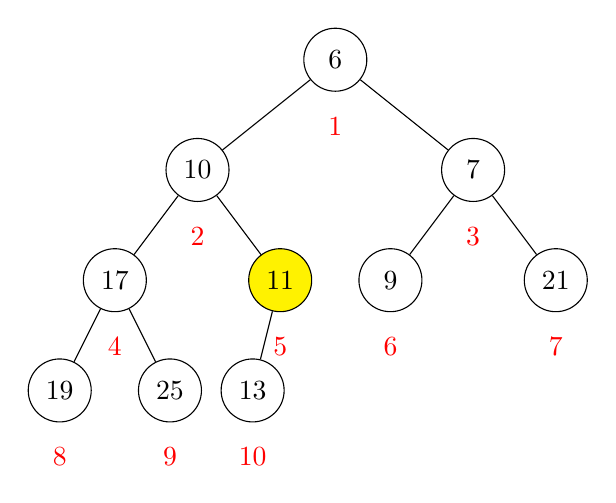
\begin{tikzpicture}[scale=0.7]
          % Nodes
          % Depth 0
          \node[circle, draw, minimum size=0.8cm] (n1) at (5,0) {6};
          \node[below=0.2cm of n1, red] {1};
          
          % Depth 1
          \node[circle, draw, minimum size=0.8cm] (n2) at (2.5,-2) {10};
          \node[below=0.2cm of n2, red] {2};
          \node[circle, draw, minimum size=0.8cm] (n3) at (7.5,-2) {7};
          \node[below=0.2cm of n3, red] {3};
          
          % Depth 2
          \node[circle, draw, minimum size=0.8cm] (n4) at (1,-4) {17};
          \node[below=0.2cm of n4, red] {4};
          \node[circle, draw, minimum size=0.8cm, fill=yellow] (n5) at (4,-4) {11};
          \node[below=0.2cm of n5, red] {5};
          \node[circle, draw, minimum size=0.8cm] (n6) at (6,-4) {9};
          \node[below=0.2cm of n6, red] {6};
          \node[circle, draw, minimum size=0.8cm] (n7) at (9,-4) {21};
          \node[below=0.2cm of n7, red] {7};
          
          % Depth 3
          \node[circle, draw, minimum size=0.8cm] (n8) at (0,-6) {19};
          \node[below=0.2cm of n8, red] {8};
          \node[circle, draw, minimum size=0.8cm] (n9) at (2,-6) {25};
          \node[below=0.2cm of n9, red] {9};
          \node[circle, draw, minimum size=0.8cm] (n10) at (3.5,-6) {13};
          \node[below=0.2cm of n10, red] {10};
          
          % Edges
          \draw (n1) -- (n2);
          \draw (n1) -- (n3);
          \draw (n2) -- (n4);
          \draw (n2) -- (n5);
          \draw (n3) -- (n6);
          \draw (n3) -- (n7);
          \draw (n4) -- (n8);
          \draw (n4) -- (n9);
          \draw (n5) -- (n10);
        \end{tikzpicture}
        \caption{Keep swapping the added node with its ancestor if the node is smaller.}
        \label{fig:then_swap}
      \end{subfigure}
      \caption{Visual of how to add nodes to a heap. }
      \label{fig:head_add}
    \end{figure} 

    \item We remove the first (minimal) value, we first replace the root with the last node in the heap, and while the heap property is violated, we swap with the smaller child. There are two choices, the left or right child, in which we can swap. But we must always swap with the \textbf{smaller child}, since we swapped with the bigger child, then this bigger child would be larger than the smaller one, violating the heap property. Since a complete binary tree always has height $O(\log(N))$, remove also "traverses" one root-leaf path, and so its runtime complexity is $O(\log(N))$, too. hi

    \begin{figure}[H]
      \centering
      \begin{subfigure}[b]{0.48\textwidth}
      \centering
        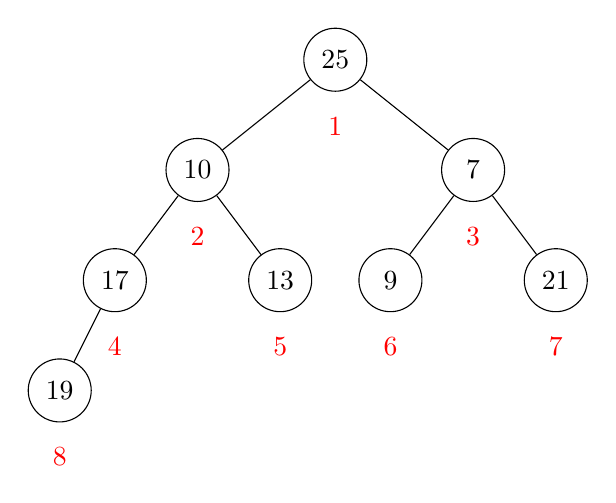
\begin{tikzpicture}[scale=0.7]
          % Nodes
          % Depth 0
          \node[circle, draw, minimum size=0.8cm] (n1) at (5,0) {25};
          \node[below=0.2cm of n1, red] {1};
          
          % Depth 1
          \node[circle, draw, minimum size=0.8cm] (n2) at (2.5,-2) {10};
          \node[below=0.2cm of n2, red] {2};
          \node[circle, draw, minimum size=0.8cm] (n3) at (7.5,-2) {7};
          \node[below=0.2cm of n3, red] {3};
          
          % Depth 2
          \node[circle, draw, minimum size=0.8cm] (n4) at (1,-4) {17};
          \node[below=0.2cm of n4, red] {4};
          \node[circle, draw, minimum size=0.8cm] (n5) at (4,-4) {13};
          \node[below=0.2cm of n5, red] {5};
          \node[circle, draw, minimum size=0.8cm] (n6) at (6,-4) {9};
          \node[below=0.2cm of n6, red] {6};
          \node[circle, draw, minimum size=0.8cm] (n7) at (9,-4) {21};
          \node[below=0.2cm of n7, red] {7};
          
          % Depth 3
          \node[circle, draw, minimum size=0.8cm] (n8) at (0,-6) {19};
          \node[below=0.2cm of n8, red] {8};
          
          % Edges
          \draw (n1) -- (n2);
          \draw (n1) -- (n3);
          \draw (n2) -- (n4);
          \draw (n2) -- (n5);
          \draw (n3) -- (n6);
          \draw (n3) -- (n7);
          \draw (n4) -- (n8);
        \end{tikzpicture}
        \caption{Pop 6 node and replace it with last node 25.}
        \label{fig:remove-heap-step1}
      \end{subfigure}
      \hfill 
      \begin{subfigure}[b]{0.48\textwidth}
      \centering
        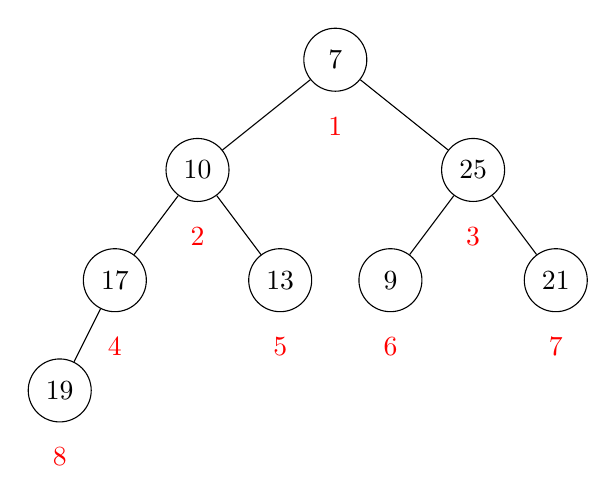
\begin{tikzpicture}[scale=0.7]
          % Nodes
          % Depth 0
          \node[circle, draw, minimum size=0.8cm] (n1) at (5,0) {7};
          \node[below=0.2cm of n1, red] {1};
          
          % Depth 1
          \node[circle, draw, minimum size=0.8cm] (n2) at (2.5,-2) {10};
          \node[below=0.2cm of n2, red] {2};
          \node[circle, draw, minimum size=0.8cm] (n3) at (7.5,-2) {25};
          \node[below=0.2cm of n3, red] {3};
          
          % Depth 2
          \node[circle, draw, minimum size=0.8cm] (n4) at (1,-4) {17};
          \node[below=0.2cm of n4, red] {4};
          \node[circle, draw, minimum size=0.8cm] (n5) at (4,-4) {13};
          \node[below=0.2cm of n5, red] {5};
          \node[circle, draw, minimum size=0.8cm] (n6) at (6,-4) {9};
          \node[below=0.2cm of n6, red] {6};
          \node[circle, draw, minimum size=0.8cm] (n7) at (9,-4) {21};
          \node[below=0.2cm of n7, red] {7};
          
          % Depth 3
          \node[circle, draw, minimum size=0.8cm] (n8) at (0,-6) {19};
          \node[below=0.2cm of n8, red] {8};
          
          % Edges
          \draw (n1) -- (n2);
          \draw (n1) -- (n3);
          \draw (n2) -- (n4);
          \draw (n2) -- (n5);
          \draw (n3) -- (n6);
          \draw (n3) -- (n7);
          \draw (n4) -- (n8);
        \end{tikzpicture}
        \caption{Swap the 25 node with the smaller 7 node.}
        \label{fig:remove-heap-step2}
      \end{subfigure}

      \begin{subfigure}[b]{0.48\textwidth}
      \centering
        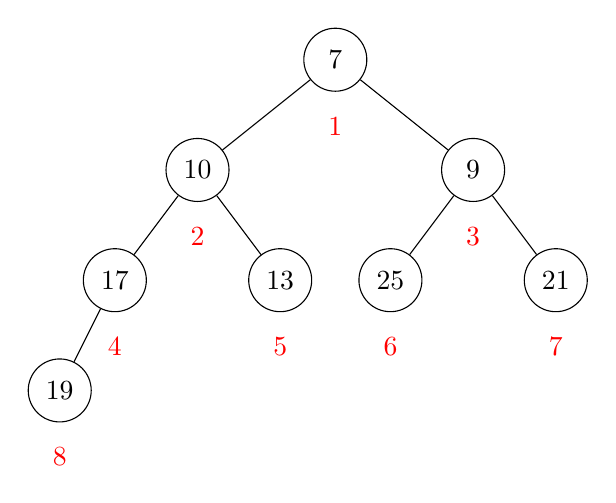
\begin{tikzpicture}[scale=0.7]
          % Nodes
          % Depth 0
          \node[circle, draw, minimum size=0.8cm] (n1) at (5,0) {7};
          \node[below=0.2cm of n1, red] {1};
          
          % Depth 1
          \node[circle, draw, minimum size=0.8cm] (n2) at (2.5,-2) {10};
          \node[below=0.2cm of n2, red] {2};
          \node[circle, draw, minimum size=0.8cm] (n3) at (7.5,-2) {9};
          \node[below=0.2cm of n3, red] {3};
          
          % Depth 2
          \node[circle, draw, minimum size=0.8cm] (n4) at (1,-4) {17};
          \node[below=0.2cm of n4, red] {4};
          \node[circle, draw, minimum size=0.8cm] (n5) at (4,-4) {13};
          \node[below=0.2cm of n5, red] {5};
          \node[circle, draw, minimum size=0.8cm] (n6) at (6,-4) {25};
          \node[below=0.2cm of n6, red] {6};
          \node[circle, draw, minimum size=0.8cm] (n7) at (9,-4) {21};
          \node[below=0.2cm of n7, red] {7};
          
          % Depth 3
          \node[circle, draw, minimum size=0.8cm] (n8) at (0,-6) {19};
          \node[below=0.2cm of n8, red] {8};
          
          % Edges
          \draw (n1) -- (n2);
          \draw (n1) -- (n3);
          \draw (n2) -- (n4);
          \draw (n2) -- (n5);
          \draw (n3) -- (n6);
          \draw (n3) -- (n7);
          \draw (n4) -- (n8);
        \end{tikzpicture}
        \caption{Swap the 25 node with the smaller 9 node.}
        \label{fig:remove-heap-step3}
      \end{subfigure}

      \caption{Binary heap restructuring during deletion operation}
      \label{fig:remove-heap}
    \end{figure}
    
    \item The decreaseKey operation just takes an arbitrary node and decreases its value to some other integer. In this case, it wouldn't violate the shape property, and to restore the heap property, we just put swap it with its parent if the new value is smaller than its parent, making this operation $O(\log(N))$. 
  \end{enumerate}

  \begin{definition}[Priority Queues]
    A priority queue simply adds things according to their priority. Every time we add an element, it looks at where the element should go to keep the list sorted. If we want to dequeue, then we just remove the first element of the list. If we implement a priority queue with a heap, we have
    \begin{enumerate}
      \item Adding a new value is $O(\log N)$. 
      \item Removing a specific value is $O(\log N)$. 
      \item Peek returns the minimal element and is $O(1)$. 
      \item Checking if a value is contained in a priority queue is ?. 
    \end{enumerate}
  \end{definition}

\subsection{Binary Search Trees}

  \begin{definition}[Binary Search Tree]
    A binary tree is a \textbf{binary search tree} if for every node, the left subtree values are all less than the node's value, and the right subtree values are all greater than the node's value. That is, the nodes are in order, and if we called $\texttt{inOrder(root)}$ on the tree, then we would get a sorted list, which allows for efficient search. 
  \end{definition}

  Adding elements to a binary search tree is also very similar. But note that the order in which we add elements to the binary search tree will matter, since it can either make the tree \textbf{balanced} or \textbf{unbalanced}. 

  \begin{figure}[H]
    \centering 
    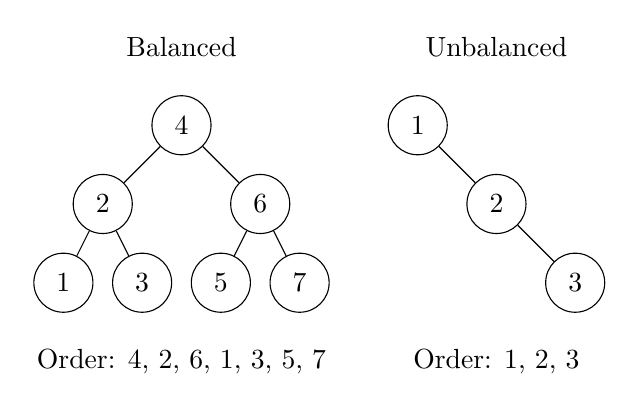
\begin{tikzpicture}[ integer/.style={    draw,    circle,    minimum size=0.75cm,    inner sep=0pt,    text centered,    anchor=center  }]
      % Balanced tree
      \node[integer] (4) at (0,0) {4};
      \node[integer] (2) at (-1,-1) {2};
      \node[integer] (6) at (1,-1) {6};
      \node[integer] (1) at (-1.5,-2) {1};
      \node[integer] (3) at (-0.5,-2) {3};
      \node[integer] (5) at (0.5,-2) {5};
      \node[integer] (7) at (1.5,-2) {7};
      \draw (4) -- (2);
      \draw (4) -- (6);
      \draw (2) -- (1);
      \draw (2) -- (3);
      \draw (6) -- (5);
      \draw (6) -- (7);

      % Caption for balanced tree
      \node at (0,1) {Balanced};
      \node at (0,-3) {Order: 4, 2, 6, 1, 3, 5, 7};

      % Unbalanced tree
      \node[integer] (1') at (3,0) {1};
      \node[integer] (2') at (4,-1) {2};
      \node[integer] (3') at (5,-2) {3};
      \draw (1') -- (2');
      \draw (2') -- (3');

      % Caption for unbalanced tree
      \node at (4,1) {Unbalanced};
      \node at (4,-3) {Order: 1, 2, 3};
    \end{tikzpicture}
    \caption{Comparison of balanced and unbalanced binary trees. In a balanced case, contains/add will be $O(\log(N))$, while in an unbalanced case, we will have $O(N)$.}
    \label{fig:trees}
  \end{figure}

  \begin{definition}[Binary Search]
    Given that we have a sorted list (this is important!), we can search for the index of an element in $O(\log{n})$ time. We want the loop invariant "if the target is in the array/list, it is in the range [low, high]." Let us have a list of $N$ elements, and at every step, we either 
    \begin{enumerate}
      \item get our desired element and its index, or 
      \item cut down our search space by half
    \end{enumerate}
  \end{definition}

  Now, we have learned how we can implement a priority queue using a binary heap. This is also possible to use a binary search tree, since it's easy to get the minimal element for adding and removing, but there are three things that make it difficult: 
  \begin{enumerate}
      \item all elements must be unique 
      \item it is not array-based, and so uses more memory and higher constant factors on runtime 
      \item it is much harder to implement with guarantees that the tree will be balanced. This makes it difficult since if we want to search through a balanced BST, it is $O(\log(N))$, but if it turns out to be unbalanced, then it is $O(N)$. 
  \end{enumerate}
  Therefore, while a balanced tree may be efficient on average, in the worst case the linear complexity is not tolerable. Therefore, we must implement a binary search tree that will do extra work to ensure that they are approximately balanced. This is where \textit{red-black trees}, which are a special type of binary search trees, come in.  

  \begin{definition}[Red-Black Tree]
    \textbf{Red-Black Trees} are binary search trees consisting of nodes that are labeled either red or black that satisfy the following properties: 
    \begin{enumerate}
      \item The root is black 
      \item A red node cannot have red children 
      \item From any node, all paths to null descendants must have the same number of black nodes. (Null is considered to be a black node)
    \end{enumerate}

    \begin{figure}[H]
      \centering
      \begin{subfigure}[b]{0.32\textwidth}
      \centering
        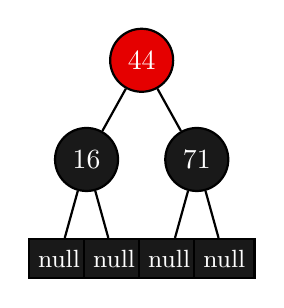
\begin{tikzpicture}[
          scale=0.7,
          red_node/.style={circle, draw, thick, fill=red!90!black, text=white, minimum size=0.8cm},
          black_node/.style={circle, draw, thick, fill=black!90, text=white, minimum size=0.8cm},
          null_node/.style={rectangle, draw, thick, fill=black!90, text=white, minimum size=0.5cm, font=\small},
          edge/.style={draw, thick, -}
        ]
        % First tree (invalid red-black tree)
        % Nodes
        \node[red_node] (n44) at (0,0) {44};
        \node[black_node] (n16) at (-1,-1.8) {16};
        \node[black_node] (n71) at (1,-1.8) {71};
        \node[null_node] (n16l) at (-1.5,-3.6) {null};
        \node[null_node] (n16r) at (-0.5,-3.6) {null};
        \node[null_node] (n71l) at (0.5,-3.6) {null};
        \node[null_node] (n71r) at (1.5,-3.6) {null};
        
        % Edges
        \draw[edge] (n44) -- (n16);
        \draw[edge] (n44) -- (n71);
        \draw[edge] (n16) -- (n16l);
        \draw[edge] (n16) -- (n16r);
        \draw[edge] (n71) -- (n71l);
        \draw[edge] (n71) -- (n71r);
        \end{tikzpicture}
        \caption{Invalid: Root node is red, violating the property that the root must be black.}
        \label{fig:rb-invalid1}
      \end{subfigure}
      \hfill 
      \begin{subfigure}[b]{0.32\textwidth}
      \centering
        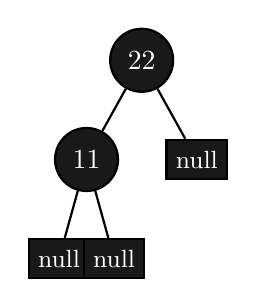
\begin{tikzpicture}[
          scale=0.7,
          red_node/.style={circle, draw, thick, fill=red!90!black, text=white, minimum size=0.8cm},
          black_node/.style={circle, draw, thick, fill=black!90, text=white, minimum size=0.8cm},
          null_node/.style={rectangle, draw, thick, fill=black!90, text=white, minimum size=0.5cm, font=\small},
          edge/.style={draw, thick, -}
        ]
        % Second tree (invalid red-black tree)
        % Nodes
        \node[black_node] (n22) at (0,0) {22};
        \node[black_node] (n11) at (-1,-1.8) {11};
        \node[null_node] (n22r) at (1,-1.8) {null};
        \node[null_node] (n11l) at (-1.5,-3.6) {null};
        \node[null_node] (n11r) at (-0.5,-3.6) {null};
        
        % Edges
        \draw[edge] (n22) -- (n11);
        \draw[edge] (n22) -- (n22r);
        \draw[edge] (n11) -- (n11l);
        \draw[edge] (n11) -- (n11r);
        \end{tikzpicture}
        \caption{Invalid: Path (22,null) has 2 black nodes, but path (22,11,null) has 3, violating the black-depth property.}
        \label{fig:rb-invalid2}
      \end{subfigure}
      \hfill 
      \begin{subfigure}[b]{0.32\textwidth}
      \centering
        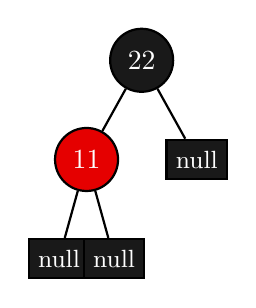
\begin{tikzpicture}[
          scale=0.7,
          red_node/.style={circle, draw, thick, fill=red!90!black, text=white, minimum size=0.8cm},
          black_node/.style={circle, draw, thick, fill=black!90, text=white, minimum size=0.8cm},
          null_node/.style={rectangle, draw, thick, fill=black!90, text=white, minimum size=0.5cm, font=\small},
          edge/.style={draw, thick, -}
        ]
        % Third tree (valid red-black tree)
        % Nodes
        \node[black_node] (n22) at (0,0) {22};
        \node[red_node] (n11) at (-1,-1.8) {11};
        \node[null_node] (n22r) at (1,-1.8) {null};
        \node[null_node] (n11l) at (-1.5,-3.6) {null};
        \node[null_node] (n11r) at (-0.5,-3.6) {null};
        
        % Edges
        \draw[edge] (n22) -- (n11);
        \draw[edge] (n22) -- (n22r);
        \draw[edge] (n11) -- (n11l);
        \draw[edge] (n11) -- (n11r);
        \end{tikzpicture}
        \caption{Valid: Root is black, reds have no red children, all paths from node to null have same black counts.}
        \label{fig:rb-valid}
      \end{subfigure}
      \caption{Examples and non-examples of red-black trees.}
      \label{fig:red-black-tree-examples}
    \end{figure}

    Remember that red black trees are also just binary search trees, and so some of the operations are the same.  
    \begin{enumerate}
      \item contains (search) method is the exact same thing as BST 
      \item The add method needs to be slightly modified, since after we add, we need to make sure that the resulting tree is a red-black tree. This is done in three steps: 
      \begin{enumerate}
        \item Run the regular BST add 
        \item Color the new node red 
        \item Fix the tree to reestablish red-black tree properties. This is extremely complicated with different cases, but it all essentially uses some sort of recoloring and a (right or left) rotation of the tree. 
      \end{enumerate}
    \end{enumerate}
  \end{definition}

  Note that there are binary search trees that cannot be turned into a red-black tree. 

  \begin{figure}[H]
    \centering
    \begin{subfigure}[b]{0.24\textwidth}
    \centering
      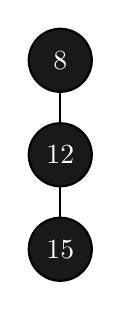
\begin{tikzpicture}[
        scale=0.6,
        red_node/.style={circle, draw, thick, fill=red!90!black, text=white, minimum size=0.8cm},
        black_node/.style={circle, draw, thick, fill=black!90, text=white, minimum size=0.8cm},
        edge/.style={draw, thick, -}
      ]
      % First tree - all black
      % Nodes
      \node[black_node] (n8) at (0,0) {8};
      \node[black_node] (n12) at (0,-2) {12};
      \node[black_node] (n15) at (0,-4) {15};
      
      % Edges
      \draw[edge] (n8) -- (n12);
      \draw[edge] (n12) -- (n15);
      \end{tikzpicture}
      \caption{Too many black nodes on right compared to left paths}
      \label{fig:rb-violation1}
    \end{subfigure}
    \hfill 
    \begin{subfigure}[b]{0.24\textwidth}
    \centering
      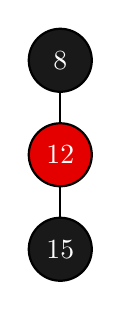
\begin{tikzpicture}[
        scale=0.6,
        red_node/.style={circle, draw, thick, fill=red!90!black, text=white, minimum size=0.8cm},
        black_node/.style={circle, draw, thick, fill=black!90, text=white, minimum size=0.8cm},
        edge/.style={draw, thick, -}
      ]
      % Second tree - middle red
      % Nodes
      \node[black_node] (n8) at (0,0) {8};
      \node[red_node] (n12) at (0,-2) {12};
      \node[black_node] (n15) at (0,-4) {15};
      
      % Edges
      \draw[edge] (n8) -- (n12);
      \draw[edge] (n12) -- (n15);
      \end{tikzpicture}
      \caption{Too many black nodes on right compared to left paths}
      \label{fig:rb-violation2}
    \end{subfigure}
    \hfill 
    \begin{subfigure}[b]{0.24\textwidth}
    \centering
      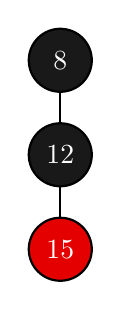
\begin{tikzpicture}[
        scale=0.6,
        red_node/.style={circle, draw, thick, fill=red!90!black, text=white, minimum size=0.8cm},
        black_node/.style={circle, draw, thick, fill=black!90, text=white, minimum size=0.8cm},
        edge/.style={draw, thick, -}
      ]
      % Third tree - bottom red
      % Nodes
      \node[black_node] (n8) at (0,0) {8};
      \node[black_node] (n12) at (0,-2) {12};
      \node[red_node] (n15) at (0,-4) {15};
      
      % Edges
      \draw[edge] (n8) -- (n12);
      \draw[edge] (n12) -- (n15);
      \end{tikzpicture}
      \caption{Too many black nodes on right compared to left paths}
      \label{fig:rb-violation3}
    \end{subfigure}
    \hfill 
    \begin{subfigure}[b]{0.24\textwidth}
    \centering
      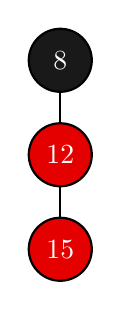
\begin{tikzpicture}[
        scale=0.6,
        red_node/.style={circle, draw, thick, fill=red!90!black, text=white, minimum size=0.8cm},
        black_node/.style={circle, draw, thick, fill=black!90, text=white, minimum size=0.8cm},
        edge/.style={draw, thick, -}
      ]
      % Fourth tree - middle and bottom red
      % Nodes
      \node[black_node] (n8) at (0,0) {8};
      \node[red_node] (n12) at (0,-2) {12};
      \node[red_node] (n15) at (0,-4) {15};
      
      % Edges
      \draw[edge] (n8) -- (n12);
      \draw[edge] (n12) -- (n15);
      \end{tikzpicture}
      \caption{Red node with red child not allowed}
      \label{fig:rb-violation4}
    \end{subfigure}
    \caption{Examples of Red-Black Tree violations.}
    \label{fig:red-black-tree-violations}
  \end{figure}

  This is intentional because red-black tree properties guarantee approximate balance. If we can turn a binary search tree into a red-black tree, then it logically follows that the original BST was approximately balanced. Note that a red black tree does not make searching asymptotically faster in any way; it just takes care of the worst-case. 

\subsection{Tries}


\section{Brute Force Algorithms} 

  So far we have only dealt with algorithms that interact directly with a data structure as an operation. While this is very useful, it's not very fun. Beginning from here, we will consider real-world problems and use data structures more as a \textit{tool} rather than the primary object of study. 

  The first step to building an efficient correct algorithm is to build a correct algorithm, and that is what we focus on here. There are two types of efficiency we have to focus on here. The first is time complexity, which we have done so far. The second refers to the size of the data structures that we use. Obviously we don't want to use a list of size 1000 if a list of size 10 is needed, and so this is referred to as \textit{memory complexity}, which will also be mentioned. 

  Many of these problems will be revisited, either with more efficient solutions or proofs that these brute-force methods are the best that we can do. 

\subsection{Basic Arithmetic}

  In here, we use basic deductions from elementary algebra to give us a starting point at which we analyze fundamental arithmetic algorithms. When we do addition of two numbers, we learn in elementary school to add the least significant digits first and continue on, carrying the $1$ over to the next digit if needed. This is essentially an algorithm. We are also used to doing this in base 10, but we can do it in any base. For reasons that we will see in my computer architecture notes, I will conduct this in base 2. 

  \begin{algo}[Adding Two Integers]
    Given two integers $x, y$ with $n$ bits each, we can add them in the following way. 
    \begin{algorithmic}[1]  
      \Require{$x = x_n \ldots x_1, y = y_n \ldots y_1$}

      \Procedure{Add}{$x$, $y$} 
        \State $z = [0, \ldots, 0]$ of size $n+1$ \Comment{Initialize array to store result.} 
        \State $c = 0$ \Comment{Stores value to carry over}
        \For{$i \gets 1, \ldots n$} 
          \State $z_i \gets x_i + y_i + c$ 
          \If{$z_i > 1$}  
            \State $z_i \gets z_i - 2$ 
            \State $c \gets 1$
          \Else 
            \State $c \gets 0$
          \EndIf  
        \EndFor 
        
        \If{$c > 0$} 
          \State $z[n+1] \gets 1$  
        \EndIf
      \State \Return $z_{n+1} z_n \ldots z_1$
      \EndProcedure
    \end{algorithmic} 

    This gives us a total complexity of $\Theta(n)$, since we are looping over the $n$ bits, plus a constant operation to check for the most significant digit. It also has a memory complexity of $O(n)$.\footnote{Note that we have also used addition in our add function! In here, note that $x_i, y_i, c$ are all either $0$ or $1$, so it will take at most constant time to add all of them. Hence we can treat these addition as $\Theta(1)$. } 
  \end{algo} 

  By the same logic, the time and memory complexity of subtraction are both also $\Theta(n)$ in the number of bits $n$. 

  \begin{algo}[Multiplying Two Integers]
    Given two integers $x, y$ with $n$ bits each, we can multiply them in the following way.
    \begin{algorithmic}[1]  
      \Require{$x = x_n \ldots x_1, y = y_n \ldots y_1$}
      \Procedure{Multiply}{$x$, $y$} 
        \State $z = [0, \ldots, 0]$ of size $2n$ \Comment{Initialize array to store result.} 
        \For{$i \gets 1, \ldots, n$} 
          \If{$y_i = 1$}
            \State $carry \gets 0$
            \For{$j \gets 1, \ldots, n$}
              \State $pos \gets i + j - 1$ \Comment{Position in result}
              \State $sum \gets z_{pos} + x_j + carry$
              \State $z_{pos} \gets sum \bmod 2$
              \State $carry \gets \lfloor sum / 2 \rfloor$
            \EndFor
            \State $z_{i+n} \gets carry$
          \EndIf
        \EndFor
      \State \Return $z_{2n} z_{2n-1} \ldots z_1$
      \EndProcedure
    \end{algorithmic} 
    This algorithm has a time complexity of $O(n^2)$, since for each bit of $y$ we potentially need to perform $n$ additions. The space complexity is $O(n)$ to store the result, which can be up to $2n$ bits long. 
  \end{algo}

  \begin{algo}[Integer Division and Modulus]
    Given two non-negative integers, a dividend $x$ and a divisor $y$, we can compute the quotient $\lfloor x/y \rfloor$ and remainder $r$ such that $x = y \cdot \lfloor x/y \rfloor + r$ and $0 \leq r < y$. This algorithm implements long division in binary, processing the dividend bit by bit from most to least significant. 
    \begin{algorithmic}[1]  
      \Require{$x \geq 0$ with $n$ bits, $y > 0$ with $m$ bits} \Comment{Input: dividend $x$ and divisor $y$}
      \Procedure{Divide}{$x$, $y$} 
        \If{$y = 0$} \Comment{Check for division by zero}
          \State \Return error \Comment{Division by zero is undefined}
        \EndIf
        
        \If{$x < y$} \Comment{Handle case where result is 0}
          \State \Return $(0, x)$ \Comment{Quotient is 0, remainder is $x$}
        \EndIf
        
        \State $quotient \gets 0$ \Comment{Initialize quotient}
        \State $remainder \gets 0$ \Comment{Initialize remainder}
        
        \For{$i \gets n, n-1, \ldots, 1$} \Comment{Process bits from most to least significant}
          \State $remainder \gets 2 \cdot remainder + x_i$ \Comment{Shift remainder left and add next bit}
          
          \If{$remainder \geq y$} \Comment{If remainder is at least the divisor}
            \State $remainder \gets remainder - y$ \Comment{Subtract divisor from remainder}
            \State $quotient \gets quotient \cdot 2 + 1$ \Comment{Set current bit of quotient to 1}
          \Else
            \State $quotient \gets quotient \cdot 2$ \Comment{Set current bit of quotient to 0}
          \EndIf
        \EndFor
        
        \State \Return $(quotient, remainder)$ \Comment{Return both quotient and remainder}
      \EndProcedure
    \end{algorithmic}
    The time complexity is $O(n \cdot m)$, where $n$ is the number of bits in the dividend and $m$ is the number of bits in the divisor. This is because for each of the $n$ bits, we may need to perform a subtraction operation which takes $O(m)$ time. The space complexity is $O(n)$ to store the quotient and $O(m)$ to store the remainder, for a total of $O(n + m)$.
  \end{algo}

  \begin{algo}[Integer Exponentiation]
    Given an integer $x$ with $n$ bits and a non-negative integer exponent $y$, we can compute $x^y$ efficiently using the binary exponentiation method.
    \begin{algorithmic}[1]  
      \Require{$x$ with $n$ bits, $y = y_m \ldots y_1$ with $m$ bits} \Comment{Input: base $x$ and exponent $y$ in binary}
      \Procedure{Exponentiate}{$x$, $y$} 
        \State $result \gets 1$ \Comment{Initialize result to identity element for multiplication}
        \State $base \gets x$ \Comment{Initialize base to the original input value}
        \For{$i \gets 1, \ldots, m$} \Comment{Iterate through each bit of the exponent}
          \If{$y_i = 1$} \Comment{If current bit is set (equals 1)}
            \State $result \gets \text{Multiply}(result, base)$ \Comment{Include current power in the result}
          \EndIf
          \State $base \gets \text{Multiply}(base, base)$ \Comment{Square the base for next iteration (creating $x^{2^i}$)}
        \EndFor
      \State \Return $result$ \Comment{Return the final computed value $x^y$}
      \EndProcedure
    \end{algorithmic} 
    This algorithm has a time complexity of $O(m \cdot n^2)$, where $m$ is the number of bits in the exponent and $n$ is the number of bits in the base. This is because we perform at most $m$ multiplications, and each multiplication (using the standard algorithm) takes $O(n^2)$ time. The space complexity is $O(n \cdot 2^m)$ in the worst case, as the result can grow exponentially with the exponent value.
  \end{algo}

  \begin{algo}[Factorial]
    Given a non-negative integer $n$, we can compute $n!$ as such. 
    \begin{algorithmic}[1]
      \Require{$n \geq 0$} \Comment{Input: non-negative integer $n$}
      \Procedure{Factorial}{$n$}
        \If{$n = 0$ or $n = 1$} \Comment{Handle base cases}
          \State \Return $1$ \Comment{0! = 1! = 1 by definition}
        \EndIf
        
        \State $result \gets 1$ \Comment{Initialize result}
        
        \For{$i \gets 2, 3, \ldots, n$} \Comment{Multiply by each integer from 2 to n}
          \State $result \gets \text{Multiply}(result, i)$ \Comment{Accumulate product}
        \EndFor
        
        \State \Return $result$ \Comment{Return $n!$}
      \EndProcedure
    \end{algorithmic}
    This algorithm implements the direct definition of factorial by iteratively multiplying all integers from 2 to $n$. The time complexity is $O(n \cdot s^2)$, where $n$ is the input value and $s$ is the maximum number of bits needed to represent the intermediate results (which can be up to $O(\log(n!)) = O(n \log n)$ bits). This is because we perform $O(n)$ multiplications, and each multiplication between numbers with $s$ bits takes $O(s^2)$ time using the standard algorithm. The space complexity is $O(s) = O(n \log n)$ to store the result, which grows very rapidly with $n$.
  \end{algo}

\subsection{Lists} 

  \begin{algo}[Max and Min of List]
    Given a list of $n$ elements $A = [a_1, a_2, \ldots, a_n]$, we can find both the maximum and minimum values in the following way.
    \begin{algorithmic}[1]
      \Require{$A = [a_1, a_2, \ldots, a_n]$} \Comment{Input: list of $n$ elements}
      \Procedure{FindMaxAndMin}{$A$}
        \If{length of $A = 0$} \Comment{Handle empty list}
          \State \Return (undefined, undefined)
        \EndIf
        
        \State $max \gets A[1]$ \Comment{Initialize max with first element}
        \State $min \gets A[1]$ \Comment{Initialize min with first element}
        
        \For{$i \gets 2, 3, \ldots, n$} \Comment{Iterate through remaining elements}
          \If{$A[i] > max$} \Comment{Update maximum if needed}
            \State $max \gets A[i]$
          \EndIf
          
          \If{$A[i] < min$} \Comment{Update minimum if needed}
            \State $min \gets A[i]$
          \EndIf
        \EndFor
        
        \State \Return $(max, min)$ \Comment{Return both maximum and minimum}
      \EndProcedure
    \end{algorithmic}
    The time complexity is $\Theta(n)$ since we examine each element exactly once. The space complexity is $O(1)$ as we only use a constant amount of extra space regardless of input size.
  \end{algo}
  
  \begin{algo}[Bubble Sort]
    Given a list of $n$ elements $A = [a_1, a_2, \ldots, a_n]$, we can sort them in ascending order using the bubble sort algorithm.
    \begin{algorithmic}[1]
      \Require{$A = [a_1, a_2, \ldots, a_n]$} \Comment{Input: list of $n$ elements}
      \Procedure{BubbleSort}{$A$}
        \For{$i \gets 1, 2, \ldots, n-1$} \Comment{Outer loop for passes}
          \State $swapped \gets false$ \Comment{Flag to track if any swaps occurred}
          
          \For{$j \gets 1, 2, \ldots, n-i$} \Comment{Inner loop for comparisons}
            \If{$A[j] > A[j+1]$} \Comment{Compare adjacent elements}
              \State Swap $A[j]$ and $A[j+1]$ \Comment{Swap if they are in wrong order}
              \State $swapped \gets true$ \Comment{Set flag to indicate a swap occurred}
            \EndIf
          \EndFor
          
          \If{$swapped = false$} \Comment{If no swaps occurred in this pass}
            \State \textbf{break} \Comment{Array is already sorted, exit early}
          \EndIf
        \EndFor
        
        \State \Return $A$ \Comment{Return sorted list}
      \EndProcedure
    \end{algorithmic}
    The time complexity is $O(n^2)$ in the worst case when the array is in reverse order. In the best case (already sorted), the complexity is $\Theta(n)$ due to the early exit optimization. The space complexity is $O(1)$ as it sorts in-place using only a constant amount of extra space.
  \end{algo}
  
  \begin{algo}[Binary Search]
    Given a sorted list of $n$ elements $A = [a_1, a_2, \ldots, a_n]$ and a target value $x$, we can efficiently search for $x$ in $A$ using binary search.
    \begin{algorithmic}[1]
      \Require{$A = [a_1, a_2, \ldots, a_n]$ (sorted), target value $x$} \Comment{Input: sorted list and target}
      \Procedure{BinarySearch}{$A$, $x$}
        \State $left \gets 1$ \Comment{Initialize left pointer to start of the list}
        \State $right \gets n$ \Comment{Initialize right pointer to end of the list}
        
        \While{$left \leq right$} \Comment{Continue while search space is valid}
          \State $mid \gets \lfloor (left + right) / 2 \rfloor$ \Comment{Calculate middle index}
          
          \If{$A[mid] = x$} \Comment{Target found}
            \State \Return $mid$ \Comment{Return the index where target was found}
          \EndIf
          
          \If{$A[mid] < x$} \Comment{If target is in right half}
            \State $left \gets mid + 1$ \Comment{Update left pointer to search right half}
          \Else \Comment{If target is in left half}
            \State $right \gets mid - 1$ \Comment{Update right pointer to search left half}
          \EndIf
        \EndWhile
        
        \State \Return $-1$ \Comment{Target not found in the list}
      \EndProcedure
    \end{algorithmic}
    The time complexity is $O(\log n)$ since each comparison eliminates approximately half of the remaining elements. The space complexity is $O(1)$ for the iterative implementation shown here, as it uses only a constant amount of extra space regardless of input size.
  \end{algo}

\subsection{Stack, Queues, Heaps}

\subsection{Cryptography} 

  \begin{algo}[GCD of Two Numbers]
    The following is Euclid's algorithm for finding the GCD of two integers. It uses a recursive strategy. 
    \begin{algorithmic}[1]
      \Procedure{GCD}{$a$, $b$} \Comment{Compute greatest common divisor of $a$ and $b$}
        \If{$a = b$} \Comment{Base case: numbers are equal}
          \State \Return $a$
        \ElsIf{$a > b$} \Comment{First recursive case: a is larger}
          \State \Return \Call{GCD}{$a - b$, $b$}
        \Else \Comment{Second recursive case: b is larger}
          \State \Return \Call{GCD}{$a$, $b - a$}
        \EndIf
      \EndProcedure
    \end{algorithmic}
    Example: \Call{GCD}{63, 210} = 21
  \end{algo}

  Note that in order to determine if a number $n$ is prime, we must check all prime number $p < \sqrt{n}$. This gives us the brute force primality testing algorithm. 

  \begin{algo}[Primality Testing]
    Given a positive integer $n > 1$, we can determine whether it is prime as follows.
    \begin{algorithmic}[1]
      \Require{$n > 1$} \Comment{Input: integer to test for primality}
      \Procedure{IsPrime}{$n$}
        \If{$n = 2$ or $n = 3$} \Comment{Handle known small primes}
          \State \Return true
        \EndIf
        
        \If{$n \bmod 2 = 0$ or $n \bmod 3 = 0$} \Comment{Check divisibility by small primes}
          \State \Return false
        \EndIf
        
        \State $i \gets 5$ \Comment{Start checking from 5}
        \While{$i \cdot i \leq n$} \Comment{Check potential divisors up to $\sqrt{n}$}
          \If{$n \bmod i = 0$ or $n \bmod (i + 2) = 0$} \Comment{Check $i$ and $i+2$ (covers all primes > 3)}
            \State \Return false \Comment{Found a divisor, so not prime}
          \EndIf
          \State $i \gets i + 6$ \Comment{Skip to next potential prime pair}
        \EndWhile
        
        \State \Return true \Comment{No divisors found, so number is prime}
      \EndProcedure
    \end{algorithmic}
    This algorithm has a time complexity of $O(\sqrt{n})$, as we check potential divisors up to $\sqrt{n}$. The optimization of checking only numbers of the form $6k \pm 1$ (which covers all primes > 3) reduces the constant factor but does not change the asymptotic complexity. The space complexity is $O(1)$ as we use only a constant amount of extra space.
  \end{algo}

  \begin{algo}[Integer Factorization]
    Given a positive integer $n > 1$, we can find its prime factorization as follows.
    \begin{algorithmic}[1]
      \Require{$n > 1$} \Comment{Input: integer to factorize}
      \Procedure{PrimeFactorize}{$n$}
        \State $factors \gets$ empty list \Comment{Initialize list to store prime factors}
        
        \While{$n \bmod 2 = 0$} \Comment{Extract all factors of 2}
          \State Add $2$ to $factors$
          \State $n \gets n / 2$
        \EndWhile
        
        \While{$n \bmod 3 = 0$} \Comment{Extract all factors of 3}
          \State Add $3$ to $factors$
          \State $n \gets n / 3$
        \EndWhile
        
        \State $i \gets 5$ \Comment{Start checking from 5}
        \While{$i \cdot i \leq n$} \Comment{Check potential prime factors up to $\sqrt{n}$}
          \While{$n \bmod i = 0$} \Comment{Extract all factors of current prime}
            \State Add $i$ to $factors$
            \State $n \gets n / i$
          \EndWhile
          
          \While{$n \bmod (i + 2) = 0$} \Comment{Extract all factors of next potential prime}
            \State Add $(i + 2)$ to $factors$
            \State $n \gets n / (i + 2)$
          \EndWhile
          
          \State $i \gets i + 6$ \Comment{Skip to next potential prime pair}
        \EndWhile
        
        \If{$n > 1$} \Comment{If remaining number is greater than 1, it's prime}
          \State Add $n$ to $factors$
        \EndIf
        
        \State \Return $factors$ \Comment{Return list of prime factors}
      \EndProcedure
    \end{algorithmic}
    This algorithm has a time complexity of $O(\sqrt{n})$ in the worst case, as we check potential prime factors up to $\sqrt{n}$. Similar to the primality test, we use the optimization of checking only numbers of the form $6k \pm 1$ after handling the factors of 2 and 3 explicitly. The space complexity is $O(\log n)$ for storing the prime factors, since a number can have at most $O(\log n)$ prime factors.
  \end{algo}

\subsection{Matrix Operations}

  \begin{algo}[Matrix Multiplication]
    Given two matrices $A$ of size $m \times n$ and $B$ of size $n \times p$, we can compute their product $C = A \times B$ of size $m \times p$ as follows.
    \begin{algorithmic}[1]
      \Require{$A$ is an $m \times n$ matrix, $B$ is an $n \times p$ matrix} \Comment{Input: compatible matrices to multiply}
      \Procedure{MatrixMultiply}{$A$, $B$}
        \State $m \gets$ number of rows in $A$
        \State $n \gets$ number of columns in $A$ \Comment{Also number of rows in $B$}
        \State $p \gets$ number of columns in $B$
        
        \State Initialize matrix $C$ of size $m \times p$ with zeros \Comment{Initialize result matrix}
        
        \For{$i \gets 1, 2, \ldots, m$} \Comment{Iterate through rows of $A$}
          \For{$j \gets 1, 2, \ldots, p$} \Comment{Iterate through columns of $B$}
            \For{$k \gets 1, 2, \ldots, n$} \Comment{Compute dot product of row $i$ of $A$ and column $j$ of $B$}
              \State $C[i][j] \gets C[i][j] + A[i][k] \times B[k][j]$ \Comment{Accumulate sum of products}
            \EndFor
          \EndFor
        \EndFor
        
        \State \Return $C$ \Comment{Return the product matrix}
      \EndProcedure
    \end{algorithmic}
    This algorithm implements the standard matrix multiplication with three nested loops. The time complexity is $O(m n p)$. The space complexity is $O(m p)$ for storing the result matrix. 
  \end{algo}

  \begin{algo}[Matrix Inversion]
    Given a non-singular square matrix $A$ of size $n \times n$, we can compute its inverse $A^{-1}$ using Gaussian elimination with the Gauss-Jordan method.
    \begin{algorithmic}[1]
      \Require{$A$ is an $n \times n$ non-singular matrix} \Comment{Input: invertible square matrix}
      \Procedure{MatrixInverse}{$A$}
        \State $n \gets$ number of rows/columns in $A$
        \State Create augmented matrix $[A|I]$ by appending the identity matrix $I$ of size $n \times n$ to $A$
        
        \For{$i \gets 1, 2, \ldots, n$} \Comment{Forward elimination phase}
          \State Find pivot: maximum absolute value in column $i$ from rows $i$ to $n$
          \If{pivot $= 0$}
            \State \Return error \Comment{Matrix is singular and not invertible}
          \EndIf
          
          \State Swap current row $i$ with pivot row if needed
          
          \State Divide row $i$ by $A[i][i]$ to make the pivot element 1
          
          \For{$j \gets 1, 2, \ldots, n$ where $j \neq i$} \Comment{Eliminate other entries in column $i$}
            \State $factor \gets A[j][i]$
            \For{$k \gets i, i+1, \ldots, 2n$} \Comment{Update augmented matrix row}
              \State $A[j][k] \gets A[j][k] - factor \times A[i][k]$
            \EndFor
          \EndFor
        \EndFor
        
        \State Extract $A^{-1}$ from the right half of the augmented matrix $[I|A^{-1}]$
        \State \Return $A^{-1}$
      \EndProcedure
    \end{algorithmic}
    This algorithm implements the Gauss-Jordan elimination method for matrix inversion. The time complexity is $O(n^3)$ due to the three nested loops, and the space complexity is $O(n^2)$ for storing the augmented matrix. The algorithm transforms the left half of the augmented matrix into the identity matrix, which simultaneously transforms the right half into the inverse matrix.
  \end{algo}
  
  \begin{algo}[Eigendecomposition]
    Given a diagonalizable square matrix $A$ of size $n \times n$, we can compute its eigenvalues and eigenvectors using the power iteration and deflation approach.
    \begin{algorithmic}[1]
      \Require{$A$ is an $n \times n$ diagonalizable matrix} \Comment{Input: diagonalizable square matrix}
      \Procedure{Eigendecomposition}{$A$}
        \State $n \gets$ number of rows/columns in $A$
        \State Initialize empty lists $eigenvalues$ and $eigenvectors$
        \State $A_{current} \gets A$ \Comment{Matrix for deflation process}
        
        \For{$i \gets 1, 2, \ldots, n$}
          \State Initialize random vector $v$ of size $n-i+1$ with unit norm
          \State $prev\_lambda \gets 0$
          \State $lambda \gets 1$
          
          \While{$|lambda - prev\_lambda| > \epsilon$} \Comment{Power iteration until convergence}
            \State $prev\_lambda \gets lambda$
            \State $w \gets A_{current} \times v$ \Comment{Matrix-vector multiplication}
            \State $lambda \gets$ dominant component of $w$
            \State $v \gets w / \|w\|$ \Comment{Normalize vector}
          \EndWhile
          
          \State Add $lambda$ to $eigenvalues$
          \State Add $v$ to $eigenvectors$
          
          \State $A_{current} \gets$ Deflate $A_{current}$ by removing the influence of $\lambda$ and $v$
          \Comment{Deflation: $A_{current} = A_{current} - \lambda \times v \times v^T$}
        \EndFor
        
        \State Construct diagonal matrix $\Lambda$ with $eigenvalues$ on the diagonal
        \State Construct matrix $V$ with $eigenvectors$ as columns
        
        \State \Return $(\Lambda, V)$ \Comment{Return eigenvalue matrix and eigenvector matrix}
      \EndProcedure
    \end{algorithmic}
    This algorithm implements a simplified version of eigendecomposition using power iteration and deflation. The time complexity is $O(k \times n^3)$ where $k$ is the average number of iterations needed for convergence. The space complexity is $O(n^2)$ for storing the matrices. In practice, more sophisticated methods like the QR algorithm are preferred for numerical stability, but the power method illustrates the basic approach.
  \end{algo}

  Given the eigendecomposition is approximately $O(n^3)$, we can also see that computing the singular value decomposition or matrix exponentials are also $O(n^3)$. 

\section{Greedy Algorithms}

  Greedy algorithms are easy to implement and easy to conceptualize, but they are often not correct. So the only interest in them is proving if they are correct. We have done greedy algorithms like Dijkstra and finding MSTs. Every step, greedy algorithms make an irrevocable decision of what to do and cannot undo it. That is, we cannot backtrack. In fact, some algorithms like Kruskal's algorithm for MSTs is precisely a greedy algorithm. 
  
  \begin{example}[Interval Scheduling]
    Let there be 1 classroom and $n$ courses, each with a start and end time $(s_i, e_i)$. We want to find the largest subset of courses that can be scheduled in a day such that they don't overlap. There are two things we want to do. How do we code this up? How do we show that a greedy algorithm will give a correct answer? Two greedy approaches are as follows. 
    \begin{enumerate}
      \item Sort them by the start times, and add them as long as they do not overlap with what you have. This will not work. 
      \item Sort them by the time interval lengths and keep adding them as long as they do not overlap with what you have. This will not work either. 
    \end{enumerate}
    It turns out that if we sort based on finish time, this will work. So why is this correct? Assume that the first $k$ decisions of this greedy algorithm are correct. Then, to find the next interval that we will include, the optimal algorithm must choose one that does not overlap with what we have. This is good since we do the same. The second part is that the next added interval must have the smallest end time $t$ from all viable left intervals. Assume that it was not and that the optimal next interval had end time $s > t$. Then, the next interval must start after $s$, but this also starts after $t$, so we are sacrificing unnecessary extra space. An optimal solution with the endpoint at $s$ can also be constructed with the same interval ending at $t$ without anything to lose. 

    \begin{algorithm}[H]
      \caption{Find Max Classes to Fit into 1 Room}
      \label{alg:class1}
      \begin{algorithmic}
        \Require{classes $C = \{(s_i, e_i)\}_i$ of type \texttt{List[tuple(int, int)]}}
        \Function{Schedule}{\texttt{C}}
          \State $\texttt{res} \gets \texttt{[]}$ 
          \State sort $C$ by increasing end time
          \For{$s, e \in C$} 
            \If{$s < \texttt{res[-1][-1]}$} \Comment{If start overlaps with previous end time}
              \State continue
            \EndIf
            \State add $(s, e)$ to res \Comment{Otherwise add class to final schedule}
          \EndFor
          \State \Return{\texttt{res}}
        \EndFunction
      \end{algorithmic}
    \end{algorithm}
    To get the run time, the sorting takes $O(n \log{n})$ time and iterating is $O(n)$, so a total of $O(n \log{n})$ time. 
  \end{example}

  \begin{example}[Classroom Scheduling]
    A slightly more practical example is that you have $n$ classes and you want to minimize the number of classrooms $m$. For this, you can really use any order. The general idea is 
    \begin{enumerate}
      \item Consider intervals in increasing start time $s_i$. 
      \item If it can be scheduled in an existing classroom, then schedule it there. 
      \item If not, then open a new classroom. 
    \end{enumerate}
    Even then, we can conduct a line search through all the time periods, incrementing the current number of classes if an incoming time is a start time and decrementing if it is an end time. We report the max $\Delta$ over all times. 

    This algorithm is correct since by definition, $\Delta$ is the lower bound for the number of classrooms needed and the greedy algorithm attains it. The greedy algorithm reports $\Delta$ since if it reported $\Delta +1$ classroom, then at some time $t$ it opened the $\Delta+1$th classroom. But this is impossible since this must mean that there are $\Delta + 1$ classrooms concurrently in use, contradicting our assumption that $\Delta$ is the optimal solution. 

    \begin{algorithm}[H]
      \caption{Minimizing Number of Rooms With $n$ Classes (Leetcode 253, Meeting Rooms II)}
      \label{alg:class_schedule}
      \begin{algorithmic}
        \Require{classes $C = \{(s_i, e_i)\}_i$ of type \texttt{List[tuple(int, int)]}}
        \Function{MeetingRooms}{$C$} 
          \State $\texttt{start} \gets$ all start times sorted increasing 
          \State $\texttt{end} \gets$ all end times sorted increasing 
          \State $\texttt{res} \gets 0$ \Comment{Our max classes count} 
          \State $\texttt{count} \gets 0$ \Comment{Our curr. classes count} 
          \State $\texttt{s}, \texttt{e} \gets 0$ \Comment{pointers for \texttt{start}, \texttt{end}} 

          \While{\texttt{s < len(start)}} \Comment{Don't need to check for \texttt{end} since}
            \If{\texttt{start[s] == \texttt{end[e]}}} \Comment{\texttt{start} will always finish faster.}
              \State \texttt{s += 1, e += 1} \Comment{One started and one ended, so don't change}
            \ElsIf{\texttt{start[s] > \texttt{end[e]}}} 
              \State \texttt{e += 1, count -= 1} \Comment{One ended, so decrement \texttt{count}}
            \ElsIf{\texttt{start[s] < \texttt{end[e]}}}
              \State \texttt{s += 1, count += 1} \Comment{One started, so increment \texttt{count}}
              \State \texttt{res = max(res, count)} \Comment{Update res if we got past it}
            \EndIf
          \EndWhile

          \State \Return{res}
        \EndFunction
      \end{algorithmic}
    \end{algorithm}

    The runtime is $O(n \log{n})$, which is to sort. However, you don't even need to sort since you can go through all intervals in any order and place it in an existing classroom or open a new classroom. 
  \end{example}

  The next one isn't as trivial, but requires us to devise a custom sorting method by comparing two sequences with a swap difference. 

  \begin{example}[Quiz Problem]
    Suppose you have $n$ questions with question $i$ having reward $r_i$, but the probability that you get it correct is $p_i$. You keep collecting the reward until you get one question wrong, and the game terminates. What order would you answer the questions in? 

    Suppose we have $q = (10, 5)$ and $r = (0.1, 0.2)$. 
    \begin{enumerate}
      \item If you choose the first and then second, then the expected return is 
        \begin{equation}
          10 \cdot 0.1 + 5 \cdot 0.1 \cdot 0.2 = 1.1 
        \end{equation}

      \item If you choose the second and then first, then the expected return is 
        \begin{equation}
          5 \cdot 0.2 + 10 \cdot 0.1 \cdot 0.2 = 1.2
        \end{equation}
    \end{enumerate}
    Clearly, finding all possibilities is too computationally expensive since it increases exponentially w.r.t. $n$. Intuitively, if I have a question with a high reward, I want to answer it first, but if I have a low probability of getting it correctly, then I can't answer future questions if I get it wrong. So I have to balance these two forces. So we want to sort the score of each question with some function $f(r_i, p_i)$, which is increasing in both $r_i$ and $p_i$. It is not $r_i p_i$, but this is a good start. 
    
    Rather, we can take a different approach. Assume that the tuples were sorted in some order, but this was not the optimal order. Then this indicates that we can swap to adjacent elements and it will get a better order. This is really like bubble sort, and now we need to find out the conditions on which it can be improved.  
    \begin{enumerate}
      \item If we answer $q_1 \rightarrow q_2 \rightarrow q_3 \ldots$, our expected reward is 
        \begin{equation}
          \mathbb{E}[R] = r_1 p_1 + r_2 p_1 p_2 + r_3 p_1 p_2 p_3 
        \end{equation}
      \item If we swap $q_2$ and $q_3$ and answer $q_1 \rightarrow q_3 \rightarrow q_2 \ldots$, then our expected reward is 
        \begin{equation}
          \mathbb{E}[R] = r_1 p_1 + r_3 p_1 p_3 + r_2 p_1 p_2 p_3 
        \end{equation}
      Note that the swap does not affect higher order terms. Doing some algebra, the swap is better iff 
      \begin{equation}
        r_2 p_2 (1 - p_3) < r_3 p_3 (1 - p_2) \implies \frac{r_2 p_2}{1 - p_2} < \frac{r_3 p_3}{1 - p_3}
      \end{equation}
      where the final swap saves computational time since we can compute for a single element rather than comparing pairwise elements. So, we sort it (in descending order!) according to these values to maximize this value. Note that the numerator measures your expected reward, while the denominator measures the probability of you screwing up. 

    \end{enumerate}
  \end{example}

  Not all greedy problems admit to scoring functions however. This was just one example. 

  \begin{example}[Minimizing Max Lateness]
    Suppose there are $n$ jobs that all come in at once at time $0$, with job $j$ having length $p_j$ and deadline $d_j$. We want to schedule the order of jobs on one machine that can handle one job at a time, where you must minimize the maximum lateness, where the lateness of job $i$ is $\max\{f_i - d_i, 0\} = [f_i - d_i]^+$. 

    For example, given jobs $(p, d) = \{(10, 9), (8, 11)\}$, we can run it in two ways. 
    \begin{enumerate}
      \item Running 1 then 2. The first job finishes at $10$ and the second at $18$. The lateness is $10 - 9 = 1$ and $18 - 11 = 7$ respectively, so the maximum lateness is $7$. 
      \item Running 2 then 1. The first job finishes at $8$ and the second at $18$. The lateness is $0$ and $18 - 9 = 9$, so the maximum lateness is $9$.  
    \end{enumerate}
    Therefore, $1 \rightarrow 2$ beats $2 \rightarrow 1$. Clearly, brute forcing this over $N!$ jobs orderings is unfeasible, but there is a greedy approach to this. We can 
    \begin{enumerate}
      \item schedule jobs in increasing order of deadlines. 
      \item try to exchange by taking a sequence, swapping it, and computing the score like we did for previous examples. 
    \end{enumerate}
    Both lead to the same score/principle that we should schedule jobs in increasing order of deadlines. Let's prove this by taking jobs $i$ and $j$, where $d_j \leq d_i$. Then, if we schedule $i \rightarrow j$, then we have 
    \begin{align}
      l_i & = [t + p_i - d_i]^+ \\
      l_j & = [t + p_i + p_j - d_j]^+ 
    \end{align}
    with $l_j$ being the greatest late time. If we did $j \rightarrow i$, then we have 
    \begin{align}
      \hat{l}_j & = [t + p_j - d_j]^+ \\
      \hat{l}_i & = [t + p_i + p_j - d_i]^+ 
    \end{align}
    with $\hat{l}_i$ being the greatest late time. But this is a good sacrifice since we can see that both 
    \begin{equation}
      l_j > \hat{l}_j \text{ and } l_j > \hat{l}_i
    \end{equation}
    meaning that if we swap, then we will decrease the lateness of $j$ at the smaller cost of increasing that of $i$. Therefore, $j \rightarrow i$ is better. Note that even though the end times of the second job will always be the same between the two choices, starting with $j$ will give a later deadline time. So this means that in the optimal solution, we have to place them in this order of deadlines since we can always improve them by swapping. 
  \end{example}

  \begin{example}[Gift Wrapping a Convex Hull]
    Given $n$ points in $\mathbb{R}^2$, we want to find the subset of points on the boundary of its convex hull. We can intuit this by taking the bottom most point and imagine ``wrapping'' a string around the entire region.\footnote{This is called the gift wrapping algorithm.} Here's a basic fact. If we have a point $p_1 = (x_1, y_1)$ and we're looking at $p_2 = (x_2, y_2)$, and then $p_3 = (x_3, y_3)$ shows up, then we can look at the cross product 
    \begin{equation}
      P = (x_2 - x_1) (y_3 - y_1) - (y_2 - y_1)(x_3 - x_1) 
    \end{equation}
    and if $P > 0$, then $p_3$ is counterclockwise from $p_2$. The algorithm is as such. 
    \begin{enumerate}
      \item You choose the bottommost point and label it $p_1$. 
      \item You construct a vector pointing to the right and start turning it counterclockwise until it hits the first point. This can be done by iterating through all of the $n$ points and computing the angle. 
        \begin{equation}
          \tan{ \theta} = \frac{y_i - y_1}{x_i - x_1}
        \end{equation}
      and the points with the smallest such tangent value will be the desired point, which will be $\Theta(n)$. We set this point to be $p_2$ and claim that $p_1, p_2$ is in the convex hull. This is true since all point must lie above the line $p_1 p_2$. Now you do the same thing with $p_2$ starting with a vector facing to the right and rotating it left until it hits the first peg. Once you get to the topmost point, you can start the vector from the right and rotate it counterclockwise, but this is an implementation detail. 

      If your convex hull has $L$ vertices, then this algorithm will have $O(n L)$, which will be $O(n^2)$ worst case but if we sample uniformly, then we have $L \approx \log{n}$ and on average it is $O(n \log{n})$. 
    \end{enumerate}
    A lot of geometric algorithms is output sensitive. 
  \end{example}

  \begin{example}[Convex Hull with Graham Scan]
    In fact, we can take a different approach and get $O(n \log{n})$ time. 
    \begin{enumerate}
      \item You still start with $p_1$ with the minimum y-coordinate and we sort in increasing $\theta_i = \arctan \frac{y_i - y_1}{x_i - x_1}$. 
      \item Then it will walk from $p_i$ to $p_{i+1}$ and check at $p_{i+1}$ if it is on the convex hull or not. 
        \begin{enumerate}
          \item If you turned counterclockwise to go to $p_{i+1}$ then it's good and you're on the convex hull. 
          \item If you turned clockwise it is bad, and $p_i$ is not on the convex hull, so remove $p_i$. However, $p_{i-1}$ could also be clockwise as well, so you must backtrack and keep on removing points until you find a point $p_j$ such that the previous turn is counterclockwise. 
        \end{enumerate}
        Note that this is implemented as a stack. 
    \end{enumerate}
    This can be calculated in $O(1)$ by the previous cross product formula. 
    \begin{figure}[H]
      \centering 
      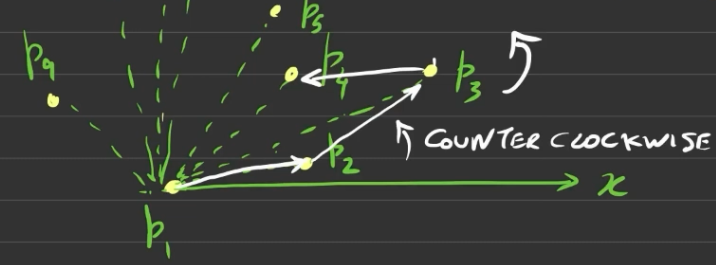
\includegraphics[scale=0.4]{img/graham.png}
      \caption{Overview of the steps mentioned above. } 
      \label{fig:graham}
    \end{figure}
    \begin{algorithm}[H]
      \caption{Finding Convex Hull with Graham Scan}
      \label{alg:graham}
      \begin{algorithmic}
        \Require{$p_1, \ldots, p_n \in \mathbb{R}^2$}
        \Function{Graham}{$\mathbf{p}$} 
          \State s $\gets$ stack()
          \State push $p_1, p_2$ onto s 
          \For{$i = 3, 4, \ldots, n$}
            \State push $p_i$ onto stack 
            \While{top 3 on stack are clockwise}
              \State pop second from top point 
            \EndWhile
          \EndFor 
          \State \Return{s} 
        \EndFunction
      \end{algorithmic}
    \end{algorithm}
    Note that once we have 3 points, the first three in the stack will always be counterclockwise, so we will never need to check if there are enough points in the stack. Even in the beginning, the next point (third) added is guaranteed to be counterclockwise because of ordering. Note that even though we might do a bunch of pushes and pops, the maximum number of pushes we can do is $n$ and pops is $n$, so this is $O(n)$. In fact, the bottleneck is the sorting, which is $O(n \log{n})$, so the total runtime is $O(n \log{n})$. 
  \end{example}

\subsection{Huffman Coding}

  Now, let's talk about \textbf{Huffman encoding}. We already know about the ASCII encoding that encodes characters in $7$ bits, for a total of $2^7$ possibilities. The extended ASCII uses $8$ bits, but all of these things use something called \textbf{fixed-length encoding} which uses a constant number of bits to encode any character. To compress something, we want to use \textbf{variable-length encoding}. 

  To decode something, the mapping from the characters to the bits must be injective, so we can define an inverse over its image. It turns out that if we an encoding for 3 characters, say 
  \[a \mapsto 1, b \mapsto 10, c \mapsto 11\]
  then decoding $1011$ is ambiguous since $1$ is a prefix of the encoding for $c$. Therefore, we do not want one encoding to be the prefix of another. It turns out that we can avoid this conflict by encoding everything as a binary tree and setting all encodings as leaf nodes. 
  \begin{center}
      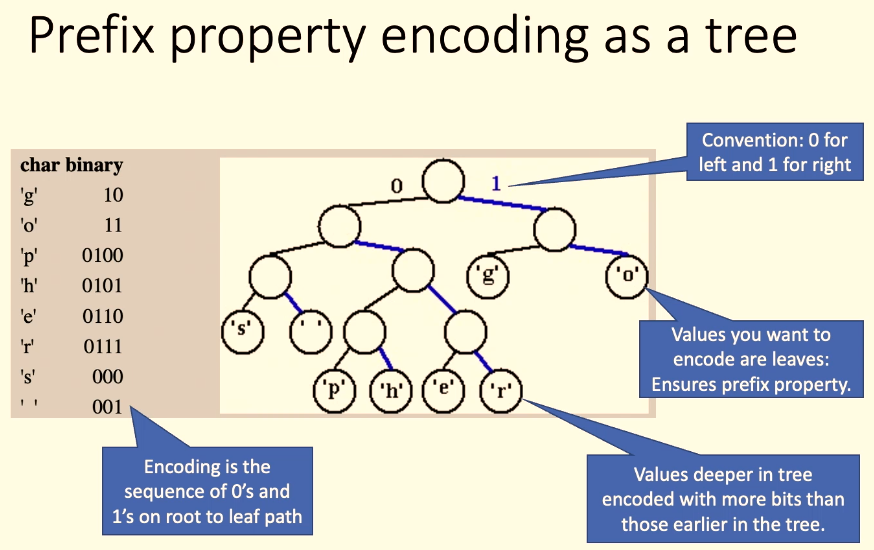
\includegraphics[scale=0.5]{img/Tree_Encoding.png}
  \end{center}
  This makes sense since an encoding will be a prefix of another if and only if it is a parent of another. Furthermore, a greater depth of a character in the tree corresponds to a longer encoding. So, Huffman encoding tries to convert shorter characters to longer leaves and less recurrent characters into longer encodings. To decode a string of bits using a tree, we read the bit at a time to traverse left or right edge. When we reach a leaf, we decode the character and restart at root. 

  Now, we describe the greedy algorithm for building an optimal variable length encoding tree. 
  \begin{enumerate}
      \item We take the document and compute the frequencies of all characters that we want to encode. We want to less frequent characters to be lower on the tree, and so we will build the tree up from the leaves. 
      \item We iteratively choose the lowest weight nodes to connect up to a new node with weight = sum of children. 
  \end{enumerate}
  We implement this using a priority queue. 

  \begin{example}
    Let us go do an example of where we have the characters and frequencies 
    \begin{equation}
      a \mapsto 30, \; b \mapsto 20, \; c \mapsto 10, \; d \mapsto 15, \; e \mapsto 40
    \end{equation}

    \begin{figure}[H]
      \centering
      \begin{subfigure}[b]{0.48\textwidth}
      \centering
        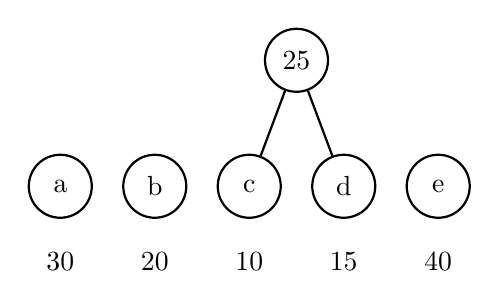
\begin{tikzpicture}[
            scale=0.8,
            node/.style={circle, draw, thick, minimum size=0.8cm},
            edge/.style={-,thick}
        ]
        % Vertices a through e at the bottom
        \node[node] (a) at (0,0) {a};
        \node[node] (b) at (1.5,0) {b};
        \node[node] (c) at (3,0) {c};
        \node[node] (d) at (4.5,0) {d};
        \node[node] (e) at (6,0) {e};
        % The vertex 25 at the top, positioned between c and d horizontally
        \node[node] (v5) at (3.75,2) {25};
        % Connect 25 to c and d
        \draw[edge] (v5) -- (c);
        \draw[edge] (v5) -- (d);
        % Add labels below the bottom vertices with increased spacing
        \node at (0,-1.2) {30};
        \node at (1.5,-1.2) {20};
        \node at (3,-1.2) {10};
        \node at (4.5,-1.2) {15};
        \node at (6,-1.2) {40};
        \end{tikzpicture}
        \caption{We write out them as leaf nodes with the values $30, 20, 10, 15, 40$. We take the smallest of the frequencies and sum them up: $10 + 15 = 25$.}
        \label{fig:step1}
      \end{subfigure}
      \hfill 
      \begin{subfigure}[b]{0.48\textwidth}
      \centering
        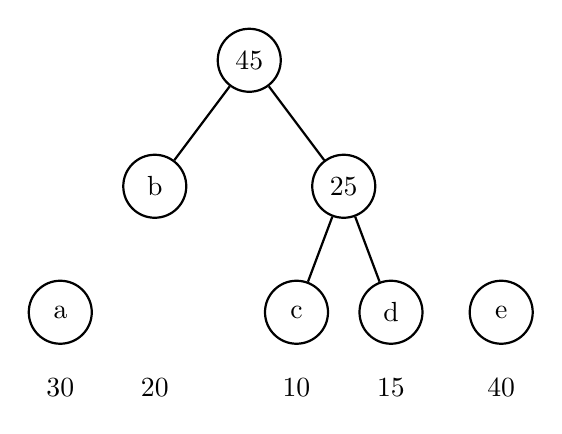
\begin{tikzpicture}[
            scale=0.8,
            node/.style={circle, draw, thick, minimum size=0.8cm},
            edge/.style={-,thick}
        ]
        % Top node (45)
        \node[node] (root) at (3,4) {45};
        % Second level nodes
        \node[node] (b) at (1.5,2) {b};
        \node[node] (v25) at (4.5,2) {25};
        % Bottom level connected nodes
        \node[node] (c) at (3.75,0) {c};
        \node[node] (d) at (5.25,0) {d};
        % Isolated nodes
        \node[node] (a) at (0,0) {a};
        \node[node] (e) at (7,0) {e};
        % Connections
        \draw[edge] (root) -- (b);
        \draw[edge] (root) -- (v25);
        \draw[edge] (v25) -- (c);
        \draw[edge] (v25) -- (d);
        % Add labels below the bottom vertices with good spacing
        \node at (0,-1.2) {30};
        \node at (1.5,-1.2) {20};
        \node at (3.75,-1.2) {10};
        \node at (5.25,-1.2) {15};
        \node at (7,-1.2) {40};
        \end{tikzpicture}
        \caption{We have the values $30, 20, 25, 40$. We sum the smallest two frequencies: $20 + 25 = 45$.}
        \label{fig:step2}
      \end{subfigure}
      
      \begin{subfigure}[b]{0.48\textwidth}
      \centering
        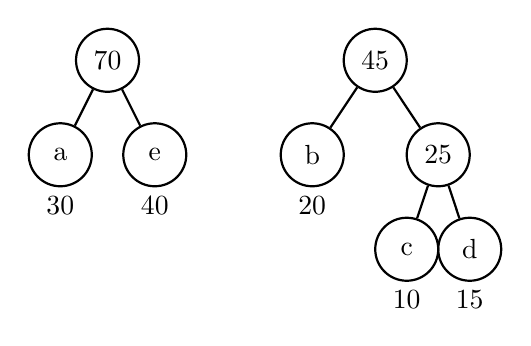
\begin{tikzpicture}[
            scale=0.8,
            node/.style={circle, draw, thick, minimum size=0.8cm}, % Smaller nodes
            edge/.style={-,thick}
        ]
        % Left tree - with reduced distances
        % Top node (70)
        \node[node] (left_root) at (-1.5,3) {70};
        % Bottom level for left tree
        \node[node] (a) at (-2.25,1.5) {a};
        \node[node] (e) at (-0.75,1.5) {e};
        % Connections for left tree
        \draw[edge] (left_root) -- (a);
        \draw[edge] (left_root) -- (e);
        % Add labels below the left tree nodes
        \node at (-2.25,0.7) {30};
        \node at (-0.75,0.7) {40};
        
        % Right tree - with reduced distances
        % Top node (45)
        \node[node] (right_root) at (2.75,3) {45};
        % Second level nodes for right tree
        \node[node] (b) at (1.75,1.5) {b};
        \node[node] (v25) at (3.75,1.5) {25};
        % Bottom level for right tree
        \node[node] (c) at (3.25,0) {c};
        \node[node] (d) at (4.25,0) {d};
        % Connections for right tree
        \draw[edge] (right_root) -- (b);
        \draw[edge] (right_root) -- (v25);
        \draw[edge] (v25) -- (c);
        \draw[edge] (v25) -- (d);
        % Add labels below the right tree nodes
        \node at (1.75,0.7) {20};
        \node at (3.25,-0.8) {10};
        \node at (4.25,-0.8) {15};
        \end{tikzpicture}
        \caption{We have the values $30, 45, 40$. We sum the smallest two frequencies: $30 + 40 = 70$.}
        \label{fig:step3}
      \end{subfigure}
      \hfill 
      \begin{subfigure}[b]{0.48\textwidth}
      \centering
        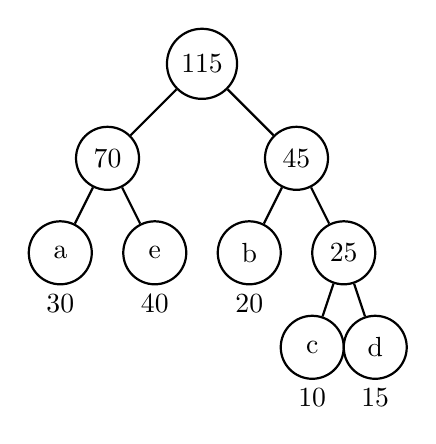
\begin{tikzpicture}[
            scale=0.8,
            node/.style={circle, draw, thick, minimum size=0.8cm}, % Smaller nodes
            edge/.style={-,thick}
        ]
        % More compact layout with reduced distances
        % Top node (115)
        \node[node] (root) at (2.25,4.5) {115};
        % Second level nodes
        \node[node] (v70) at (0.75,3) {70};
        \node[node] (v45) at (3.75,3) {45};
        % Connect top to second level
        \draw[edge] (root) -- (v70);
        \draw[edge] (root) -- (v45);
        % Third level nodes for left branch
        \node[node] (a) at (0,1.5) {a};
        \node[node] (e) at (1.5,1.5) {e};
        % Connect v70 to its children
        \draw[edge] (v70) -- (a);
        \draw[edge] (v70) -- (e);
        % Third level nodes for right branch
        \node[node] (b) at (3,1.5) {b};
        \node[node] (v25) at (4.5,1.5) {25};
        % Connect v45 to its children
        \draw[edge] (v45) -- (b);
        \draw[edge] (v45) -- (v25);
        % Fourth level nodes
        \node[node] (c) at (4,0) {c};
        \node[node] (d) at (5,0) {d};
        % Connect v25 to its children
        \draw[edge] (v25) -- (c);
        \draw[edge] (v25) -- (d);
        % Add labels below the bottom vertices
        \node at (0,0.7) {30};
        \node at (1.5,0.7) {40};
        \node at (3,0.7) {20};
        \node at (4,-0.8) {10};
        \node at (5,-0.8) {15};
        \end{tikzpicture}
        \caption{We have the values $70, 45$. We sum them up to get the complete tree.}
        \label{fig:step4}
      \end{subfigure}
      \caption{Building a Huffman encoding tree step by step}
      \label{fig:huffman-construction}
    \end{figure}
  \end{example}

  \begin{theorem}[Number of Nodes in Huffman Tree]
    If we have a document of $N$ total characters and $M$ unique characters, the number of nodes in the Huffman tree, in complexity notation, is 
    \begin{equation}
      O(M)
    \end{equation}
    Clearly, this has nothing to do with $N$. Note that we have $M$ leaf nodes, and in each iteration, we connect 2 nodes up to a parent. Therefore, the number of nodes to connect up decreases by 1 per iteration, and we create a new node per iteration. Since there are $M - 1$ iterations, we add one node, so there will be $M + M - 1 = O(n)$ nodes in the binary tree. 
  \end{theorem}


\section{Divide and Conquer} 

  \begin{definition}[Divide and Conquer Algorithms]
    The general idea is two steps: 
    \begin{enumerate}
      \item Divide an input into smaller instances of the same problem. The simplest form is merge sort. 
      \item Conquer/solve these smaller instances, which takes less time. 
      \item Merge/Combine the smaller solutions into the original, bigger solution. 
    \end{enumerate}
    This is usually recursive, but does not need to be. 
  \end{definition}

  It has its applications in the most elementary operations, in sorting and multiplication. To prove correctness, we use induction by proving the correctness of the base case and then the inductive step to show that there is an invariant. 

\subsection{Recursive Algorithms and Recurrence Relation}

  I assume that the reader is familiar with recursive algorithms. Now to evaluate the runtime of a recursive algorithm, one must implicitly solve for the runtime of its recursive calls, and we can visualize it. 

  \begin{figure}[H]
    \centering 
    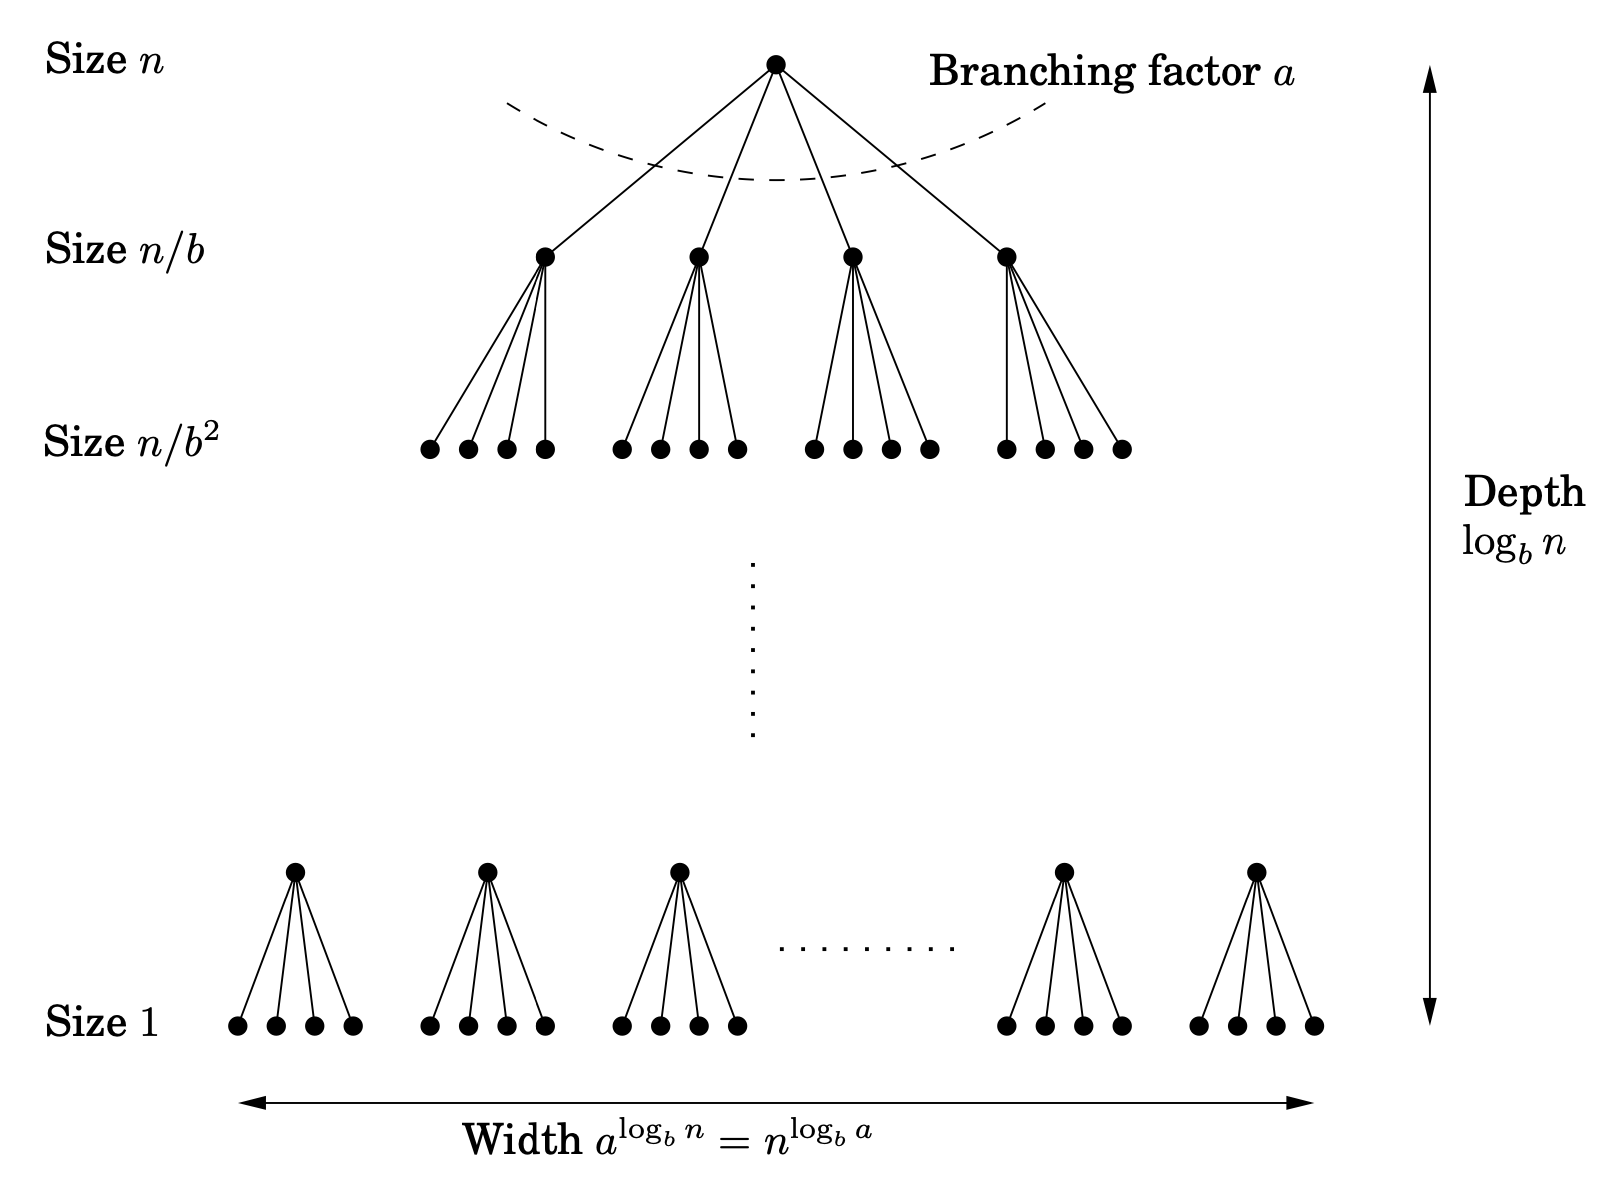
\includegraphics[scale=0.4]{img/branching.png}
    \caption{} 
    \label{fig:branching}
  \end{figure}

  An important theorem for divide-and-conquer algorithms is 

  \begin{theorem}[Master Theorem]
    Given a recurrence relation of form 
    \begin{equation}
      T(N) = a T(N/b) + O(N^c)
    \end{equation}
    then the following holds 
    \begin{align}
      a > b^c & \implies T(N) = O(N^{\log_b a}) \\
      a = b^c & \implies T(N) = O(N^c \log{N}) \\
      a < b^c & \implies T(N) = O(N^c) 
    \end{align}
  \end{theorem}
  \begin{proof}
    To intuit this, see that if $a > b^c$, then there arises a lot of subproblems, so our complexity is greater. If $a < b^c$, then we have few subproblems and can get a better runtime. If $a = b^c$, we get somewhere in between. To actually solve this, we can just unravel the recurrence to get the infinite series 
    \begin{align}
      T(N) & = a T(N/b) + O(N^c) \\
           & = a^2 T(N/b^2) +  N^c \bigg( \frac{a}{b^c} + 1 \bigg) \\
           & =  N^c \bigg( 1 + \frac{a}{b^c} + \frac{a^2}{b^{2c}} + \ldots \bigg)
    \end{align}
    So, if $a < b^c$, then even as $N \rightarrow \infty$, the sum is finite, so it is of order $O(N^c)$. If $a = b^c$, then the series is just $1 + \ldots + 1$, which scales on the order of $O(\log_2 {N})$. If $> 1$, then we have to calculate the last term, which contributes to our runtime and overpowers $c$.  
    
    Therefore, if $a$ is large, our algorithm will have an exponential number of subproblems and will be bottlenecked by the. 
  \end{proof}

\subsection{Merge Sort and Counting Inversions}

  \begin{algo}[Merge Sort]
    Merge sort is the first instance. 
    \begin{algorithm}[H]
      \caption{Merge Sort}
      \label{alg:merge_sort}
      \begin{algorithmic}
        \Require{Array \texttt{nums}}
        \Function{MergeSort}{\texttt{nums}}
          \State \texttt{n = len(nums)}

          \If{\texttt{n < 2}} \Comment{base case}
            \State \Return{nums}
          \EndIf
          \State \texttt{mid = n // 2} 
          \State \texttt{left\_sorted = MergeSort(nums[:mid])} \Comment{Divide into left half}
          \State \texttt{right\_sorted = MergeSort(nums[mid:])} \Comment{Divide into right half}

          \State \texttt{res = [0] * n} 
          \State \texttt{i = j = k = 0} 
          \While{\texttt{k < n}} \Comment{Merge the sorted subarrays}
            \If{\texttt{j == len(right\_sorted) or left\_sorted[i] < right\_sorted[j]}}
              \State \texttt{res[k] = left\_sorted[i]} \Comment{We should add the next element from left array}
              \State \texttt{i += 1} \Comment{if it is smaller or if right array is filled already}
            \Else 
              \State \texttt{res[k] = right\_sorted[j]}
              \State \texttt{j += 1}
            \EndIf 
            \State \texttt{k += 1}
          \EndWhile

          \State \Return{\texttt{res}}
        \EndFunction
      \end{algorithmic}
    \end{algorithm}
    The recurrence relation for the runtime is as follows. Let $T(n)$ represent the worst-case runtime of \texttt{MergeSort} of size $n$. Then, we have 
    \begin{equation}
      T(n) = 2 \cdot T(n/2) + O(n)
    \end{equation}
    Consisting of two recursive calls with input size $n/2$ and then the merge step which is $O(n)$. But if we take a look at this, we have 
    \begin{align}
      T(n) & = 2 \cdot T(n/2) + O(n) \\
           & = 2 \cdot \big( 2 \cdot T(n/4) + O(n/2)) + O(n) \\
           & = 4 \cdot T(n/4) + O(n) + O(n) 
    \end{align}
    and the number of times $O(n)$ is added up is $\log{n}$, meaning that this recurrence relation turns into $O(n \log{n})$. 
  \end{algo}

  \begin{definition}[Inversions]
    Given two lists of ranked items, say 
    \begin{align}
      \text{Alice}: & a > b > c > d > e \\
      \text{Bob}: & b > d > a > e > c
    \end{align}
    We want to measure the dissimilarity between two rankings by counting the number of \textit{inversions}, which are pairs of items for which open persons orders the opposite of the other (e.g. $a, b$ for above).\footnote{Also known as Kendall-Tau distance in statistics.} So how many inversions are there? We can do this in $\Theta(n^2)$ by explicitly looking at all $n$ pairs. Without loss of generality, we can assume that the first list is sorted simply by bijectively relabeling these elements for both lists. Therefore, the set of inversions is defined to be 
    \begin{equation}
      \{(i, j) \text{ s.t. } i < j \text{ and } \texttt{A[i] > A[j]}\}
    \end{equation}
  \end{definition}

  \begin{algo}[Counting Inversions]
    The idea is very similar. By assuming that the first list is sorted, we can simply count the number of inversions in a single list $A$.  
    \begin{lstlisting}
      A = 5 6 1 3 4 8 2 7
    \end{lstlisting}
    \begin{enumerate}
      \item In the divide step, we count all inversions in $A_l, A_r$, which are the left and right sides of $A$, \textit{and} we sort $A_l, A_r$ to add additional structure.  
        \begin{lstlisting}
          1 3 5 6 | 2 4 7 8
        \end{lstlisting}
      \item In the conquer step, we merge them linearly but every time we add an element from $A_r$ into our result, this reveals that there are $k$ additional inversions added where $k$ is the number of elements left in $A_l$ to add.  
    \end{enumerate}
    \begin{algorithm}[H]
      \caption{Counting Inversions}
      \label{alg:inversions}
      \begin{algorithmic}
        \Require{Array \texttt{nums}}
        \Function{Inversions}{\texttt{nums}}
          \State \texttt{n = len(nums)}

          \If{\texttt{n < 2}} \Comment{base case}
            \State \Return{nums}
          \EndIf
          \State \texttt{mid = n // 2} 
          \State \texttt{left\_sorted, left\_invs = Inversions(nums[:mid])} \Comment{Divide into left half}
          \State \texttt{right\_sorted, right\_invs = Inversions(nums[mid:])} \Comment{Divide into right half}

          \State \texttt{res = [0] * n} 
          \State \texttt{i = j = k = 0} \Comment{left, right, and combined index}
          \State \texttt{inv = 0} \Comment{number of inversions}
          \While{\texttt{k < n}} \Comment{Merge the sorted subarrays}
            \If{\texttt{j == len(right\_sorted) or left\_sorted[i] < right\_sorted[j]}}
              \State \texttt{res[k] = left\_sorted[i]} \Comment{We should add the next element from left array}
              \State \texttt{invs += len(left\_sorted - i)} \Comment{Increment inversions by \# of elems in left array}
              \State \texttt{i += 1} \Comment{if it is smaller or if right array is filled already}
            \Else 
              \State \texttt{res[k] = right\_sorted[j]}
              \State \texttt{j += 1}
            \EndIf 
            \State \texttt{k += 1}
          \EndWhile

          \State \Return{\texttt{res, inv + left\_invs + right\_invs}}
        \EndFunction
      \end{algorithmic}
    \end{algorithm}
    The recursion relation is still 
    \begin{equation}
      T(n) = 2 \cdot T(n/2) + O(1) + O(n) \implies O(n \log{n})
    \end{equation}
  \end{algo}

\subsection{Selection and Quick Sort} 

  The next problem is a generalization of finding the median of an array, which we present can be done in $O(n)$ time \textit{on average}. It turns out that that this idea of choosing a pivot and then dividing and conquering happens often in general selection and sort algorithms.    

  \begin{algo}[Select kth Largest Element from Unsorted Array]

    \begin{algorithm}[H]
      \caption{Find Kth Largest Element}
      \label{alg:kth_largest}
      \begin{algorithmic}
        \Require{Array of numbers nums, integer k where 1 <= k <= length(nums)}
        \State
        \Function{FindKthLargest}{nums, k}
            \If{length(nums) = 1} \Comment{Base case: if array has only one element}
                \State \Return nums[0]
            \EndIf
            
            \State pivot $\gets$ $\lfloor$length(nums)/2$\rfloor$ \Comment{Select middle element as pivot}
            \State left $\gets$ [ ] \Comment{Unsorted array for elements smaller than pivot}
            \State right $\gets$ [ ] \Comment{Unsorted array for elements larger than pivot}
            \State n\_pivots $\gets$ 0 \Comment{Count of elements equal to pivot}
            
            \For{each n in nums} \Comment{Start filling in the arrays}
                \If{n = nums[pivot]}
                    \State n\_pivots $\gets$ n\_pivots + 1
                \ElsIf{n $\leq$ nums[pivot]}
                    \State left.append(n)
                \Else
                    \State right.append(n)
                \EndIf
            \EndFor
            
            \If{length(right) $\leq$ k - 1 \textbf{and} length(left) $\leq$ length(nums) - k}
              \State \Return nums[pivot] \Comment{Found the $k$th element which was in the middle in n\_pivots}
            \ElsIf{length(right) $\geq$ k}
              \State \Return \Call{FindKthLargest}{right, k} \Comment{Largest is in the array of bigger numbers.}
            \Else
              \State \Return \Call{FindKthLargest}{left, k - length(right) - n\_pivots} \Comment{Largest is in the array of smaller numbers.}
            \EndIf
        \EndFunction
      \end{algorithmic}
    \end{algorithm}
  \end{algo}

  \begin{algo}[Quick Sort]
    
    \begin{algorithm}[H]
      \caption{Quicksort Algorithm}
      \label{alg:quicksort}
      \begin{algorithmic}
        \Require{Array A of comparable elements}
        \State
        \Function{Quicksort}{A, low, high}
            \If{low < high}
                \State p $\gets$ \Call{Partition}{A, low, high} \Comment{Get pivot position}
                \State \Call{Quicksort}{A, low, p - 1} \Comment{Sort left subarray}
                \State \Call{Quicksort}{A, p + 1, high} \Comment{Sort right subarray}
            \EndIf
        \EndFunction
        \State
        \Function{Partition}{A, low, high}
            \State pivot $\gets$ A[high] \Comment{Choose rightmost element as pivot}
            \State i $\gets$ low - 1 \Comment{Index of smaller element}
            
            \For{j $\gets$ low to high - 1} \Comment{Scan through array}
                \If{A[j] $\leq$ pivot}
                    \State i $\gets$ i + 1 \Comment{Increment index of smaller element}
                    \State swap A[i] and A[j] \Comment{Swap current element with pivot}
                \EndIf
            \EndFor
            \State swap A[i + 1] and A[high] \Comment{Put pivot in its correct position}
            \Return i + 1 \Comment{Return pivot's final position}
        \EndFunction
      \end{algorithmic}
    \end{algorithm}
  \end{algo}

\subsection{Closest Pair of Points} 

  The next problem simply takes a series of points and calculates the closest pair of points. This can be done trivially in $O(N^2)$ by taking all combinations, but with clever divide and conquer, we can reduce this down. The idea is that we want to divide them into a left and a right side, which we can sort in $O(N \log{N})$ and find the median in $O(1)$. This now reduces to computing the closest pair of points in each $N/2$ half. If we can find the closest pair in each half, then we must compare it to all pairs of points across the halves, meaning that we must do $(N/2)^2$ comparisons again, leading to 
  \begin{equation}
    T(N) = 2 T(N/2) + O(N^2)
  \end{equation}
  which isn't any better than $O(N^2)$. But imagine that we found that the smallest distance of the left and right were $\delta_1, \delta_2$, then for each point in the left side, we don't have to check all $N/2$ points on the right. 

  \begin{figure}[H]
    \centering 
    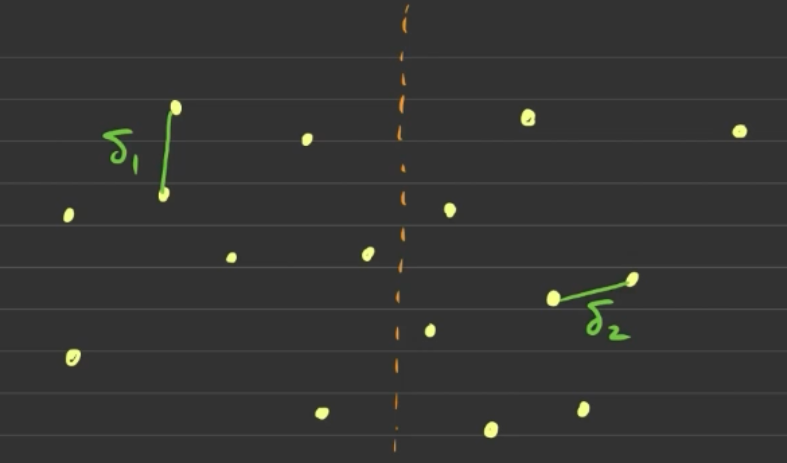
\includegraphics[scale=0.4]{img/closest_point.png}
    \caption{} 
    \label{fig:closest_point}
  \end{figure}

  We just have to check those with distance at most $\delta = \min\{\delta_1, \delta_2\}$ from each point. Furthermore, we can discard all points that are too far away from the boundary. However, all $N$ points could like in the relevant space, leading to $O(N^2)$ computations of distance. 

  \begin{figure}[H]
    \centering 
    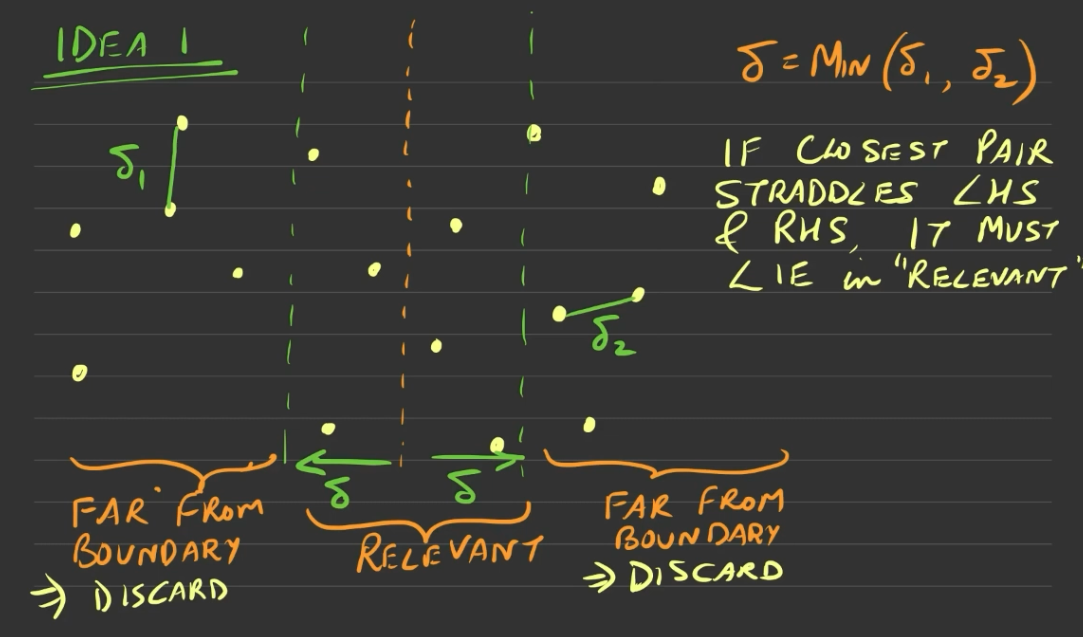
\includegraphics[scale=0.4]{img/cp2.png}
    \caption{} 
    \label{fig:closest_point2}
  \end{figure}

  Therefore, we want to incorporate vertical distances and tile our relevant space into square of side length $\delta/2$.  

  \begin{figure}[H]
    \centering 
    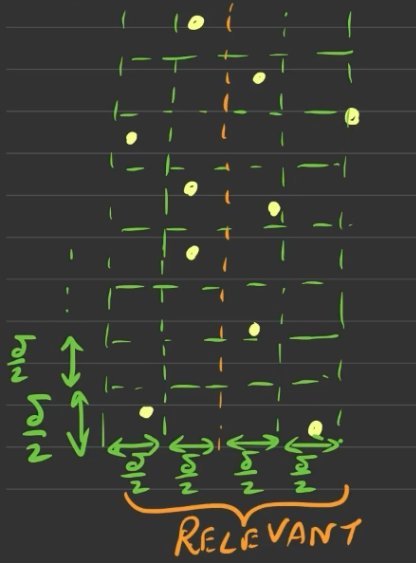
\includegraphics[scale=0.4]{img/cp3.png}
    \caption{} 
    \label{fig:closest_point3}
  \end{figure}

  We claim that each square has at most 1 point, since if there were two, then their distance would be less than $\delta / \sqrt{2}$, which contradicts the distance between the two points being greater than $\delta$. Therefore given a point, we only need to check a bounded constant. 

  \begin{figure}[H]
    \centering 
    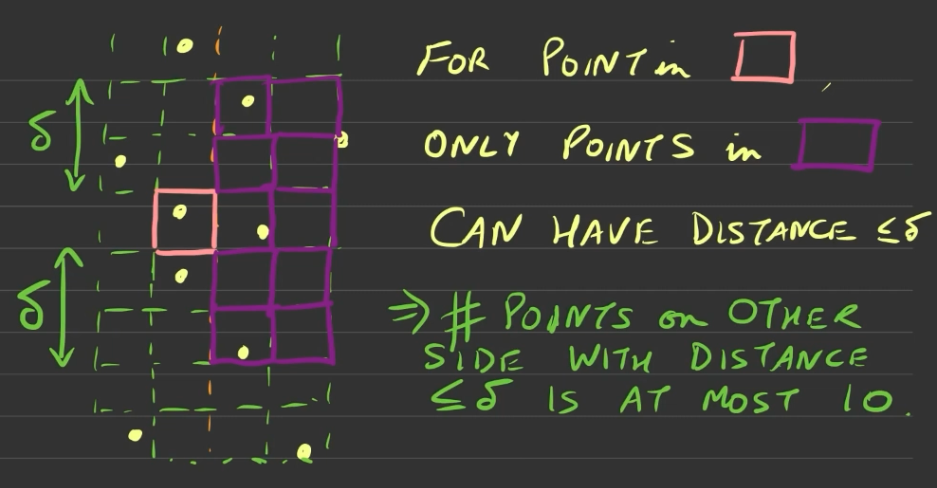
\includegraphics[scale=0.4]{img/cp4.png}
    \caption{The number of points on the other side with distance $\leq \delta$ is at most $10$. If we are more careful, we can reduce the number down to $7$. } 
    \label{fig:closest_point4}
  \end{figure}

  It turns out that we just need to compute $5N = (N/2) \cdot 10$ distances at most, and now our question reduces to how do we find these 5 points? Well we can first sort the points on the left and right by their y-coordinates, so we can just take a sliding window that encapsulates these points on the right for every on the left. The pointers of the sliding window should point to a point where the y-coordinate is at most $\delta$ away, and this can be done in constant time. Therefore, our recurrence relation is  

  \begin{equation}
    T(N) = 2 T(N/2) + O(N \log{N}) \implies T(N) = O(N \log^2 {N})
  \end{equation}
  
  This sorting along the y-coordinates is a bottleneck, but we can just shove this into the recursion step by telling the left and right to not just return the $\delta_1, \delta_2$, but also the points sorted in the y-coordinate. Then at the end of the merge, we also merge the lists $L, R$ so that $S = L \cup R$ is sorted on $y$, which also takes $O(N)$ and doesn't add extra runtime on the merge step. This reduces the runtime to $O(N \log{N})$. 

  \begin{algo}[Closest Pair of Points]
    The next problem simply takes a series of points and calculates the closest pair of points. This can be done trivially in $O(N^2)$ by taking all combinations, but with clever divide and conquer, we can reduce this down. 
    \begin{algorithm}[H]
      \caption{Closest Pair of Points}
      \label{alg:closest_pair}
      \begin{algorithmic}
        \Require{$N$ points $\{(x_i, y_i)\}$.}
        \State 
        \Function{ClosestPair}{P} 
          \State Sort points by x-coordinate. \Comment{Bottleneck of $O(N \log{N})$}
          \If{len(P) = 2} 
            \State \Return $d(p_1, p_2)$, sorted $P$ by y-coord
          \EndIf

          \State $\delta_1, L \gets$ ClosestPair($P_L$)
          \State $\delta_2, R \gets$ ClosestPair($P_R$)
          \State $\delta = \min\{\delta_1, \delta_2\}$ 
          \State min $\gets \delta$
          \For{$l \in L$ s.t. distance to boundary $\leq \delta$} \Comment{$O(N)$ iterations}
            \State $W_l \gets \delta$-window of points in $R$ around $l$. \Comment{Can be done in $O(1)$ using sliding window.}
            \For{$r \in W_l$} \Comment{This is bounded by $O(10)$}
              \If{$d(p, l) < \delta$} 
                \State min $\gets d(p, l)$
              \EndIf
            \EndFor
          \EndFor

          \State merge $L$ and $R$ into sorted $S$ \Comment{O(N)} 

          \State \Return{min, S}
        \EndFunction
      \end{algorithmic}
    \end{algorithm}
  \end{algo}

\subsection{Multiplication}

  \subsubsection{Karatsuba Algorithm}


  \subsubsection{Strassen Algorithm}

    We can solve matrix multiplication of two $N \times N$ matrices in a slightly more clever way than $O(N^3)$. Note that we can take the $2 \times 2$ block form of matrices $A, B$ and multiply them to get $C = AB$, where 
    \begin{align}
      C_{11} & = A_{11} B_{11} \cdot A_{12} B_{21} \\ 
      C_{12} & = A_{11} B_{12} \cdot A_{12} B_{22} \\ 
      C_{21} & = A_{21} B_{11} \cdot A_{22} B_{21} \\ 
      C_{22} & = A_{21} B_{12} \cdot A_{22} B_{22} 
    \end{align}

    This requires us to compute a total of $8$ $N/2 \times N/2$ multiplications and 4 additions, each of which is $O(N^2)$. Therefore, our recurrence relation is 
    \begin{equation}
      T(N) = 8 T(N/2) + O(N^2)
    \end{equation}

    Using the master theorem, we find that $a = 8 > 2^2 = b^c$, so our runtime is $O(N^{\log_{b} a}) = O(N^3)$, which brings us right back to where we started. The problem with this is that $a = 8$, which is large. If we could get $a = 7$, then this would be an improvement. We want to reduce this number of multiplications, and we can do this using the Strassen algorithm, which uses the following values.  
    \begin{align*}
      P_1 &= (a_{11} + a_{22}) (b_{11} + b_{22}) \\
      P_2 &= (a_{21} + a_{22}) b_{11} \\
      P_3 &= a_{11} (b_{12} - b_{22}) \\
      P_4 &= a_{22} (b_{21} - b_{11} \\
      P_5 &= (a_{11} + a_{12}) b_{22} \\
      P_6 &= (a_{21} - a_{11}) (b_{11} + b_{12}) \\
      P_7 &= (a_{12} - a_{22}) (b_{21} + b_{22}) 
    \end{align*}
    Then, we claim that we the entries of $C$ are 
    \begin{align*}
        c_{11} &= P_1 + P_4 - P_5 + P_7 \\
        c_{12} &= P_3 + P_5 \\
        c_{21} &= P_2 + P_4 \\
        c_{22} &= P_1 + P_3 - P_2 + P_6
    \end{align*}
    So we have reduced 8, 4 mult/add to 7, 18 mult/add. Addition is cheap and the number of additions is bounded, so now we have decreased $a$ to $7$.\footnote{We can reduce it even further, down to $2.37$. Whether $O(N^2)$ is possible is an open problem. } We can then solve the new recurrence relation 
    \begin{equation}
      T(N) = 7 T(N/2) + O(N^2) \implies O(N^{\log_2 7}) \approx O(N^{2.81})
    \end{equation}

\subsection{Polynomial Multiplication with Fast Fourier Transform}

  Given as inputs $2$ degree $N$ polynomials, 
  \begin{align}
    A(x) & = a_0 + a_1x + a_2x^2 + \ldots + a_{n-1}x^{n-1} \\
    B(x) & = b_0 + b_1x + b_2x^2 + \ldots + b_{n-1}x^{n-1} 
  \end{align}
  we want to multiply them to $C(x) = A (x) B(x)$ defined 
  \begin{equation}
    C(x) = c_0 + c_1x + \cdots + c_{2n-2}x^{2n-2} 
  \end{equation}
  Clearly, we must multiply every coefficient in $A$ with $B$, which takes $O(N^2)$ time. It is also called the convolution operation. 
  \begin{align*}
    &\text{Convolution of } (a_0, a_1, \ldots, a_{n-1}) \text{ and } (b_0, b_1, \ldots, b_{n-1}) \\[1em]
    &c_0 = a_0 b_0 \\
    &c_1 = a_0 b_1 + a_1 b_0 \\
    &c_2 = a_0 b_2 + a_1 b_1 + a_2 b_0 \\
    &c_3 = a_0 b_3 + a_1 b_2 + a_2 b_1 + a_3 b_0 \\
    &\vdots \\
    &c_{2n-2} = a_{n-1} b_{n-1}
  \end{align*}

  We can actually compute this convolution of two vectors in $O(N \log{N})$ time using the FFT algorithm. Let's ease into this idea. 

  \begin{lemma}[Evauating a Polynomial at x]
    If we are given an $x$ and want to evaluate $A(x)$, we can just incrementally evaluate the terms up each degree in $O(N)$ time. 

    \begin{algorithm}[H]
      \caption{Evaluate polynomial $A(x)$ at $x=p$}
      \begin{algorithmic}[1]
      \State $S \gets a_0$
      \State $R \gets x$
      \For{$i = 1, 2, \ldots, n-1$}
          \State $S \gets S + a_i \cdot R$
          \State $R \gets R \cdot x$
      \EndFor
      \end{algorithmic}
    \end{algorithm}
  \end{lemma}

  Great, we can make some progress, but what does this have to do with finding the actual polynomial? Recall that from the fundamental theorem of algebra, a set of $n+1$ points will uniquely determine a $n$th degree polynomial. This at first glance doesn't help, since evaluating all $n+1$ points is $O(n^2)$, and even if we did, this doesn't really tell us how to reconstruct the polynomial in some fast time (e.g. matrix inversion won't work). But note that if we have a 1st degree polynomial, then evaluating it at $\pm1$ will retrieve the whole polynomial back
  \begin{equation}
    f(x) = a_0 + a_1 x \implies \begin{cases} f(+1) & = a_0 + a_1 \\ f(-1) & = a_0 - a_1 \end{cases} \implies \begin{cases} a_0 & = \frac{1}{2} \big( f(+1) + f(-1) \big) \\ a_1 = \frac{1}{2} \big( f(+1) - f(-1) \big) \end{cases}
  \end{equation}

  We can think of this as sort of our base case. For $N$th degree polynomials, we can divide it into a even and odd powers part. 
  \begin{align}
    A(x) & = a_0 + a_1 x + a_2 x^2 + \ldots \\ 
         & = (a_0 + a_2 x^2 + a_4 x^4) + x (a_1 + a_3 x^2 + a_5 x^4 + \ldots ) \\
         & = A_{\mathrm{even}} (x^2) + x A_{\mathrm{odd}} (x^2) 
  \end{align}
  where each of the splits have degree $N/2$. Then we want to evaluate the even and odd parts. 

  Let's jump ahead and focus on the problem of evaluating $A(x)$ of degree $N$ at the $N$th roots of unity. 

  \begin{example}
    For $N = 4$, we evaluate at $\pm 1, \pm i$. 
    \begin{equation}
      A(x) = (a_0 + a_2 x^2) + x (a_1 + a_3 x^2) 
    \end{equation}
    which gives us 
    \begin{align}
      A(+1) & = A_e (+1) + A_o (+1) \\ 
      A(-1) & = A_e (+1) - A_o (1) \\ 
      A(+i) & = A_e (-1) + i A_o (-1) \\ 
      A(-i) & = A_e (-1) - i A_o (-1) 
    \end{align}
    Note that even though we had $\pm i$ evaluated on $A$, they were all squared in each split so evaluating the 4th of unity, which we denote $U(4)$, has been reduced to finding $U(2)$ for each of the left and right polynomials. 
  \end{example}

  Therefore, to evaluate $A$ of degree $N$ at $U(N)$, it suffices to evaluate $A_e, A_o$ each at $U(N/2)$, followed by combing them using addition and multiplication, which turns out to be $O(N)$. 

  \begin{figure}[H]
    \centering 
    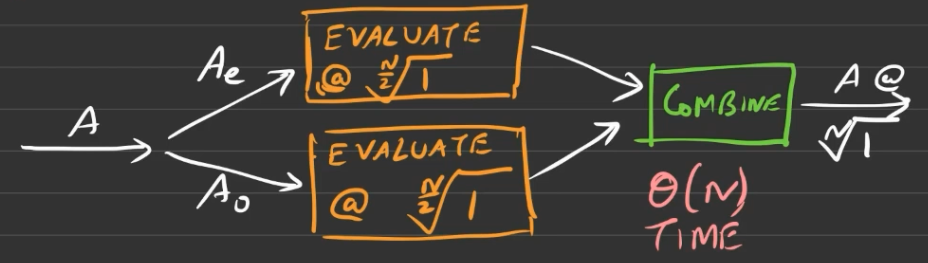
\includegraphics[scale=0.4]{img/fft.png}
    \caption{} 
    \label{fig:fft}
  \end{figure}

  \begin{algo}[Evaluate Nth Degree Polynomial at Nth Roots of Unity]
    
    \begin{algorithm}[H]
      \label{alg:unity}
      \begin{algorithmic}
        \Require{}
        \State 
        \Function{Func}{x}
        \EndFunction
      \end{algorithmic}
    \end{algorithm}
  \end{algo}

  Therefore, we have divided the problem of evaluating over $U(N)$ to be 
  \begin{equation}
    T(N) = 2 T(N/2) + O(N) \implies T(N) = O( N \log{N}) 
  \end{equation}

  So we have shown that in general, evaluating $N$ points of a polynomial takes $O(N^2)$ time, but if you're clever about what points to evaluate, you can get $O(N \log N)$. 

  Now going back to the original problem, we can evaluate $A(u), B(u)$ for $u \in U(N)$, and then multiply them to get $C(u)$. Great. Now to reconstruct the polynomial using the roots of unity, it turns out that there is a method in $O(N \log{N})$ time as well. 


\section{Graph Algorithms}

  A huge portion of problems can be solved by representing as a \textit{graph} data structure. In here, we will explore various problems that can be solved through \textit{graph algorithms}. 

\subsection{Representations and Properties}

  All graphs consist of a set of vertices/nodes $V$ and edges $E$. This tuple is what makes up a graph. We denote $|V| = n, |E| = m$. 

  \begin{definition}[Undirected Graphs]
    An \textbf{undirected graph} $G(V, E)$ is a tuple, where $V = \{v_1, \ldots, v_n\}$ is the vertex set and $E = \{\{v_i, v_j\}\}$ is the edge set (note that it is a set of sets!). 
    \begin{enumerate}
      \item The \textbf{degree} $d_v$ of a vertex $v$ is the number of edges incident to it. 
      \item A \textbf{path} is a sequence of vertices where adjacent vertices are connected by a path in $E$. It's \textbf{length} is the number of edges in the path. 
      \item A \textbf{cycle/circuit} is a path that has the same start and end. 
      \item A graph is \textbf{connected} if for every pair of vertices $e_i, e_j \in E$, there is a path from $e_i$ to $e_j$. 
      \item A \textbf{connected component} is a maximal subset of connected vertices. 
    \end{enumerate}
  \end{definition}

  \begin{definition}[Directed Graph]
    A \textbf{directed graph} $G(V, E)$ is a tuple, where $V = \{v_1, \ldots, v_n\}$ is the vertex set and $E = \{(v_i, v_j)\}$ is the edge set (note that it is a set of tuples, so $(i, j) \neq ( j, i)$).
    \begin{enumerate}
      \item The \textbf{in/out degree} $d_{v, i}, d_{v, o}$ of a vertex $v$ is the number of edges going in to or out from $v$. 
      \item A \textbf{path} is a sequence of vertices where adjacent vertices are connected by a path in $E$. It's \textbf{length} is the number of edges in the path. 
      \item A \textbf{cycle/circuit} is a path that has the same start and end. 
      \item A directed graph is \textbf{strongly connected} if for every pair of vertices $e_i, e_j \in E$, there is a path from $e_i$ to $e_j$.\footnote{Obviously, a connected undirected graph is also strongly connected.}
      \item A \textbf{strongly connected component} is a maximal subset of connected vertices. 
    \end{enumerate}
  \end{definition}

  In fact, from these definitions alone, we can solve an ancient puzzle called \textit{the Bridges of Konigsberg}. Euler, in trying to solve this problem, had invented graph theory. 

  \begin{example}[Bridges of Konigsberg]
    Is there a way to walk that crosses each bridge \textit{exactly} once? 

    \begin{figure}[H]
      \centering
      \begin{subfigure}[b]{0.48\textwidth}
      \centering
        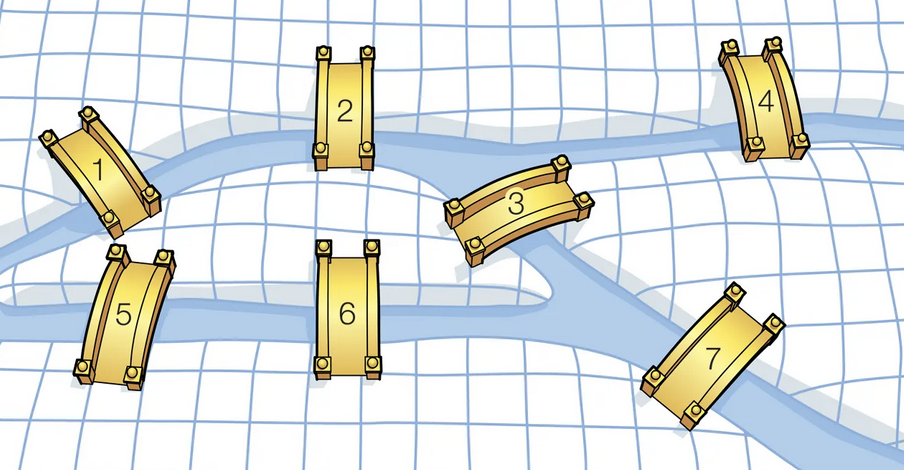
\includegraphics[scale=0.4]{img/bridges.png}
        \caption{Figure of the bridges of Konigsberg.}
        \label{fig:bridges}
      \end{subfigure}
      \hfill 
      \begin{subfigure}[b]{0.48\textwidth}
      \centering
        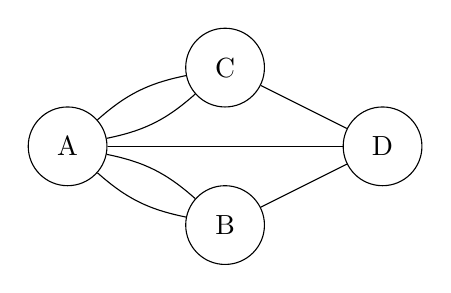
\begin{tikzpicture} 
          \tikzstyle{every node}=[circle, draw, minimum size=1cm]
          
          \node (A) at (0,0) {A};
          \node (B) at (2,-1) {B};
          \node (C) at (2,1) {C};
          \node (D) at (4,0) {D}; 
                
          \draw (A) to[bend left=15] (B);
          \draw (A) to[bend right=15] (B);
          \draw (A) to[bend left=15] (C);
          \draw (A) to[bend right=15] (C);
          \draw (A) -- (D);
          \draw (B) -- (D);
          \draw (C) -- (D);
        \end{tikzpicture}
        \caption{Graph representation. }
        \label{fig:graph_bridges}
      \end{subfigure}
      \caption{It can be decomposed into this undirected graph.}
      \label{fig:konigsberg}
    \end{figure}
     
    Euler's observation is that except for start and end points, a talk leaves any vertex by different edge that the incoming edge. Therefore, the degree (number of edges incident on it) must have an even number, so all but 2 vertices must have an even degree. Since every vertex has an odd degree, there is no way of doing it. 
  \end{example}

  In addition to the \textit{adjacency list} representation, another way in which we represent a directed graph is through \textit{adjacency matrices}. 

  \begin{definition}[Adjacency Matrix]
    In a finite directed graph $(V, E)$, we can construct a bijection from $V$ to the natural numbers and so we label each element in $V$ with $i \in \mathbb{N}$. Then, we can construct a matrix $A$ such that 
    \begin{equation}
      A_{ij} = \begin{cases} 1 & \text{ if } (i, j) \in E \\ 0 & \text{ if } (i, j) \not\in E \end{cases}
    \end{equation}
  \end{definition}

  \begin{example}[Adjacency List vs Matrix]
    Given a graph, we can completely represent it with a list of adjacent vertices for each vertex or an adjacency matrix. 
    \begin{center}
    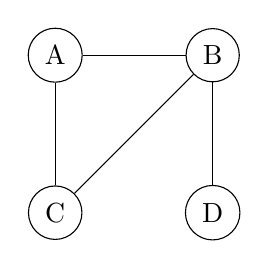
\begin{tikzpicture}
      \node[circle, draw] (C) at (0,0) {C};
      \node[circle, draw] (D) at (2,0) {D};
      \node[circle, draw] (B) at (2,2) {B};
      \node[circle, draw] (A) at (0,2) {A};

      \draw (A) -- (B);
      \draw (B) -- (C);
      \draw (A) -- (C);
      \draw (B) -- (D);
    \end{tikzpicture}
    \end{center}
    An adjacency list would look something like this 
    \[
    \begin{aligned}
    A &: B, C \\
    B &: A, C, D \\
    C &: A, B \\
    D &: B
    \end{aligned}
    \]
    and the adjacency matrix looks like this: 
    \begin{center}
    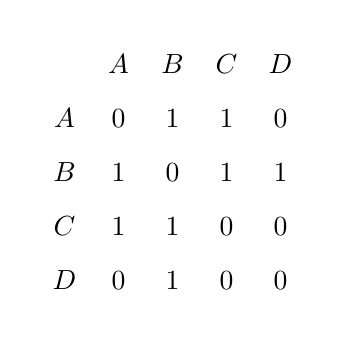
\begin{tikzpicture}
      \matrix[matrix of math nodes, nodes in empty cells,          column sep=-\pgflinewidth, row sep=-\pgflinewidth,          nodes={minimum size=7mm, anchor=center, outer sep=0pt}] (adjacency) {
        & |(a)| A & |(b)| B & |(c)| C & |(d)| D \\
        |(A)| A & 0 & 1 & 1 & 0 \\
        |(B)| B & 1 & 0 & 1 & 1 \\
        |(C)| C & 1 & 1 & 0 & 0 \\
        |(D)| D & 0 & 1 & 0 & 0 \\
      };
    \end{tikzpicture}
    \end{center}
  \end{example}

  While the adjacency matrix does have its advantages and has a cleaner form, usually in sparse graphs this is memory inefficient due to there being an overwhelming number of $0$s. 

  \begin{definition}[Trees]
    An undirected graph $G(V, E)$ is a \textbf{tree} if 
    \begin{enumerate}
      \item $G$ is connected. 
      \item $G$ has no cycles.\footnote{This makes sense, since to get back to a previous vertex you must backtrack.}
    \end{enumerate}
    Removing the first requirement gives us the definition of a \textbf{forest}, which is a collection of trees. Conversely, if $G(V, E)$ is connected  and $|E| = n - 1$, then $G$ is a tree. 
  \end{definition}

  \begin{theorem}[Properties of Trees]
    If $G(V, E)$ is a tree, then 
    \begin{enumerate}
      \item There exists a $v \in V$ s.t. $d_v = 1$, called a \textbf{leaf node}. 
      \item $|E| = |V| - 1 = n - 1$. 
    \end{enumerate}
  \end{theorem}
  \begin{proof}
    The outlines are quite intuitive. 
    \begin{enumerate}
      \item There must be some leaf node since if there wasn't, then we would have a cycle. We can use proof by contradiction. 
      \item We can use proof by induction. We start off with one vertex and to construct a tree, we must add one edge and one vertex at every step, keeping this invariant.  
    \end{enumerate}
  \end{proof}

\subsection{Exploration}

  Given two $v, s \in V$ either directed or undirected, how can we find the shortest path from $v$ to $s$? We can do with either with DFS or BFS. 

  Now, in order to traverse this graph, we basically want to make an algorithm that starts at a node, prints it value, and then goes to all of its neighbors (which we can access through the adjacency list) to print them out. Thus, this is by nature recursive. We don't want the algorithm to loop around printing nodes infinitely often, so we must create a base case that tells the algorithm to not print out a node. It makes sense to create a set of visited nodes, which we can add to whenever we reach a new node. So, if we ever come onto a node that we have visited, we can just tell the function to do nothing. 

  \begin{algo}[Recursive Depth-First Search]
    The recursive implementation of Depth-First Search explores a graph by recursively visiting each unvisited neighbor, going as deep as possible along each branch before backtracking.
    \begin{algorithm}[H]
      \label{alg:dfs_recursive}
      \begin{algorithmic}[1]
        \Require{Graph $G(V, E)$, start vertex $s$}
        
        \Function{DFS-Recursive}{$G, s$}
          \State visited $\gets \emptyset$ \Comment{Initialize empty set of visited vertices}
          \State \Call{DFS-Visit}{$G, s$, visited}
        \EndFunction
        
        \Function{DFS-Visit}{$G, u$, visited}
          \State Add $u$ to visited
          \State \textit{/* Process vertex $u$ here */}
          \For{each neighbor $v$ of $u$ in $G$}
            \If{$v \notin$ visited}
              \State \Call{DFS-Visit}{$G, v$, visited}
            \EndIf
          \EndFor
        \EndFunction
      \end{algorithmic}
    \end{algorithm}
  \end{algo}

  Though recursion really makes this simple, we can construct an iterative approach that uses stacks. Note that in recursion, we are really making a call stack of different functions. We can be explicit about this by actually implementing a stack, which would store all the nodes that we have discovered, but not yet explored from )i.e. all the current nodes). At each iteration, we would pick a node to continue exploring, and since this is a DFS, we would want to implement a LIFO stack so that the last element we input in is the first thing that we should explore from, i.e. we always explore from the last node discovered. 

  \begin{algo}[Iterative Depth-First Search]
    The iterative implementation of Depth-First Search uses a stack to mimic the function call stack of the recursive implementation. It explores vertices in the same order as the recursive version.
    \begin{algorithm}[H]
      \label{alg:dfs_iterative}
      \begin{algorithmic}[1]
        \Require{Graph $G(V, E)$, start vertex $s$}
        
        \Function{DFS-Iterative}{$G, s$}
          \State visited $\gets \emptyset$ \Comment{Initialize empty set of visited vertices}
          \State stack $\gets$ empty stack
          \State Push $s$ onto stack
          \State Add $s$ to visited
          
          \While{stack is not empty}
            \State $u \gets$ Pop from stack
            \State \textit{/* Process vertex $u$ here */}
            
            \For{each neighbor $v$ of $u$ in $G$}
              \If{$v \notin$ visited}
                \State Add $v$ to visited
                \State Push $v$ onto stack
              \EndIf
            \EndFor
          \EndWhile
        \EndFunction
      \end{algorithmic}
    \end{algorithm}
  \end{algo}

  \begin{theorem}[Runtime of DFS]
    The runtime of DFS is $O(n+m)$. 
  \end{theorem}
  \begin{proof}
    The runtime complexity of this search is $O(N + M)$ because first, the while loop loops at most over the $N$ nodes. The for loop may loop over $M$ edges, but this is a bit pessemistic in bound. Rather, we can view it as looping over neighbors of each node at most exactly once, and so it considers every edge twice, meaning that the for loop will get called $2M$ times in the entire algorithm. So $N + 2M = O(N + M)$. 
  \end{proof}

  \begin{example}[DFS in a Maze]
    We can represent a grid graph, like a maze, with a two dimensional array that stores whether it is connected north, east, south, and west, where boolean of true represents that there is a wall, and false means there isn't a wall (so connected). 

    \begin{figure}[H]
      \centering
      \begin{subfigure}[b]{0.48\textwidth}
      \centering
        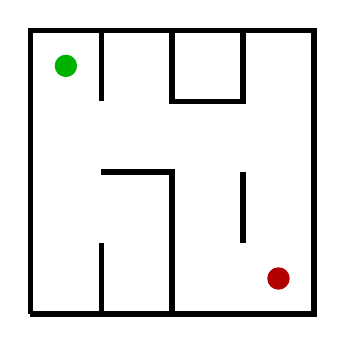
\begin{tikzpicture}[scale=0.9]
          % Outer boundary
          \draw[line width=2pt] (0,0) -- (4,0) -- (4,4) -- (0,4) -- (0,0);
          
          % Internal walls
          % Top section
          \draw[line width=2pt] (1,4) -- (1,3);
          \draw[line width=2pt] (2,4) -- (2,3) -- (3,3) -- (3,4);
          
          % Middle section
          \draw[line width=2pt] (1,2) -- (2,2) -- (2,1);
          \draw[line width=2pt] (3,2) -- (3,1);
          
          % Bottom section
          \draw[line width=2pt] (1,1) -- (1,0);
          \draw[line width=2pt] (2,1) -- (2,0);
          
          % Entry and exit points (just colored circles)
          \filldraw[green!70!black] (0.5,3.5) circle (0.15);
          \filldraw[red!70!black] (3.5,0.5) circle (0.15);
        \end{tikzpicture}
        \caption{4×4 maze representation}
        \label{fig:maze}
      \end{subfigure}
      \hfill 
      \begin{subfigure}[b]{0.48\textwidth}
      \centering
        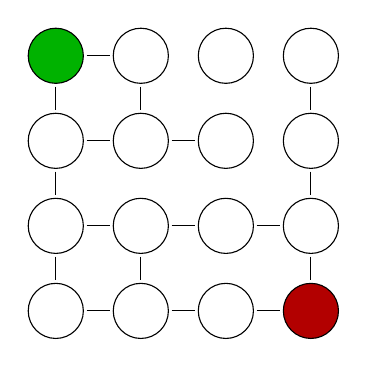
\begin{tikzpicture}[
          scale=0.9,
          node/.style={circle, draw, minimum size=0.7cm},
          edge/.style={draw, -, shorten >=1pt, shorten <=1pt}
        ]
          % Create a 4x4 graph for the new maze
          % Top row
          \node[node, fill=green!70!black, text=white] (A) at (0,3.6) {};
          \node[node] (B) at (1.2,3.6) {};
          \node[node] (C) at (2.4,3.6) {};
          \node[node] (D) at (3.6,3.6) {};
          
          % Second row
          \node[node] (E) at (0,2.4) {};
          \node[node] (F) at (1.2,2.4) {};
          \node[node] (G) at (2.4,2.4) {};
          \node[node] (H) at (3.6,2.4) {};
          
          % Third row
          \node[node] (I) at (0,1.2) {};
          \node[node] (J) at (1.2,1.2) {};
          \node[node] (K) at (2.4,1.2) {};
          \node[node] (L) at (3.6,1.2) {};
          
          % Bottom row
          \node[node] (M) at (0,0) {};
          \node[node] (N) at (1.2,0) {};
          \node[node] (O) at (2.4,0) {};
          \node[node, fill=red!70!black, text=white] (P) at (3.6,0) {};
          
          % Add edges based on available paths in the maze
          % Vertical connections
          \draw[edge] (A) -- (E);
          \draw[edge] (E) -- (I);
          \draw[edge] (I) -- (M);
          
          \draw[edge] (B) -- (F);
          
          \draw[edge] (D) -- (H);
          \draw[edge] (H) -- (L);
          \draw[edge] (L) -- (P);
          
          \draw[edge] (J) -- (N);
          
          % Horizontal connections
          \draw[edge] (A) -- (B);
          
          \draw[edge] (E) -- (F);
          \draw[edge] (F) -- (G);
          
          \draw[edge] (I) -- (J);
          \draw[edge] (J) -- (K);
          \draw[edge] (K) -- (L);
          
          \draw[edge] (M) -- (N);
          \draw[edge] (N) -- (O);
          \draw[edge] (O) -- (P);
        \end{tikzpicture}
        \caption{Graph representation of the maze.}
        \label{fig:maze-graph}
      \end{subfigure}
      \caption{A 4×4 maze (left) and its corresponding graph representation (right). Start and end points are shown in green and red respectively.}
      \label{fig:maze-and-graph}
    \end{figure}

    But remember that in a tree traversal, we recursively searched down and down until we hit a null node, in which case we backtrack up to look in another branch. For graphs, this is a bit more complicated, since we could go in loops. Therefore, we want to keep track of all the visited nodes to avoid infinite recursion. We have three base cases: 
    \begin{enumerate}
      \item If we search off the grid, then this is not a valid path 
      \item If we already explored here, then we don't want to repeat it 
      \item If we reached the goal of the maze, then we output the length of the path. 
    \end{enumerate}
    The recursive case would take each node and recurse on its 4 adjacent neighbors, if they are connected. Note that this algorithm recurses on each of the $N$ nodes $4$ times (for each direction, and each recursive call is $O(1)$), so the complexity is $O(N)$. 
  \end{example}

  Note that the main idea of DFS is to always explore a new adjacent vertex if possible, and if not, then backtrack to the most recent vertex adjacent to an unvisited vertex and continue. On the contrary, the main idea of BFS is to explore \textit{all} your neighbors before you visit any of your neighbors' neighbors. It exhaustively searches for the closest regions of your search space before you look any further. Unlike DFS, which finds the some arbitrary path to a node, BFS finds the shortest (perhaps non-unique) path to a node. This can be simply done with a queue. 

  \begin{algo}[Iterative Breadth-First Search]
    Breadth-First Search (BFS) explores a graph by visiting all neighbors at the current depth before moving to nodes at the next depth level. It uses a queue to process nodes in the order they are discovered.
    \begin{algorithm}[H]
      \label{alg:bfs}
      \begin{algorithmic}[1]
        \Require{Graph $G(V, E)$, start vertex $s$}
        
        \Function{BFS}{$G, s$}
          \State visited $\gets \emptyset$ \Comment{Initialize empty set of visited vertices}
          \State queue $\gets$ empty queue
          \State Enqueue $s$ onto queue
          \State Add $s$ to visited
          
          \While{queue is not empty}
            \State $u \gets$ Dequeue from queue \Comment{Get the next vertex to process}
            \State \textit{/* Process vertex $u$ here */}
            
            \For{each neighbor $v$ of $u$ in $G$}
              \If{$v \notin$ visited}
                \State Add $v$ to visited
                \State Enqueue $v$ onto queue
              \EndIf
            \EndFor
          \EndWhile
        \EndFunction
      \end{algorithmic}
    \end{algorithm}
  \end{algo}

  \begin{theorem}[Runtime of BFS]
    The runtime of BFS is $O(n+m)$. 
  \end{theorem}
  \begin{proof}
    To get the running time, we know that each vertex is popped only once from the queue, giving us $O(n)$. For each pop, we are exploring all the neighbors of $V$. 
    \begin{align}
      O \bigg( \sum_{v \in V} | \text{neighbors of } v| + 1\bigg) & = O \bigg( \sum_{v \in V} d_v + 1 \bigg) \\
                                           & = O (2 |E| + |V|) = O(m + n )
    \end{align}
    which is linear in input size!  
  \end{proof}

  The more straightforward application is in reachability. 

  \begin{example}[Reachability]
    Given a directed graph and a node $v$, find all nodes that are reachable from $v$. 
  \end{example}

  \begin{exercise}
    Prove that in any connected undirected graph $G = (V, E)$ there is a vertex $v \in V$ s.t. $G$ remains connected after removing $v$. 
  \end{exercise}
  \begin{proof}
    Let $u$ be such a leaf node of $T$, and let $G'$ be the subgraph of $G$ resulting by removing $u$ and its incident edges from $G$.
    For sake of contradiction,\footnote{We provide an alternative direct proof as follows: Since $G$ is given to be connected, $T$ contains all vertices of $G$. Let $T'$ be the BFS tree minus $u$ and its single incident edge connecting it to its parent in $T$. Since $u$ is a leaf, $T'$ remains a connected tree with all other vertices of $G$. The edges of $T'$ exist in $G'$, so $G'$ is connected.} suppose $G'$ has more than one connected component.
    Let $C$ be a connected component in $G'$ that does not contain $s$, the root of the BFS tree $T$.
    Since $G$ was connected before the removal of $u$, it must be that every path from $s$ to any vertex $v$ in $C$ includes $u$ (otherwise there would remain a path from $s$ to $v$ in $G'$ and $s$ would be in $C$).
    Then $u$ is the only vertex not in $S$ with edges to vertices in $S$, so all vertices in $C$ must be ``visited'' during BFS only after visiting $u$. Furthermore, the vertices of $S$ must be in the subtree of $T$ rooted at $u$. But $u$ is a leaf, which is a contradiction.
  \end{proof}

  \begin{exercise}
    Two parts. 
    \begin{enumerate}
      \item Give an example of a strongly connected directed graph $G = (V, E)$ s.t. that every $v \in V$, removing $v$ from $G$ gives a directed graph that is not strongly connected. 
      \item In an undirected graph with exactly two connected components, it is always possible to make the graph connected by adding only one edge. Give an example of a directed graph with two strongly connected components such that no addition of one edge can make the graph strongly connected.
    \end{enumerate}
  \end{exercise}
  \begin{proof}
    Listed. 
    \begin{enumerate}
      \item A graph whose edges form a cycle, having at least three nodes.
      \item Two strongly connected components with no edges between them.
    \end{enumerate}
  \end{proof} 

  \begin{definition}[Search Trees]
    Once we have traversed a graph using BFS or DFS, we can label the directed path that this traversal algorithm takes into a \textbf{search tree}. 

    \begin{figure}[H]
      \centering
      \begin{subfigure}[b]{0.48\textwidth}
      \centering
        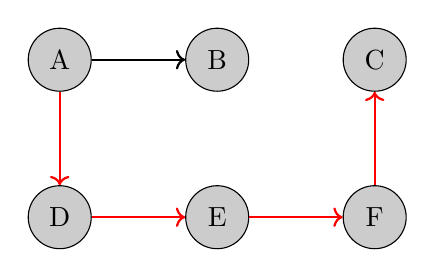
\begin{tikzpicture}[
            node/.style={circle, draw, fill=gray!40, minimum size=0.8cm},
            edge/.style={->, thick}
        ]
        % Create nodes
        \node[node] (A1) at (0,2) {A};
        \node[node] (B1) at (2,2) {B};
        \node[node] (C1) at (4,2) {C};
        \node[node] (D1) at (0,0) {D};
        \node[node] (E1) at (2,0) {E};
        \node[node] (F1) at (4,0) {F};
        
        % Create edges
        \draw[edge] (A1) -- (B1);
        \draw[edge, red, thick] (A1) -- (D1);
        \draw[edge, red, thick] (D1) -- (E1);
        \draw[edge, red, thick] (E1) -- (F1);
        \draw[edge, red, thick] (F1) -- (C1);
        \end{tikzpicture}
        \caption{After DFS traversal, we can store the previous nodes in a hashmap $\{B \mapsto A, D \mapsto A, E \mapsto D, F \mapsto E, C \mapsto F\}$. From this we can see the path to get to $C$ is $A \mapsto D \mapsto E \mapsto F \mapsto C$ of length 4. }
        \label{fig:graph1}
      \end{subfigure}
      \hfill 
      \begin{subfigure}[b]{0.48\textwidth}
      \centering
        \begin{tikzpicture}[
            node/.style={circle, draw, fill=gray!40, minimum size=0.8cm},
            edge/.style={->, thick}
        ]
        % Create nodes
        \node[node] (A2) at (0,2) {A};
        \node[node] (B2) at (2,2) {B};
        \node[node] (C2) at (4,2) {C};
        \node[node] (D2) at (0,0) {D};
        \node[node] (E2) at (2,0) {E};
        \node[node] (F2) at (4,0) {F};
        
        % Create edges
        \draw[edge, red, thick] (A2) -- (B2);
        \draw[edge] (A2) -- (D2);
        \draw[edge] (B2) -- (E2);
        \draw[edge, red, thick] (B2) -- (F2);
        \draw[edge, red, thick] (F2) -- (C2);
        \end{tikzpicture}
        \caption{After BFS traversal, we can store the previous nodes in a hashmap $\{B \mapsto A, D \mapsto A, E \mapsto B, F \mapsto B, C \mapsto F\}$. From this we can see the path to get to $C$ is $A \mapsto B \mapsto F \mapsto C$ of length 3. }
        \label{fig:graph2}
      \end{subfigure}
      \caption{Comparison of two directed graphs with different path lengths from A to C.}
      \label{fig:graph-comparison}
    \end{figure}

    By construction, we can see that the path from A to C is always shorter for BFS than for DFS. 
  \end{definition}

\subsection{Directed Acyclic Graphs and Topological Sorting}

  \begin{definition}[Directed Acyclic Graph]
    A DAG is a directed graph that has no cycles. Note that a DAG must have a node that has no in-edges. 
  \end{definition}

  To determine if a graph is a DAG, then we can brute force it by taking a node $s \in V$, running DFS/BFS, and if a neighbor is already in visited, return False. Then go through this for all starting nodes $s \in V$. This again has quadratic runtime. Can we do better? This introduces us to topological sorting. 

  It may be helpful to take a graph $G(V, E)$ and induce some partial order on the set of nodes $V$ based off of $E$. It turns out that we can do this for a specific type of graph. 
  
  \begin{definition}[Topological Sort]
    Given a directed acyclic graph (DAG), a linear ordering of vertices such that for every directed edge $u-v$, vertex $u$ comes before $v$ in the ordering is called a \textbf{topological sort}. It satisfies the facts: 
    \begin{enumerate}
      \item The first vertex must have an in-degree of $0$. 
      \item A topological sort is not unique. 
    \end{enumerate}

    \begin{figure}[H]
      \centering
      \begin{subfigure}[b]{0.48\textwidth}
      \centering
        \begin{tikzpicture}[
            scale=0.8, 
            node/.style={circle, draw, thick, minimum size=1.0cm}, 
            edge/.style={->, black, thick}
        ]

        % Center node
        \node[node] (n0) at (0,0) {0};

        % Upper nodes
        \node[node] (n5) at (-1.5,1.5) {5};
        \node[node] (n4) at (1.5,1.5) {4};

        % Lower nodes
        \node[node] (n2) at (-2,-1.5) {2};
        \node[node] (n1) at (2,-1.5) {1};
        \node[node] (n3) at (0,-2.5) {3};

        % Directed edges
        \draw[edge] (n5) -- (n0);
        \draw[edge] (n4) -- (n0);
        \draw[edge] (n5) -- (n2);
        \draw[edge] (n4) -- (n1);
        \draw[edge] (n2) -- (n3);
        \draw[edge] (n1) -- (n3);
        \end{tikzpicture}
        \caption{This graph can have the two (not exhaustive) topological sortings $[5, 4, 2, 3, 1, 0]$ and $[4, 5, 2, 3, 1, 0]$.}
        \label{fig:top_sort_not_unique}
      \end{subfigure}
      \hfill 
      \begin{subfigure}[b]{0.48\textwidth}
      \centering
        \begin{tikzpicture}[
            scale=0.8,
            node/.style={circle, draw, thick, minimum size=1.0cm},
            edge/.style={->, black, thick}
        ]

        % Center and bottom nodes
        \node[node] (n3) at (0,0) {3};
        \node[node] (n5) at (0,-2) {5};

        % Left side nodes
        \node[node] (n1) at (-2,1) {1};
        \node[node] (n2) at (-1.5,-1) {2};

        % Right side nodes
        \node[node] (n4) at (2,1) {4};
        \node[node] (n6) at (1.5,-1) {6};

        % Directed edges ensuring unique topological order
        \draw[edge] (n1) -- (n2);
        \draw[edge] (n1) -- (n3);
        \draw[edge] (n1) -- (n4);
        \draw[edge] (n2) -- (n5);
        \draw[edge] (n3) -- (n5);
        \draw[edge] (n3) -- (n6);
        \draw[edge] (n4) -- (n6);
        \draw[edge] (n2) -- (n6);

        \end{tikzpicture}
        \caption{This graph can have the two (not exhaustive) topological sortings $[1, 4, 2, 3, 6, 5]$ and $[1, 4, 3, 2, 6, 5]$.}
        \label{fig:top_sort_unique}
      \end{subfigure}
      \caption{Examples of topological sortings of different graphs. }
      \label{fig:top_sort}
    \end{figure}
  \end{definition}

  To determine if a graph is a DAG, note the following theorem. 

  \begin{theorem}[Topological Order and DAGs]
    $G$ has a topological order if and only if it is a DAG. 
  \end{theorem}
  \begin{proof}
    To prove that a DAG has a topological order, we use induction. Pick a $v$ such that its indegree is $0$. Then, delete $v$, and therefore $G \setminus v$ is also a DAG with a topological order since we are only deleting edges. We keep going. 
  \end{proof}

  Therefore, if we can successfully topologically sort, we know it is a DAG. So we can kill two birds with one stone. Let's see how this is implemented. We can do it iteratively and recursively (the proof above should hint that this can be recursive). 

  \begin{algo}[Iterative Topological Sort, Determine If Graph is DAG]
    The general idea is that we first find the node that as $0$ in-degree. From here, we can do DFS, and when we run out of neighbors to explore, then we push this into a queue. This is essentially a post-order traversal, where at the end are going to be the end nodes with no more neighbors, and the node we started from will be added last. Then we loop through and do this for all start nodes. We first need a slightly modified form of DFS. 

    \begin{algorithm}[H]
      \label{alg:iterative_top_sort}
      \begin{algorithmic}[1]
        \Require{Nodes $V$, adjacency list $E$}
        \State visited $\gets$ set()
        \State res $\gets$ stack() 
        \State is\_acyclic $\gets$ True

        \Function{DFS}{$v \in V$}
          \If{$v \neq $ visited}
            \State add $v$ to visited 
            \State $N_v \gets$ neighbors of $v$ 
            \For{$n \in N_v$}
              \If{$n \in $ visited} 
                \State is\_acyclic $\gets$ False 
              \EndIf
              \State \Call{DFS}{$n$}
            \EndFor 
            \State push $v$ onto res
          \EndIf
        \EndFunction

        \State 

        \Function{TopologicalSort}{V, E}
          \For{$v \in V$} 
            \State DFS($v$)
          \EndFor
          \If{! is\_acyclic}
            \State \Return{False}
          \EndIf
          \State \Return{reversed of res}
        \EndFunction
      \end{algorithmic}
    \end{algorithm}
    Note that this runtime is $O(|V| + |E|)$ since we are just running DFS with a constant amount of work on top of each call. 
  \end{algo}

  \begin{algo}[Recursive Topological Sort]
    We want to see that while $G$ is nonempty, we want to find the $v \in V$ such that it has indegree $0$. Then place $v$ next in order, and then delete $v$ and all edges out of $v$. The problem is finding which vertex has indegree $0$ (if we brute force it by looking through all remaining nodes and edges, you have quadratic runtime). To do this fast, the idea is 
    \begin{enumerate}
      \item initially scan over all edges to store the indegrees of every node to a list \texttt{indeg}. 
      \item store all nodes with indegree $0$ to a queue. 
      \item Run through the queue, and during each loop, when we remove a node, we look at all of its out-nodes $s$ and decrement \texttt{indeg[s]}. If \texttt{indeg[s] = 0}, then add it to the queue. 
    \end{enumerate}
    \begin{algorithm}[H]
      \label{alg:recursive_top_sort}
      \begin{algorithmic}[1]
        \Require{Nodes $V$, Edges $E$}
        \State $q \gets$ queue() 
        \State indeg $\gets$ list() 
        \State visited $\gets$ 0
        \Function{Recur}{x}
          \State initialize the indeg and $q$ 

          \While{q is nonempty} 
            \State $v \gets$ pop(q) 
            \State visited += 1 
            \For{each $w \in E[v]$} 
              \State indeg[w] -= 1 
              \If{indeg[w] = 0} 
                \State push w into q 
              \EndIf
            \EndFor
          \EndWhile

          \If{visited != |V|} 
            \State \Return{False}
          \EndIf

          \State \Return{True}
        \EndFunction
      \end{algorithmic}
    \end{algorithm}
    Notice that the inner for loop is $O(d(v) + 1)$, while we run over all $n$. So really, we are doing $O(n(d(v) + 1)) = O(m + n)$, where the plus $n$ comes from the constant work we are doing for each node. Note that if we have a non-DAG, then at some point the queue will be empty but we haven't processed all the vertices, at which point we can declare failure. 
  \end{algo}

  To end this, we can make a general statement about all directed graphs. 

  \begin{theorem}
    Every directed graph is a DAG of strongly connected components (SCC). 
  \end{theorem}

  This gives us a way to represent a directed graph with a collection of DAGs.\footnote{In fact, this Kosaraju's algorithm, can be done in linear time, though it is highly nontrivial.} An extension of topological sort is making a \textit{BFS tree}, which partitions a graph into layers that represent the number of steps required to go from a source vertex to a node. 

  \begin{algo}[BFS Tree]
    To construct a BFS tree, we just need to slightly modify the original BFS code.
    \begin{algorithm}[H]
      \label{alg:bfs_tree}
      \begin{algorithmic}[1]
        \Require{Nodes $V$, adjacency list $E$}
        \State visited = set() 
        \State layers = $\{v : 0 \mid v \in V \}$
        \Function{BFS}{start}
          \State layer $\gets 0$ 
          \State toExplore $\gets$ queue() 
          \State add (start, layer) to toExplore 
          \State add start to visited
          \While{toExplore} 
            \State curr, layer = pop from toExplore 
            \State layers[curr] = layer 
            \For{$n \in$ neighbors of curr} 
              \If{$n \not\in$ visited} 
                \State add $n$ to visited 
                \State add $(n, layer+1)$ to visited 
              \EndIf
            \EndFor
          \EndWhile 
        \EndFunction
      \end{algorithmic}
    \end{algorithm}
    This is simply BFS with constant extra work so it is $O(n + m)$. 
  \end{algo}

  So, a BFS tree is really just another way to topologically sort. Note the following properties. 
  \begin{enumerate}
    \item In a directed graph, no nodes can jump from layer $i$ to layers $j > i+1$, since if it could, then it would be in layer $i+1$. However, nodes can jump from layer $j$ back to any layer $i < j$, even skipping layers. 
    \item In a directed graph, going forward is the same as going back, so nodes can jump at most one layer forwards or backwards. 
  \end{enumerate}


  \begin{exercise}[DPV 3.16]
    Suppose a CS curriculum consists of $n$ courses, all of them mandatory. The prerequisite graph $G = (V,E)$ has a node for each course, and an edge from course $v$ to course $w$ if and only if $v$ is a prerequisite for $w$. Note this is a directed acyclic graph (DAG). In order for a student to take a course $w$ with prerequisite $v$, they must take $v$ in an earlier semester. Find an algorithm that works directly with this graph representation, and computes the minimum number of semesters necessary to complete the curriculum, under the assumption any number of courses can be taken in one semester. The running time of your algorithm should be $O(n+m)$, where $n$ and $m$ are the numbers of vertices and edges in $G$, respectively.
  \end{exercise}
  \begin{proof}
    For each vertex, we want to find the longest path leading to it: if there is a path leading to a node, then all of the courses in the path should be taken sequentially. Perform a topological sort of $G$'s nodes and label them $1$ through $n$. Then, we go through the nodes in the resulting topological order. For each vertex, we assign the minimum number of semesters required to take it: if there are no prerequisites, we assign 1, and if there are prerequisites, we assign 1 plus the maximum value assigned to its prerequisite nodes.
    
    \textit{Implementation details}: If the input is in adjacency list format, then we do not have access to the \emph{incoming} edges to a node (its prerequisites). By exploring the entire graph with BFS calls, we can compute the list of incoming edges to every vertex in $O(n+m)$ time. These details are not required. If the input is in adjacency matrix format, for each node it takes $O(n)$ time to find its incoming edges, so the total running time is $O(n^2)$.
  \end{proof}

  \begin{exercise}[DPV 3.22] 
    Give an efficient algorithm that takes as input a directed graph $G = (V,E)$, and determines whether or not there is a vertex $s \in V$ from which all other vertices are reachable.
  \end{exercise}
  \begin{proof}
    We first build the DAG representation of the SCCs of $G$ in $O(m+n)$ time, as described in lecture. This graph is a DAG where each SCC of $G$ is represented by a single node. We return true if this DAG has exactly one node with no incoming edges (i.e., exactly one source node), and return false otherwise.

    \textit{Correctness.} Let $u$ be a vertex in an SCC that is a source node in the DAG representation. If there is a path in $G$ from a vertex $v$ not in the SCC of $u$ to $u$, then there must be an edge (corresponding to an edge in this path) into the SCC of $u$ in the DAG, which contradicts that the node has no incoming edges. Thus, if there are two source SCCs in the DAG, no vertex of $G$ can reach all vertices; in particular, no vertex can reach the vertices in both of the source SCCs. Thus we correctly return false if there are multiple source SCCs. 
    
    On the other hand, if there is a single source SCC in the DAG, we claim that every vertex in the SCC can reach every other vertex in $G$, in which case our algorithm correctly returns true. Every other SCC in the DAG is not a source, so it has an incoming edge.\footnote{The following argument can be made formal with induction.} Consider starting at an SCC in the DAG, picking an incoming edge to the SCC, and then repeating this process from the SCC from which the edge was leaving. This process stops when we reach an SCC without incoming edges. In this case there is exactly one source SCC, so this process will arrive at the single source SCC when starting from any SCC in the DAG. This implies there is a path from the unique source SCC to every other SCC in the DAG, and thus every vertex of the source SCC can reach all vertices in all SCCs of $G$; that is, all vertices of $G$.
  \end{proof}

  \begin{exercise}[DPV 3.19]
    You are given a binary tree $T = (V, E)$ with designated root node with $n = |V|$ vertices which are the integers from $1$ to $n$. In addition, there is an array $x[1..n]$ of values where $x[u]$ is the value of vertex $u \in V$. Define a new array $z[1..n]$ where, for each $u \in V$,	
    \begin{equation}
      z[u] = \max \{ x[v] \mid \text{$v$ is a descendant of $u$}\}
    \end{equation}
    That is, $z[u]$ is the maximum $x$-value of all vertices in the subtree of $T$ rooted at $u$. Note that, by definition, any node is a descendant of itself. Describe an $O(n)$-time algorithm which calculates the entire $z$-array.
  \end{exercise}
  \begin{proof}
    We propose the following recursive algorithm performs a \emph{postorder} traversal of the tree and populates the values of the $z$-array in the process:
    \begin{lstlisting}
      computeZ(u):
        maxVal = x[u]
        if u.left is not null:
          computeZ(u.left) # compute z for all descendants of u.left
          maxVal = max(z[u.left], maxVal)
        if u.right is not null:
          computeZ(u.right) # computes z for all descendants of u.right
          maxVal = max(z[u.right], maxVal)
        z[u] = maxVal
    \end{lstlisting}
    We initially call \texttt{computeZ} on the root node of $T$.        The algorithm takes $O(1)$ time per node, which is $O(n)$ overall\footnote{This algorithm can also be described as a modified version of the so-called \emph{depth-first search} (DFS) graph traversal algorithm, which is different from BFS.}
  \end{proof}

  \begin{exercise}
    Your data center needs to run a number of jobs (compute requests) numbered $1, 2, \dots, n$. These are specified in a list of $m$ tuples where $(i, k)$ means that job $i$ must be completed before job $k$ can run. A given job may have multiple dependencies; for example, you might have constraints $(1, 4), (2, 4), (3, 4)$ that all of jobs $1, 2, \mbox{ and } 3$ must be completed before $4$ can run.
    \begin{enumerate}
      \item Describe an $O(n+m)$ runtime algorithm that determines whether it is possible to execute all of the jobs, and if so, determines a valid order in which to execute the jobs one at a time. \textit{Hint. How to relate SCCs to cycles?}
      \item Suppose you have $n$ identical servers (so that if there were no constraints you could simply run each job on a separate server). Suppose every job has the same runtime $R$. Describe an $O(n+m)$ runtime algorithm to compute the total runtime that will be necessary to run all of the jobs in a valid order.
    \end{enumerate}
  \end{exercise}
  \begin{proof}
    For this question we define a graph $G = (V, E)$ where there is a vertex for every job $1, \dots, n$ and an edge from $i$ to $k$ for every listed dependency (where $k$ depends on $i$).

    \begin{enumerate}
        \item We note that a sequence of jobs can be executed if and only if there is no circular dependency. In the language of graphs, this requires that $G$ be free of cycles. To this end, it suffices to propose an algorithm that runs in $\mathcal{O}(m+n)$. We will use Kosaraju's SCC algorithm. We prove the following claim:

        \centerline{Any SCC with $\geqslant 2$ vertices contain a cycle.}
                    \vspace{5pt} 
  
        To see this, consider any distinct $u,v$ in this SCC. Let $p_{u,v}$ and $p_{v,u}$ be the paths from $u$ to $v$ and backwards, respectively. Now concatenate the paths and get a walk that starts from $u$ and ends at $u$. Note that each vertex appears at most once in $p_{u,v}$ and in $p_{v,u}$, so in the combined walk, it appears at most twice. Consider the set of vertices that are revisited in this walk --- clearly, $u$ is one of them and is the latest one to be revisited. There must exist a vertex $w$ that was the \textit{first} to be revisited. Then, the section of the walk between the two visits of $w$ form a cycle by definition: it starts from $w$, ends at $w$, and does not repeat any other vertices. This proves the claim. And to go back to our problem, the following are equivalent: 
        \begin{enumerate}
          \item jobs can be executed 
          \item no cycles in $G$ 
          \item each SCC obtained from Kosaraju is a singleton
        \end{enumerate}

        \item We first run the algorithm from part (a) to check if it is possible and to find a valid order of the jobs if so. Then define an array $L$ of length $n$. We will compute $L[k]$ as the length of the longest dependency chain prior to $k$. Loop over the $k$ jobs in topological order. For each, compute $L[k] = 0$ if $k$ has no dependencies, or $L[k] = 1 + \max_{(i, k)} L[i]$ otherwise. Finally, return $\max_{k} L[k]$. 
    \end{enumerate}
    
  \end{proof}

\subsection{Bipartite Graphs}

  Now we shall see a further application of BFS trees. 

  \begin{definition}[Bipartite Graph]
    A \textbf{bipartite graph} is an undirected graph $G(V, L)$ where we can partition $V = L \sqcup R$ such that for all $e = \{u, v\} \in E$, we have $u \in L, v \in R$.  
  \end{definition}

  We would like to devise some method to determine if an arbitrary graph is bipartite. 

  \begin{theorem}
    $G$ is bipartite if and only if all cycles in $G$ are even length. 
  \end{theorem}
  \begin{proof}
    Proving $(\implies)$ is quite easy since if we suppose $G$ has an odd length cycle, then we start packing vertices of a cycle into $L, R$, but by the time we came back to the start, we are forced to pack it into the wrong partition! 

    The converse is quite hard to prove, and we'll take it at face value. 
  \end{proof}

  Now in practice, how would we determine if all cycles are even length? This is where BFS shines. 

  \begin{algo}[Determine Bipartite On All Cycles of Even Length]
    The general idea is we first run BFS on the graph starting at $s \in V$, which divides it up into layers $L_1, \ldots, L_l$ representing the shortest path from $s$. Then for each layer $L_i \subset V$, we check if there are connections between two vertices $x, y \in L_i$. If there are connections, then this is not bipartite. If there are none, then this is bipartite since we can then color it. 

    \begin{algorithm}[H]
      \label{alg:determine_bipartite}
      \begin{algorithmic}[1]
        \Require{Nodes $V$, adjacency list $E$}
        \State visited = set() 
        \State layers = $\{v : 0 \mid v \in V \}$
        \Function{BFS}{start}
          \State layer $\gets 0$ 
          \State toExplore $\gets$ queue() 
          \State add (start, layer) to toExplore 
          \State add start to visited
          \While{toExplore} 
            \State curr, layer = pop from toExplore 
            \State layers[curr] = layer 
            \For{$n \in$ neighbors of curr} 
              \If{$n \not\in$ visited} 
                \State add $n$ to visited 
                \State add $(n, layer+1)$ to visited 
              \EndIf
            \EndFor
          \EndWhile 
        \EndFunction

        \State 

        \Function{Bipartite}{V, E}
          \State BFS(v) for some $v \in V$ 
          \For{$(u, v) \in E$} 
            \If{layers[u] == layers[v]} 
              \State \Return{False} 
            \EndIf 
          \EndFor 
          \State \Return{True}
        \EndFunction
      \end{algorithmic}
    \end{algorithm}
    Therefore, we run BFS, which is $O(n+m)$, and then to compare the edges, it is $O(m)$. 
  \end{algo}

  Bipartiteness is actually a special case of \textit{coloring problems}. Given a graph with $k$ colors, can I color it so that every neighbor has a different color than the original node? It may seem like at first glance that we can do the same method and look at the layers again, but it turns out that 3-coloring is hard. More specifically it is an NP-complete problem, which colloquially means that there isn't much of a better way than a brute-force solution. However, it turns out that according to the \textit{4 color theorem}, any map can be colored with 4 colors. 

\subsection{Strongly Connected Graphs}

  Now how do we find out if a directed graph is strongly connected? The straightforward solution would be to take each vertex $v \in V$, run BFS to find the set of vertices reachable from $v$, and do this for every vertex. The total running time is $O(n(n+m))$, which is quadratic. Note that for an undirected graph this is trivial since we just run DFS/BFS once. 

  \begin{theorem}
    $G$ is strongly connected if and only if for any $v \in V$, 
    \begin{enumerate}
      \item all of $V$ is reachable from $v$. 
      \item $v$ is reachable from any $s \in V$
    \end{enumerate}
  \end{theorem}

  \begin{algo}[Determine if Graph is Strongly Connected]
    Using the theorem above, we can run BFS/DFS twice: one on the original graph and one on the reversed graph, consisting of all edges directed in the opposite direction. 
    \begin{algorithm}[H]
      \label{alg:strongly_connected}
      \begin{algorithmic}[1]
        \Require{Nodes $V$, Adjacency list $E$}
        \Function{StronglyConnected}{$s \in V$}
          \State visited $\gets$ set() 
          \State BFS(s) 
          \If{visited != $V$} 
            \State \Return{False}
          \EndIf
          \State visited $\gets$ set() 
          \State reverse all edges in $E$ 
          \State BFS(s) 
          \If{visited != $V$} 
            \State \Return{False}
          \EndIf
          \State \Return{True}
        \EndFunction
      \end{algorithmic}
    \end{algorithm}
    The running time is just running BFS twice plus the time to reverse the edges, so it is $O(n+m)$. 
  \end{algo}

\subsection{Shortest Path}

  In the shortest path, you are given a \textit{weighted} (positive integer) directed graph and your goal is to find a path from $s$ to $t$ with the smallest length. This is where we use Dijkstra's. What we can do to brute force is just replace a edge with length $k$ to $k$ edges of length $1$, and we run BFS on this. However, this is not efficient since the weights can be unbounded. This is where we introduce Dijkstra. The following is how it is introduced in class. 

  \begin{algo}[General Dijkstra]
    We can keep a temporarily list $\pi$ of the shortest path we have found so far, and a permanent list \texttt{dist} keeping track of all paths we know are for sure the shortest path. 
    \begin{algorithm}[H]
      \label{alg:dik_in_class}
      \begin{algorithmic}[1]
        \Require{Graph $G(E, V)$}
        \State $S \gets \{s\}$  \Comment{set of nodes that we know for sure is shortest}
        \State dist[s] = 0 and the rest very large numbers \Comment{our final list}
        \State $\pi[v] = w_{sv}$ for all $v \in V$ \Comment{initialize list with neighboring nodes from start $s$}
        \Function{Dijkstra}{s}
          \State $u = \mathrm{argmin}_{v \notin S} \pi[v]$ \Comment{Find node having minimum accum weight so far}
          \State add $u$ to $S$ \Comment{This node must be shortest so add to $S$}
          \State $\mathrm{dist}[u] = \pi[u]$ \Comment{Now we can update its shortest path in dist}
          
          \For{$v \not\in S$} \Comment{Look at all neighbors of $u$ and update those not in}
            \State $\pi[v] \gets \min\{\pi[v], d[u] + w_{wv}\}$ \Comment{$S$ since those in $S$ are all guaranteed to be shortest}
          \EndFor
        \EndFunction
      \end{algorithmic}
    \end{algorithm}
  \end{algo}

  The problem is line 5 above. We don't want this linear search time since it makes the whole thing quadratic, so rather than a list, we can implement a heap, resulting in the code below. 

  \begin{algo}[Dijkstra's Algorithm]
    The general idea is to run a graph traversal like BFS but when you reach a new vertex $v$, you can store the accumulated time it took to get to $v$ and store for all neighbors the accumulated time it will take to get to each of those neighbors. If it is less than what we have currently, then we have found a shorter path and we should update this. 
    \begin{algorithm}[H]
      \label{alg:dijkstra}
      \begin{algorithmic}[1]
        \Require{Nodes $V$, Edges $E$}
        \Function{Dijkstra}{s}
          \State dist $\gets$ list of size $|V|$ with $+\infty$ \Comment{Initialize list of big nums representing shortest distances}
          \State dist[$s$] $\gets$ 0 \Comment{The starting node has dist $0$}
          \State predecessors $\gets$ $\{v : None \mid v \in V \}$ \Comment{predecessors of each node for path tracking}
          \State toExplore $\gets$ minheap() \Comment{A priority queue of (weight, node)}
          \State add $(0, s)$ to toExplore \Comment{You want to explore this first}

          \While{toExplore} 
          \State (curr\_dist, curr\_node) $\gets$ pop from toExplore  \Comment{pop from toExplore}
            \If{curr\_dist > dist[curr\_node]}  \Comment{If this distance is greater than what}
              \State continue \Comment{I already have then not worth exploring}
            \EndIf 

            \For{neighbor, weight $\in$ E[curr\_node]} \Comment{Look at each neighbor}
              \State new\_dist $\gets$ curr\_dist + weight \Comment{The distance to getting to neighbor from now}
              \If{new\_dist < dist[neighbor]} \Comment{If this new dist is shorter than what we have}
                \State dist[neighbor] = new\_dist \Comment{Update best distance}
                \State predecessors[neighbor] = curr\_node \Comment{Update its predecessor}
                \State push (new\_dist, neighbor) onto toExplore \Comment{Should prob explore from here}
              \EndIf
            \EndFor
          \EndWhile
          \State \Return{distances, predecessors}
        \EndFunction
      \end{algorithmic}
    \end{algorithm}

    You essentially push $n$ times and pop $m$ times, and the time per push and pop is $\log_2 (n)$. Therefore, the total time to push is $n \log(n)$ and to pop is $m \log (n)$, making the total runtime $O(log(n) (n+m))$. 
  \end{algo}

  The first example gotten in class ignores the distances and just attempts to modify the distances in the heap itself (through the decrease key operation). This takes $2 \log_2 (n)$, but if we use a heap with $d$ children, we can modify the runtime to $d \log_d (n)$. Therefore, the total runtime with tunable parameter $d$ is 
  \begin{equation}
    O\big( (m + nd) \log_d (n)\big)
  \end{equation}
  which can be minimized if we set $d = m/n$, so $O(m \log_{m/n} n)$, where for dense graphs $m/n$ is large and so it can behave roughly in linear time $\Theta(m)$. 

  \begin{exercise}
    Let $G = (V,E)$ be a weighted strongly connected directed graph with positive edge weights. Let $v_0$ be a specific vertex. Describe an algorithm that computes the \textbf{\textit{cost}} of the shortest walk between every pair of vertices of $G$, with the restriction that each of these walks must pass through $v_0$ (that is, for every distinct pair $u, v \in V$, among all walks from $u$ to $v$ that pass through $v_0$, compute the cost of the shortest walk). Describe the algorithm, analyze its runtime complexity, and briefly explain (not a formal proof) why it is correct. Try to give an algorithm that runs in $O (|E|\log(|V|) + |V|^2)$ time. As usual, you may use any algorithm as described in lecture without restating it or arguing for its correctness.
  \end{exercise}
  \begin{proof}
    The high level idea is to decompose any qualifying $u\to v$ walk into the combination of two paths $u\to v_0\to v$, where we try to minimize the cost of both subpaths. It's easy to compute the minimum cost of $v_0\to v$ for all $v$: running Dijkstra once over the graph suffices. The first half, $u\to v_0$, is the nuisance since we need to calculate this quantity for every $u\in V$. Solution? Observe that the destination node $v_0$ is fixed! We flip the direction, define a ``reverse graph'' $G^{-1}$ where each edge carries its original weight but points in the other direction. Then, any cheapest $v_0\to u$ path in $G^{-1}$ would correspond to the cheapest $u\to v_0$ path in $G$, with matching total costs.  
  \end{proof}

  \begin{exercise}
    Let  $G=(V, E)$ be a directed, weighted graph with $|V|= n$ and $|E|=O(n)$ (that is, the graph is sparse). Let $s$ be a vertex in $V$. How quickly can the cost of the following shortest paths be computed under the given conditions? Just note the runtime and be prepared to explain. All of these can be solved using a single call to a shortest-path algorithm if provided the correct input graph (not necessarily the given one).
    \begin{enumerate}
      \item Compute the shortest path distance from some $s$ to all other vertices in $G$ under the condition that the weight of every edge is a positive integer $\le  10$.
      \item Compute the shortest path distance \textit{to} a target $t$ from all possible source vertices $s$ in a graph with positive edge weights.
    \end{enumerate}
  \end{exercise}
  \begin{proof}
    Listed. 
    \begin{enumerate}
      \item Since all weights are integer and uniformly bounded, we convert $G$ into an unweighted graph and apply BFS. Construct unweighted $G'=(V', E')$ as follows: for each directed edge $(u\to v \in E$, put a series of dummy nodes between $u,v$ in $G'$ so that the distance from $u$ to $v$ in $G'$ is precisely the integer weight $w(u,v)$ of $u\to v$ in $E$. Now $G$ has at most $10n$ nodes and $10n$ edges. So BFS runs in $O(\lvert V'\rvert  + \lvert E'\rvert ) = O(n)$.
      \item Construct the reversed graph $G^{-1}$ and run $\mathrm{Dijkstra}(G^{-1}, t)$. This finishes in $\mathcal{O}((m+n) \log n) = O(n\log n)$ time since $G$ is sparse.
    \end{enumerate}
  \end{proof}

  \begin{exercise}
    Let $G=(V,E)$ be an undirected, weighted graph with non-negative edge weights. Let vertices $s,t\in V$ be given. Describe an algorithm that efficiently solves the following questions.
    \begin{enumerate}
      \item Find the shortest/cheapest $s-t$ walk with an even number of edges.
      \item Find the shortest/cheapest $u-v$ walk with a number of edges of form $6k+1, k\in \mathbb{N}$. 
    \end{enumerate}
  \end{exercise}
  \begin{proof}
    Listed. 
    \begin{enumerate}
      \item The key observation is that as we travel on $G$, the number of edges we have travelled along alternates between being odd and even. Furthermore, the very same vertex may correspond to both even and odd: for example if we walked along $u\to v\to w\to u$, then initially we travelled for $0$ edges, but upon return we travelled a total of $3$ edges. We need a way to distinguish them. The solution? Duplicate each vertex into two categories: ``odd'' and ``even.''

      We construct a new graph $G' = (V', E')$ by duplicating every vertex $v\in V$, labeling one of them as $v_{\text{odd}}$ and the other $v_{\text{even}}$. For each edge $(u,v)\in E$, add two edges $(u_{\text{odd}}, v_\text{even})$ and $(u_{\text{even}}, v_{\text{odd}})$ to $E'$, both with the same as $(u,v)\in E$. 

      Clearly, $\lvert V'\rvert  = 2 \lvert V\rvert $ and $\lvert E'\rvert  = 2 \lvert E\rvert $. What would edges look like in $G'$? By construction, the two endpoints of an edge in $G'$ have different subscripts, one with ``odd,'' the other ``even.'' This agrees with our previous observation on the original $G$ that as we walk along the graph, the distance we have so far travelled alternates between even and odd. It follows that, starting from $s_\text{even}$, a vertex $v_\text{even}\in V'$ (resp. $v_\text{odd}$) is only reachable via even (resp. odd) number of edges. 

      On the other hand, also notice that there is a natural correspondence between edges in $G'$ and $G$: $(u_\text{odd}, v_\text{even})\in E'$ corresponds to $(u,v)\in E$. This means a \textit{path} in $G'$ naturally corresponds to a walk in $G$, e.g.:

      \[u_\text{even} \to v_\text{odd} \to w_\text{even} \to u_{\text{odd}} \to t_\text{even} \qquad \text{corresponds to}\qquad u\to v\to w \to u\to t.\]

      Combining both observations above, there exists an $s-t$ walk in $G$ with an even number of edges if and only if there is a path in $G'$ from $s_\text{even}$ to $t_\text{even}$. The rest is simple: run a pathfinding algorithm on $G'$. The weights are non-negative, so we use Dijkstra's algorithm. 

      Total runtime? Time to construct $G'$ involves $\lvert V'\rvert = 2\lvert V\lvert$ vertices and $\lvert E'\rvert = 2\lvert E\rvert$ edges. This is dominated by running Dijkstra on $G'$, which takes $O((|V'| +\lvert E'\rvert )\log \lvert V'\rvert) = O((|V|+\lvert E\rvert)\log \lvert V\rvert)$ time. Finally, transforming the path in $G'$ back to a walk in $G$ takes linear time w.r.t. the path length (one step for each edge), which is bounded by $O(\lvert E'\rvert)$.  So overall most work is dominated by Dijkstra's algorithm and the overall algorithm runs in $O((|V|+\lvert E\rvert) \log \lvert V\rvert)$.

      \item Same idea but make 6 copies of the graph. 
    \end{enumerate}
  \end{proof}

  \begin{exercise}
    Suppose that in addition to having edge costs $\{l_e:e\in E\}$, a graph also has vertex costs $\{c_v:v\in V\}$. Now define the cost of a path to be the sum of its edge lengths, \textit{plus} the costs of all vertices on the path. Give an efficient algorithm for finding the minimum cost path from $s$ to $t$. You may assume edge costs and vertex costs are all nonnegative.
  \end{exercise}
  \begin{proof}
    Using the generic approach, we can use $\text{cost}_u(v)=\text{cost}(u)+w(u,v)+c_v$ to solve this problem. Alternatively, for each edge $(u,v)$ we can update its weight to $w(u,v)+c_v$ and run Dijkstra on this updated graph, which gives an equivalent mathematical formulation.
  \end{proof}

\subsection{Negative Weighted Graphs} 

  Now let's extend this problem to find the shortest path in negative weighted graphs. Before we think of a solution, we must make sure that there is no cycle that has a negative accumulated path. Otherwise, this problem becomes ill-defined, so we first assume that such a shortest path exists. 

  At first glance, we may just think of adding $\min(v)$, the minimum value to every node so that this now just becomes a regular positive graph and run BFS on it. However, this does not work since we are not adding a constant number over all paths (it is proportional to the number of nodes in the path). 

  Another way we can think of is just run Dijkstra. However, if it is looking at two paths. We can have $s \xrightarrow{2} b$ and $s \xrightarrow{5} a \xrightarrow{-4} b$. Dijkstra will immediately go to $b$ thinking that it is the shortest path, since that's how far it see. So we need to look far into the future. Therefore, after an arbitrarily long path length, you could get a negative length that just kills your accumulator.  

  We use the Bellman equations, which could be solved using dynamic programming like we've seen before. 

  \begin{theorem}[Bellman Equations]
    We write the \textbf{Bellman equations}. 
    \begin{align}
      d[v] & = \min_{w} \{ d[w] + l_{w v}\}
    \end{align}
    with $d[s] = 0$ for the starting vertex. The solution has a unique solution that finds the shortest path from $s$ to any $v \in V$.    
  \end{theorem}
  \begin{proof}
    Note that $d[w] + l_{wv}$ is the length from some path from $s \mapsto v$ that goes through $w$. The minimum of it must be the shortest path over all $w \in V$. Suppose the shortest path goes through fixed $x$. If there exists a shorter path from $s \mapsto x$, then replace $d[x]$ by this shortest path. Therefore, 
    \begin{equation}
      d[v] = d[x] + l_{xv} \leq d[w] + l_{wv} \implies d[v] = \min_{w} \{d[w] + l_{w v}\}
    \end{equation}
    To prove uniqueness, suppose there are some other solutions $\pi$ where $\pi[v] \neq d[v]$ for some $v$. But this cannot be the case by definition since $d[v] <= \pi[v]$ for all $v$. 
  \end{proof}

  \begin{theorem}
    Given the shortest paths, we can lay out this graph like a tree where $l_{ab} = l_{a a_1} + l_{a_1 a_2} + \ldots + l_{a_l b}$. 
  \end{theorem}

  So how do we actually implement this? 

  \begin{algo}[Shortest Path in Possibly Negative Weighted Graph]
    \begin{algorithm}[H]
      \label{alg:neg_weighted_short_path}
      \begin{algorithmic}[1]
        \Require{Nodes $V$, Edges $E$}
        \Function{ShortPath}{V, E}
          \State res $\gets$ list(0) of large numbers of size $|V|$. 
          \State res[$s$] = 0
          \State predecessors $\gets \{v : None | v \in V\}$

          \While{$\exists (u, v)$ s.t. res[v] > res[u] + $l_{u v}$ } 
            \State res[$v$] $\gets$ res[u] + $l_{uv}$
            \State predecessor[v] $\gets$ u
          \EndWhile

        \EndFunction
      \end{algorithmic}
    \end{algorithm}
    This is guaranteed to converge and stop after a finite number of steps since at every iteration, a path will either 
    \begin{enumerate}
      \item get updated from infinity to a path length 
      \item get reduced from a path length to a shorter path length
    \end{enumerate} 
    And we will have to reach the shortest path length at which point we can't reduce it further.\footnote{This algorithm is also called \textit{policy iteration} in reinforcement learning and is analogous to gradient descent.} 

    Computing the runtime is a bit tricky, since we can look at the same edge twice since minimum paths may have been updated in the middle. Therefore this list \texttt{res} may reduce very slowly. For example, let the length of each edge $|l_e| \leq L$. Then in the worst case, res[s] can be initialized to $(n-1) L$ representing the max path across all nodes, and we can decrease by $1$ in each step. So over all nodes, we can decrease so that each res[s] becomes $-(n-1)L$, meaning that we are doing on the order of $2 n^2 L$ iterations. This is too slow, especially for non-distributed settings. 
  \end{algo}

  A better way is to not be so random about how we choose the $(u, v)$ in the while loop. Notice how we can lay out the shortest paths like a tree, so we can work in layers. The next algorithm implements this. 

  \begin{algo}[Bellman-Ford Algorithm]
    We think of going in rounds indexed by $t$, and at every round, we are iterating through all the nodes and updating the shortest path of $v$ using the shortest path of $w$ included in all in-neighbors of $v$. At most, we will need to update this at most $n$ times, which will guarantee convergence.  
    \begin{algorithm}[H]
      \label{alg:bellman_ford}
      \begin{algorithmic}[1]
        \Require{Nodes $V$, Edges $E$}
        \State $\pi \gets$ list(0) of large numbers of size $|V|$. 
        \State $\pi[s] = 0$

        \Function{BellmanFord}{x}
          \For{$t = 1, \ldots, n-1$}
            \For{$v \in V$} 
              \State $\pi^{(t)} [v] \gets \min_w \{ \pi^{(k-1)} [v], \pi^{(k-1)}[w] + l_{wv}\}$
            \EndFor 
          \EndFor
        \EndFunction
      \end{algorithmic}
    \end{algorithm}
    The runtime is easier to see. 
    \begin{enumerate}
      \item The step in the inner loop looks over the set of nodes of size $\mathrm{indeg}(v)$. 
      \item Looping over all the nodes in the inner for loop means that we are going over all edges, so $O(m)$. 
      \item The outer for loop goes through $n-1$ times, so the total runtime is $O(nm)$. 
    \end{enumerate}
  \end{algo}

  At first glance, this problem seems like it isn't too different from Dijkstra, but there is a 50-year conjecture that this cannot be improved to linear time. 

  \begin{exercise}
    Let $G=(V,E)$ be a directed graph with real-valued edge weights, where each vertex is colored in either {\color{red} red} or {\color{dkgreen} green}. Find the shortest/cheapest $s-t$ walk such that, not counting $s$, the walk visits red vertices for an even number of times and green vertices at least thrice. (Duplicates allowed and will be counted more than once.)
  \end{exercise}
  \begin{proof}
    Similar to the last problem in the previous recitation, the key insight lies in constructing a directed graph $G'=(V', E')$ that captures some additional structures. Based on the constraints, as we walk along a path in $G$, there are two things we need to take care of: 
    \begin{itemize}
      \item The number of (not necessarily distinct) red vertices we have walked past, and whether this number even or odd (this is called the \textit{parity} of that number), and
      \item The number of (not necessarily distinct) distinct green vertices we have walked past. 
    \end{itemize}
    To encode all of the information above, each vertex in $G'$ will be represented by a ``state'', or a tuple $(v, p, g)$ where
    \begin{itemize}
      \item $v\in V$ corresponds to an original vertex in $G$,
      \item $p\in \{0,1\}$ (or ``even'', ``odd'') represents the parity of the count of red vertices (not necessarily distinct) visited so far, and
      \item $g \in \{0,1,2,3+\}$ represents the number of times green vertices (not necessarily distinct) have been visited.
    \end{itemize}

    Now we will need to consider the conditions under which each of the tuple variable updates. For example, every time we visit a red vertex, the value $p$ should alternate, and every time we visit a green vertex, the value $g$ should increase until it becomes $3+$. Formally, the state transitions (i.e. edges in $E'$) can be formulated as follows. For each edge $(u,v)$ in the original graph $G$, depending on the colors of $u$ and $v$, we add the following edges, all with the same weight as $(u,v)$, to $E'$:

    \begin{enumerate}[label=(\arabic*),align=left]
        \item[($v$ red)] For every state $(u,p,g)$ [a total of $8$ such thates because $p\in \{0,1\}$ and $g \in \{0,1,2,3+\}$], add an edge to the corresponding state $(v,1-p, g)$. In other words, we flip the parity because we visited one more red vertex, but this does not affect the value of $g$.
        \item[($v$ green)]
            \leavevmode
            \begin{itemize}
                \item For every state $(u,p,g)$ with $g\in \{0,1,2\}$, add a (directed) edge to $(v,p,g+1)$ because our green counter increases given $v$ is green. (Define $2+1 $ to be ``$3+$.'')
                \item For states of form $(u,p,3+)$, add a (directed) edge to $(v,p,3+)$ because we still fall under the ``$g\geqslant 3$'' category after visiting an additional green vertex.
            \end{itemize}
    \end{enumerate}

    All of our observations on the Recitation \#2 graph modeling problem still hold: if we have a path in $G'$, we can uniquely recover a well-defined walk in $G$. Initially, we want to start from state $(s,0,0)$ because we start from vertex $s\in V$ and, per the problem, the starting point does not contribute to the red and green count. Our goal is to reach the state $(t,0,3+)$, which means (i) we arrive at $t$, and along the course we have (ii) visited an even number of red vertices and (iii) green vertices $\geqslant 3$ times. This is exactly what we want. 

    How about the runtime? The construction of $G'$ involves defining $8 \lvert V\rvert $ vertices since $p$ has $2$ possible values and $g$ has $4$, and we need to construct one state for each pair of $p$ and $g$. Similarly, for each $(u,v)$, regardless of the color of $v$, in both cases we add a total of $8$ edges. Therefore $\lvert E'\rvert  = 8 \lvert E\rvert $. Since $G, G'$ are directed graphs with real-valued weights, we need to run Bellman-Ford, which takes $\mathcal{O}(\lvert V\rvert \lvert E\rvert )$. Like shown before, other costs (e.g. the one to recover a walk in $G$ from a path in $G'$) are linear and hence dominated by the pathfinding runtime. So the final complexity is $\mathcal{O}(\lvert V\rvert \lvert E\rvert)$.
  \end{proof}

\subsection{All Pairs Shortest Paths} 

  Now what if we want to find the minimum distance between all $u, v \in V$? We can just use $|V|$ Dijkstras or Bellman-Fords to get the appropriate runtimes of $O(EV + V^2 \log{V})$ or $O(EV^2)$, respectively, but for negative weighted graphs, there is a way to do this in $O(V^3)$.\footnote{Note that if the graph is sparse, then $|E| < |V|$ and just running $|V|$ Bellman Fords may be optimal.}

\subsection{Minimum Spanning Trees} 

    \begin{definition}[Spanning Tree]
      Given an undirected graph $G(V, E)$, a \textbf{spanning tree} is a subgraph $T(V, E^\prime \subset E)$ that is 
      \begin{enumerate}
        \item a tree, and 
        \item spans the graph, i.e. is connected 
      \end{enumerate}

      \begin{figure}[H]
        \centering 
        \begin{tikzpicture}[
            scale=1.2,
            node/.style={circle, draw=black, fill=red!80!black, thick, minimum size=0.6cm},
            regular_edge/.style={brown, line width=1pt},
            highlighted_edge/.style={blue, line width=2.5pt}
        ]

        % Create a 4x4 grid of nodes
        \foreach \i in {0,...,3} {
            \foreach \j in {0,...,3} {
                \node[node] (n\i\j) at (\i,\j) {};
            }
        }

        % Regular edges (brown)
        % Horizontal edges
        \draw[regular_edge] (n00) -- (n10);
        \draw[regular_edge] (n01) -- (n11);
        \draw[regular_edge] (n02) -- (n12);
        \draw[regular_edge] (n03) -- (n13);
        \draw[regular_edge] (n20) -- (n30);
        \draw[regular_edge] (n23) -- (n33);

        % Vertical edges
        \draw[regular_edge] (n10) -- (n11);
        \draw[regular_edge] (n11) -- (n12);
        \draw[regular_edge] (n12) -- (n13);
        \draw[regular_edge] (n20) -- (n21);
        \draw[regular_edge] (n21) -- (n22);
        \draw[regular_edge] (n30) -- (n31);
        \draw[regular_edge] (n31) -- (n32);
        \draw[regular_edge] (n32) -- (n33);

        % Highlighted edges (blue) - spanning tree
        % Horizontal edges
        \draw[highlighted_edge] (n12) -- (n22);
        \draw[highlighted_edge] (n01) -- (n11);
        \draw[highlighted_edge] (n10) -- (n20);
        \draw[highlighted_edge] (n20) -- (n30);
        \draw[highlighted_edge] (n23) -- (n33);

        % Vertical edges
        \draw[highlighted_edge] (n00) -- (n01);
        \draw[highlighted_edge] (n01) -- (n02);
        \draw[highlighted_edge] (n02) -- (n03);
        \draw[highlighted_edge] (n10) -- (n11);
        \draw[highlighted_edge] (n11) -- (n12);
        \draw[highlighted_edge] (n30) -- (n31);
        \draw[highlighted_edge] (n31) -- (n32);
        \draw[highlighted_edge] (n32) -- (n33);

        \end{tikzpicture}
        \caption{A spanning tree on a $4 \times 4$ grid graph. } 
        \label{fig:spanning_tree}
      \end{figure}
    \end{definition}

    Note that an unconnected graph will never have a spanning tree, but what about a connected graph? 

    \begin{theorem}[Spanning Trees of Connected Graphs]
      A connected graph will always have at least one spanning tree, not necessarily unique. 
    \end{theorem}

    Given a connected undirected weighted graph, we may want to find the \textbf{minimum spanning tree (MST)}, i.e. the spanning tree with edges $E^\prime$ such that the sum of the weights of all $e \in E^\prime$ is minimized.\footnote{An application of this is when we generally want to make sparse graphs. In a datacenter, wires can be expensive, so how I can minimize the length of wires to buy to construct a spanning subgraph?} How do we do this? There are two well-known algorithms to solve this. Prim's and Kruskal's algorithm.  
  
  \subsubsection{Prim's Algorithm with Cuts}

    Let's try to apply what we already know: Dijkstra. If we run Dijkstra on the graph starting at $s \in V$, we can get the shortest path from $s$ to every other node in the graph. This will give us a tree, but it may not be minimum. 

    \begin{figure}[H]
      \centering 
      \begin{tikzpicture}[
          node/.style={circle, draw, minimum size=1cm, thick},
          edge/.style={-,thick}
      ]

      % Define node positions
      \node[node] (s) at (0,2) {s};
      \node[node] (a) at (-1.5,0) {a};
      \node[node] (b) at (0,-0.5) {b};
      \node[node] (c) at (1.5,0) {c};

      % Draw edges with weights
      \draw[edge] (s) -- node[left,near start] {100} (a);
      \draw[edge] (s) -- node[right] {100} (b);
      \draw[edge] (s) -- node[right,near start] {100} (c);
      \draw[edge] (a) -- node[below] {1} (b);
      \draw[edge] (b) -- node[below] {1} (c);

      \end{tikzpicture}
      \caption{If we run Dijkstra on $s$, then our output will be a tree of cost $300$, even when the actual MST can be of cost $102$ starting from $a$.} 
      \label{fig:dik_mst_prob}
    \end{figure}

    It may seem like this is just a problem of where we start, but even this is not the case. 

    \begin{figure}[H]
      \centering 
      \begin{tikzpicture}[
          node/.style={circle, draw, minimum size=1cm, thick},
          edge/.style={-,thick}
      ]

      % Define node positions
      \node[node] (d) at (0,2) {d};
      \node[node] (a) at (-1.5,0) {a};
      \node[node] (b) at (0,-0.5) {b};
      \node[node] (c) at (1.5,0) {c};

      % Draw edges with weights
      \draw[edge] (d) -- node[left,near start] {4} (a);
      \draw[edge] (d) -- node[right] {5} (b);
      \draw[edge] (d) -- node[right,near start] {4} (c);
      \draw[edge] (a) -- node[below] {4} (b);
      \draw[edge] (b) -- node[below] {4} (c);

      \end{tikzpicture}
      \caption{No matter where we start from, we will never output the MST. The MST has cost $12$. If  we start from $b$ or $d$, we will get a tree of cost $13$. If we start from $a$ or $c$, we will get a tree of cost $16$.}
      \label{fig:dik_mst_prob2}
    \end{figure}

    \begin{definition}[Cuts]      
      Given graph $G(V, E)$, a \textbf{cut} is a partitioning of $V$ into $(S, V \setminus S)$. Furthermore, let $\mathrm{Cut}(S)$ be the number of edges with exactly one endpoint in $S$ and the other in $V \setminus S$. 
    \end{definition}

    \begin{theorem}[Cycles and Cuts]
      Given cycle $C \subset E$ in a graph and a cut $S \subset V$, 
      \begin{equation}
        | C \cap \mathrm{Cut}(S) | 
      \end{equation}
      is even. We can intuit this by visualizing the cycle as a long piece of looped string and a cut is a circle. The intersection between this circle and the string must be even since every time the cycle crosses through the cut, it must return back across the cut to the initial point.  
    \end{theorem}

    Now time for a bizarre theorem. 

    \begin{theorem}[Cut Property of MSTs]
      For all cuts $S \subset V$ of an undirected graph, the minimum cost edge in $\mathrm{Cut}(S)$ belongs to the MST. Furthermore, the converse is true: if we take all cuts and find all their minimum cost edges, these edges is precisely the MST! Therefore, an edge $e \in \mathrm{MST}$ iff $e$ is a min-cost edge for some cut. 

      \begin{figure}[H]
        \centering
        \begin{subfigure}[b]{0.48\textwidth}
        \centering
          \begin{tikzpicture}[
            scale=0.8, 
            node/.style={circle, draw, minimum size=0.8cm, thick},
            edge/.style={-,thick},
            partition/.style={draw=red, thick}
          ]

          % Nodes with coordinates
          \node[node] (b) at (0,0) {b};
          \node[node] (c) at (4,0) {c};
          \node[node] (a) at (2,2) {a};
          \node[node] (d) at (6,2) {d};

          % Edges with weights
          \draw[edge] (a) -- node[above] {5} (d);
          \draw[edge] (a) -- node[left] {4} (b);
          \draw[edge] (a) -- node[right, pos=0.3] {6} (c);
          \draw[edge] (b) -- node[below] {7} (c);
          \draw[edge] (c) -- node[right] {2} (d);

          % Red partition boundary - left side partition as parallelogram
          % Using the same slope as the a-b edge and a-d edge
          \draw[partition, rounded corners=10pt] (-1.5,-0.5) -- (1.5,2.5) -- (3.75,2.5) -- (0.75,-0.5) -- cycle;

          \end{tikzpicture}
          \caption{}
        \end{subfigure}
        \hfill 
        \begin{subfigure}[b]{0.48\textwidth}
        \centering
          \begin{tikzpicture}[
            scale=0.8, 
            node/.style={circle, draw, minimum size=0.8cm, thick},
            edge/.style={-,thick},
            partition/.style={draw=red, thick}
          ]

          % Nodes with coordinates
          \node[node] (b) at (0,0) {b};
          \node[node] (c) at (4,0) {c};
          \node[node] (a) at (2,2) {a};
          \node[node] (d) at (6,2) {d};

          % Edges with weights
          \draw[edge] (a) -- node[above] {5} (d);
          \draw[edge] (a) -- node[left] {4} (b);
          \draw[edge] (a) -- node[right, pos=0.3] {6} (c);
          \draw[edge] (b) -- node[below] {7} (c);
          \draw[edge] (c) -- node[right] {2} (d);

          % Red partition boundary for right diagram
          \draw[partition, rounded corners=10pt] (3.5,-0.5) -- (0.5,2.5) -- (2.5,2.5) -- (5.5,-0.5) -- cycle;

          \end{tikzpicture}
          \caption{}
        \end{subfigure}
        \label{fig:mst_cut_prop}
        \caption{In the left cut, the edges are $(a,d), (b, c), (a, c)$. The minimum weight is $5$ on the $(a, d)$ edge, so it must be in the MST. For the right cut, $(c, d)$ must be in the MST. }
      \end{figure}

      The final part is that if we have all edge costs different, then we will have a \textit{unique} MST. 
    \end{theorem}
    \begin{proof}
      We use a greedy approach and prove by contradiction. Suppose that this is not true, i.e. there exists a cut $S$ with minimum cost edge $e$, and $e \not\in \mathrm{MST}$. Then, there exists some other edge $e^\prime \in \mathrm{Cut}(S)$ that is in the MST, since the MST is spanning and it must cross over to connect the whole graph. Well if we just put $e$ in and take $e^\prime$ out, we will still have a spanning tree since it connects the left spanning tree to the right spanning tree, and we now have a cheaper tree. So the original cannot be the MST in the first place. 

      To prove the converse, consider some edge $e$ in the MST and we must prove that it is the minimum cost edge in some cut. Note that if we take $e$ out, then it divides the MST into two connected components, and we can just define the cut as these subsets of nodes. So this is in $\mathrm{Cut}(S)$ for some $S \subset V$. We can also prove that this is minimal since if it wasn't the minimum cost edge for some cut, we could have taken it out and inserted a cheaper edge $e^\prime$ to begin with, getting a cheaper spanning tree.   
    \end{proof}

    We can just brute force this logic into an algorithm by going through all possible cuts and adding the minimum cost edge to our MST set. It is clear that a cut is defined by a subset of $S$, so really the number of cuts a graph can have is $2^{|S| - 1}$, which is exponential in $n$. However, the minimum spanning tree isn't exponential since it must have $n-1$ edges, so there must be many cuts with the same minimum edge. 

    One way is to start with one vertex $a$ that contains the minimum cost edge $(a, b)$ across all edges.  This edge must be minimal and must be in the MST. Then we can look at the cut $S = \{a, b\}$ and look at that cut. We keep doing this, keeping track of the set of edges we need to look at after adding a new node to our cut. So the number of cuts I consider is equal to the number of edges in the spanning tree.

    \begin{algo}[Prim's Algorithm to Find MST]
      It turns out that we can modify Dijkstra to solve it. 
      \begin{algorithm}[H]
        \label{alg:prim}
        \begin{algorithmic}[1]
          \Require{Graph $G(E, V)$}

          \Function{Prim}{s}
            \State $S \gets \{s\}$  \Comment{Our initial cut}
            \State $\pi[v] \gets$ list of size $|V|$ of $+\infty$ \Comment{$\pi[u]$ is min cost of getting from $u$ into the $S$}
            \State $\pi[v] = w_{sv}$ for all $v \in V$ \Comment{initialize list with neighboring nodes from start $s$}

            \While{$S \neq V$}
              \State $u = \mathrm{argmin}_{v \notin S} \pi[v]$ \Comment{Find node having minimum cost to reach from $S$}
              \State $S \gets S \cup \{u\}$ \Comment{Adding this node to $S$ to expand our cut}
              \For{$u \not\in S$} \Comment{Since we expanded $S$, our min reach distances}
                \State $\pi[u] \gets \min\{\pi[u], w_{wu}\}$ \Comment{must be updated. It can only get shorter} 
              \EndFor \Comment{through a path from new $u$, so compare them}
            \EndWhile
            
          \EndFunction
        \end{algorithmic}
      \end{algorithm}

      \begin{figure}[H]
        \centering
        \begin{subfigure}[b]{0.48\textwidth}
        \centering
          \begin{tikzpicture}[
            scale=0.8, 
            node/.style={circle, draw, minimum size=0.8cm, thick},
            edge/.style={-,thick},
            mstedge/.style={-,thick,red,line width=1.5pt},
            partition/.style={draw=red, thick}
          ]
          % Nodes with coordinates
          \node[node] (b) at (0,0) {b};
          \node[node] (c) at (4,0) {c};
          \node[node] (a) at (2,2) {a};
          \node[node] (d) at (6,2) {d};
          % Edges with weights
          \draw[edge] (a) -- node[above] {5} (d);
          \draw[mstedge] (a) -- node[left] {4} (b);
          \draw[edge] (a) -- node[right, pos=0.3] {6} (c);
          \draw[edge] (b) -- node[below] {7} (c);
          \draw[edge] (c) -- node[right] {2} (d);
          % Red partition boundary - around node a
          \draw[partition, rounded corners=8pt] (1.4,1.4) -- (2.6,1.4) -- (2.6,2.6) -- (1.4,2.6) -- cycle;
          \end{tikzpicture}
          \caption{}
        \end{subfigure}
        \hfill 
        \begin{subfigure}[b]{0.48\textwidth}
        \centering
          \begin{tikzpicture}[
            scale=0.8, 
            node/.style={circle, draw, minimum size=0.8cm, thick},
            edge/.style={-,thick},
            mstedge/.style={-,thick,red,line width=1.5pt},
            partition/.style={draw=red, thick}
          ]
          % Nodes with coordinates
          \node[node] (b) at (0,0) {b};
          \node[node] (c) at (4,0) {c};
          \node[node] (a) at (2,2) {a};
          \node[node] (d) at (6,2) {d};
          % Edges with weights
          \draw[mstedge] (a) -- node[above] {5} (d);
          \draw[mstedge] (a) -- node[left] {4} (b);
          \draw[edge] (a) -- node[right, pos=0.3] {6} (c);
          \draw[edge] (b) -- node[below] {7} (c);
          \draw[edge] (c) -- node[right] {2} (d);
          % Red partition boundary
          \draw[partition, rounded corners=10pt] (-1.5,-0.5) -- (1.5,2.5) -- (3.75,2.5) -- (0.75,-0.5) -- cycle;
          \end{tikzpicture}
          \caption{}
        \end{subfigure}
        
        \vspace{0.2cm}
        
        \begin{subfigure}[b]{0.48\textwidth}
        \centering
          \begin{tikzpicture}[
            scale=0.8, 
            node/.style={circle, draw, minimum size=0.8cm, thick},
            edge/.style={-,thick},
            mstedge/.style={-,thick,red,line width=1.5pt},
            partition/.style={draw=red, thick}
          ]
          % Nodes with coordinates
          \node[node] (b) at (0,0) {b};
          \node[node] (c) at (4,0) {c};
          \node[node] (a) at (2,2) {a};
          \node[node] (d) at (6,2) {d};
          % Edges with weights
          \draw[mstedge] (a) -- node[above] {5} (d);
          \draw[mstedge] (a) -- node[left] {4} (b);
          \draw[edge] (a) -- node[right, pos=0.3] {6} (c);
          \draw[edge] (b) -- node[below] {7} (c);
          \draw[mstedge] (c) -- node[right] {2} (d);
          % Red partition boundary - around node c
          \draw[partition, rounded corners=8pt] (3.4,-0.6) -- (4.6,-0.6) -- (4.6,0.6) -- (3.4,0.6) -- cycle;
          \end{tikzpicture}
          \caption{}
        \end{subfigure}
        \caption{Step by step process of the method we mention above.}
        \label{fig:prim}
      \end{figure}
      
      We are really going through two loops. We add to the cut $S$ $n$ times and for each time we add, we must compute the argmin, which is also $O(n)$, so our total time complexity of $O(n^2)$.  
    \end{algo}

    However, this is not efficient, so we can introduce a minheap to get the argmin step faster. 

    \begin{algo}[Prim's Algorithm with MinHeap]
      \begin{algorithm}[H]
        \label{alg:prims}
        \begin{algorithmic}[1]
          \Require{Nodes $V$, Edges $E$}
          \Function{Prim}{V, E}
            \State mst $\gets$ [] \Comment{Initialize mst array to return}
            \State s $\gets$ 0 \Comment{Choose any starting node}
            \State visited $\gets$ set() \Comment{Our expanding set of cuts.}
            \State edges $\gets$ minheap() \Comment{The set of low-weight edges that we can explore from}
            \State add (weight, s, next\_node) for edges in E \Comment{Look for edges from s to expand our cut from.}

            \While{|visited| < |V|} \Comment{Until we have visited all cuts,}
              \State weight, frm, to $\gets$ pop from edges \Comment{Get the cheapest edge to explore}
              \If{to $\not\in$ visited} \Comment{If this isn't already in our cut, }
                \State add to $\rightarrow$ visited \Comment{Add it to our cut. From cut}
                \State add (frm, to, weight) to mst \Comment{property, this must be added to mst}

                \For{next\_to, next\_weight $\in$ E[to]} \Comment{After expanding, add newly discovered}
                  \If{next\_to $\not\in$ visited} \Comment{edges for future exploration}
                    \State push (next\_weight, to, next\_to) to edges
                  \EndIf
                \EndFor
              \EndIf
            \EndWhile 

            \State \Return{mst} \Comment{of form (from, to, weight)}
          \EndFunction
        \end{algorithmic}
      \end{algorithm}

      You essentially push $n$ times and pop $m$ times, and the time per push and pop is $\log_2 (n)$. Therefore, the total time to push is $n \log(n)$ and to pop is $m \log (n)$, making the total runtime $O((n + m) log(n)) = O(m \log{n})$. 
    \end{algo}

    This can be sped up even faster if we use Fibonacci heaps or assume extra structure on the graph. 

  \subsubsection{Kruskal's Algorithm}

    If we were to try and construct this algorithm from scratch, we may take a greedy approach by incrementally adding the minimum cost edge from your cut. However, there is one thing to check: have we entered a cycle? Checking whether the next added node $a$ completes a cycle in $S \cup \{a\}$ is nontrivial. 

    \begin{theorem}[Cycle Property]
      For all cycles $C$, the max cost edge of $C$ does not belong to MST. 
    \end{theorem}

    Therefore, you can take $S$ and either add to it using the cut property or delete candidates from it using the cycle property. What is the best order to do this in? Kruskal's algorithm answers this question, which takes a greedy approach. 

    \begin{algo}[General Kruskal's Algorithm]
      The general idea is that we sort $e \in E$ in increasing cost, and for each $e \in E$, we use either the cut or cycle property to decide whether $e$ goes in or out. 

      \begin{algorithm}[H]
        \label{alg:prim_kruskal}
        \begin{algorithmic}[1]
          \Require{Graph $G(V, E)$}
          \Function{Kruskal}{V, E}
            \State sort $E$ in increasing cost 
            \State $T \gets \{\}$
            \For{$e \in E$}
              \If{$T \cup \{e\}$ does not have cycle} 
                \State $T \gets T \cup \{e\}$ \Comment{Cut property}
              \Else \Comment{Cycle property} 
                \State continue \Comment{discard $e$ since from sorting, this edge is heaviest in cycle}
              \EndIf
            \EndFor
          \EndFunction
        \end{algorithmic}
      \end{algorithm}

      \begin{figure}[H]
        \centering
        \begin{subfigure}[b]{0.48\textwidth}
        \centering
          \begin{tikzpicture}[
            scale=0.8, 
            node/.style={circle, draw, minimum size=0.8cm, thick},
            edge/.style={-,thick},
            mstedge/.style={-,thick,red,line width=1.5pt}
          ]
          % Nodes with coordinates
          \node[node] (b) at (0,0) {b};
          \node[node] (c) at (4,0) {c};
          \node[node] (a) at (2,2) {a};
          \node[node] (d) at (6,2) {d};
          \node[node] (e) at (2,-2) {e};
          
          % Edges with weights
          \draw[edge] (a) -- node[above] {5} (d);
          \draw[edge] (a) -- node[left] {4} (b);
          \draw[edge] (a) -- node[right, pos=0.3] {6} (c);
          \draw[edge] (b) -- node[above] {7} (c);
          \draw[mstedge] (c) -- node[right] {2} (d);
          \draw[edge] (b) -- node[left] {9} (e);
          \draw[edge] (c) -- node[right] {10} (e);
          \end{tikzpicture}
          \caption{}
        \end{subfigure}
        \hfill 
        \begin{subfigure}[b]{0.48\textwidth}
        \centering
          \begin{tikzpicture}[
            scale=0.8, 
            node/.style={circle, draw, minimum size=0.8cm, thick},
            edge/.style={-,thick},
            mstedge/.style={-,thick,red,line width=1.5pt}
          ]
          % Nodes with coordinates
          \node[node] (b) at (0,0) {b};
          \node[node] (c) at (4,0) {c};
          \node[node] (a) at (2,2) {a};
          \node[node] (d) at (6,2) {d};
          \node[node] (e) at (2,-2) {e};
          
          % Edges with weights
          \draw[edge] (a) -- node[above] {5} (d);
          \draw[mstedge] (a) -- node[left] {4} (b);
          \draw[edge] (a) -- node[right, pos=0.3] {6} (c);
          \draw[edge] (b) -- node[above] {7} (c);
          \draw[mstedge] (c) -- node[right] {2} (d);
          \draw[edge] (b) -- node[left] {9} (e);
          \draw[edge] (c) -- node[right] {10} (e);
          \end{tikzpicture}
          \caption{}
        \end{subfigure}
        
        \vspace{0.5cm}
        
        \begin{subfigure}[b]{0.48\textwidth}
        \centering
          \begin{tikzpicture}[
            scale=0.8, 
            node/.style={circle, draw, minimum size=0.8cm, thick},
            edge/.style={-,thick},
            mstedge/.style={-,thick,red,line width=1.5pt}
          ]
          % Nodes with coordinates
          \node[node] (b) at (0,0) {b};
          \node[node] (c) at (4,0) {c};
          \node[node] (a) at (2,2) {a};
          \node[node] (d) at (6,2) {d};
          \node[node] (e) at (2,-2) {e};
          
          % Edges with weights
          \draw[mstedge] (a) -- node[above] {5} (d);
          \draw[mstedge] (a) -- node[left] {4} (b);
          \draw[edge] (a) -- node[right, pos=0.3] {6} (c);
          \draw[edge] (b) -- node[above] {7} (c);
          \draw[mstedge] (c) -- node[right] {2} (d);
          \draw[edge] (b) -- node[left] {9} (e);
          \draw[edge] (c) -- node[right] {10} (e);
          \end{tikzpicture}
          \caption{}
        \end{subfigure}
        \hfill
        \begin{subfigure}[b]{0.48\textwidth}
        \centering
          \begin{tikzpicture}[
            scale=0.8, 
            node/.style={circle, draw, minimum size=0.8cm, thick},
            edge/.style={-,thick},
            mstedge/.style={-,thick,red,line width=1.5pt},
            blueedge/.style={-,thick,blue,line width=1.5pt}
          ]
          % Nodes with coordinates
          \node[node] (b) at (0,0) {b};
          \node[node] (c) at (4,0) {c};
          \node[node] (a) at (2,2) {a};
          \node[node] (d) at (6,2) {d};
          \node[node] (e) at (2,-2) {e};
          
          % Edges with weights
          \draw[mstedge] (a) -- node[above] {5} (d);
          \draw[mstedge] (a) -- node[left] {4} (b);
          \draw[blueedge] (a) -- node[right, pos=0.3] {6} (c);
          \draw[blueedge] (b) -- node[above] {7} (c);
          \draw[mstedge] (c) -- node[right] {2} (d);
          \draw[mstedge] (b) -- node[left] {9} (e);
          \draw[edge] (c) -- node[right] {10} (e);
          \end{tikzpicture}
          \caption{}
        \end{subfigure}
        \caption{Kruskal's algorithm. In the last step, we see that the next minimum cost edge of 6 and 7 forms a cycle, so we add the edge of length 9.}
        \label{fig:kruskal}
      \end{figure}

      The sorting of edges take $O(m \log{m})$ time, and after sorting, we iterate through all the edges and apply $m$ find-union algorithm, which each take at most $O(\log{n})$ time. Therefore, the overall complexity is $O(m \log{m} + m \log{n})$. However, the value of $m$ can be at most $O(n^2)$, so the two logarithms are essentially the same, arriving at the final runtime of $O(m \log{n})$. 
    \end{algo}

    The way to prove that this is correct is to show that every step you do is correct, known as \textit{structural induction}, either because of one of the two properties. Say that so far, we have some edges in $V$ which forms a partition of $V = \sqcup_i T_i$ of disjoint trees (can be trees, one edge, or just single nodes). We are looking at the next biggest edge $e = (a, b)$. There are two possibilities. 
    \begin{enumerate}
      \item If $a, b$ are both in a single $T_i$, then this forms a cycle and can be thrown away since this is the max cost edge in the cycle by the cycle property. 
      \item If $a, b$ connect $T_i$ and $T_j$ for $i \neq j$, then this edge is in $\mathrm{Cut}(T_i)$ and is the minimum cost edge since the rest of the edges in $\mathrm{Cut}(T_i)$ come next in the sorted $E$. Therefore this must be included by the cut property. 
    \end{enumerate}


    \begin{figure}[H]
      \centering 
      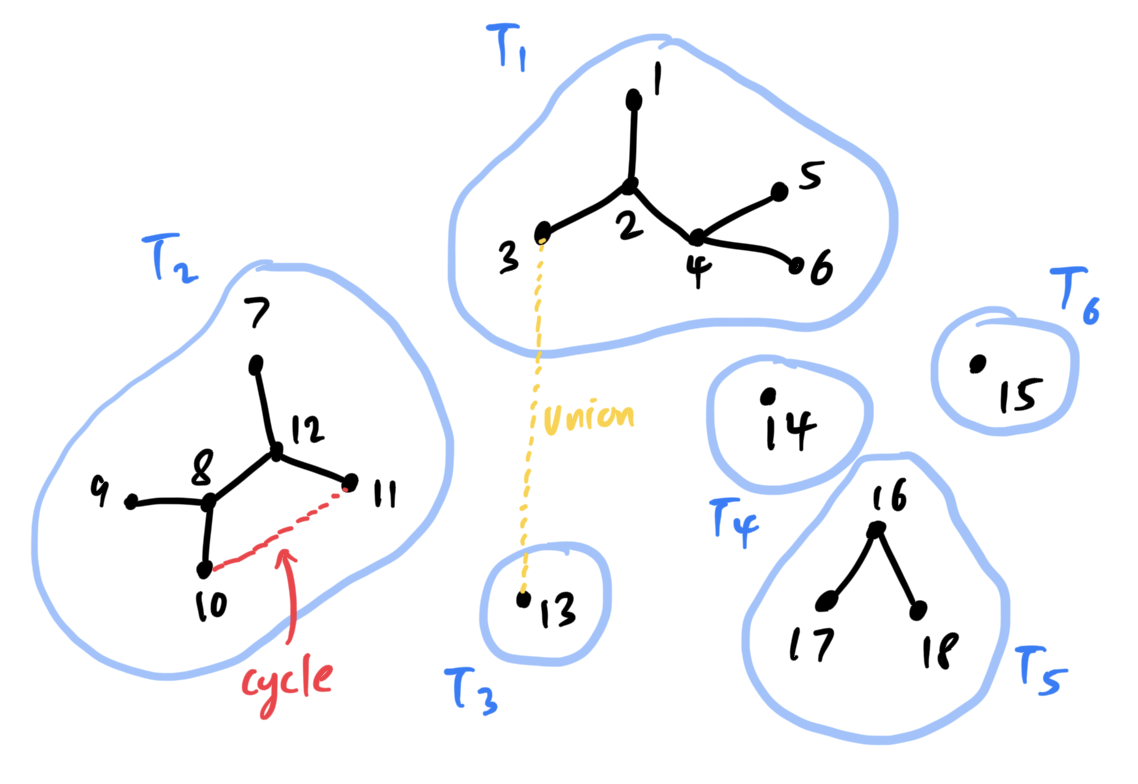
\includegraphics[scale=0.4]{img/sets.png}
      \caption{Each $T_i$ is a component formed by the edges chosen so far. For example, $T_1 = \{1, 2, 3, 4, 5, 6\}, \ldots$. We can either discard an edge (red) or include an edge (yellow). } 
      \label{fig:sets}
    \end{figure}

    The only bottleneck in here is line 5, where we check if $e$ does not complete a cycle in $T$. It will obviously not be efficient to do BFS, construct a tree, and see if there is a loop by checking if two points in the same layer are connected. It may help to decompose this algorithm into two steps: what is being stored and what is being checked? 

    Note that from our visual, we are really just keeping a set of these points that each make a subtree and connecting them together. How do we efficiently search for which cluster a point is a part of and efficiently merge two clusters? We could use a hashmap but this wouldn't work. We need something like a doubly linked list. 

    \begin{algo}[Kruskal's Algorithm]
      The implementation uses the Union-Find data structure. For clarity, we will not elaborate it but will show the full pseudocode. 
      \begin{algorithm}[H]
        \label{alg:kruskal}
        \begin{algorithmic}
          \Require{Nodes V. Edges $E = \{(u, v, w)\}$ where $u, v \in V$ and $w > 0$ is a weight. }
          \State 
          \Function{Kruskal}{V, E}
            \State $n \gets |V|$ 
            \State sort $E$ in increasing order of weights. \Comment{Needed for Kruskal}
            \State parent $\gets [0, \ldots, n-1]$ \Comment{Initialize the disjoint cluster each node is in}
            \State rank $\gets$ list of $0$s of size $n$ 

            \Function{Find}{x} 
              \If{parent[x] $\neq$ x} 
              \State parent[x] $\gets$ Find(parent[x]) \Comment{Path compression}
              \EndIf
              \State \Return{parent[x]}
            \EndFunction

            \Function{Union}{x, y} 
              \State px, py = find(x), find(y) 
              \If{px = py} 
                \State \Return{False}
              \EndIf
              \If{rank[px] < rank[py]} 
                \State parent[px] $\gets$ py
              \ElsIf{rank[px] > rank[py]}
                \State parent[py] $\gets$ px
              \Else{}
                \State parent[py] $\gets$ px 
                \State rank[px] $\gets$ rank[px] + 1
              \EndIf
              \State \Return{True}
            \EndFunction

            \State mst $\gets$ [] 
            \For{u, v, weight $\in$ edges} 
              \If{union(u, v)} 
                \State add (u, v, weight) to mst
              \EndIf 
              \If{len(mst) = n - 1}
                \State break
              \EndIf 
            \EndFor

            \State \Return{mst}
          \EndFunction
        \end{algorithmic}
      \end{algorithm}
    \end{algo}
    
    To analyze the runtime of this, we define the function. 

    \begin{definition}[Ackerman Function]
      The \textbf{Ackerman function} is one of the fastest growing functions known. It is practically infinity. 
      \begin{equation}
        A(m,n) = 
        \begin{cases} 
          n+1 & \text{if } m = 0 \\
          A(m-1,1) & \text{if } m > 0 \text{ and } n = 0 \\
          A(m-1,A(m,n-1)) & \text{if } m > 0 \text{ and } n > 0
        \end{cases} 
      \end{equation}
      The inverse Ackerman function therefore grows extremely slowly. 
    \end{definition}

    If we optimize the steps in Kruskal's algorithm, we can get its runtime to 
    \begin{equation}
      O((m + n) \log^{\ast} (n))
    \end{equation}
    which is practically linear. 

  \subsubsection{Applications}

    Here is a way to cluster data, a surprising way to apply MSTs. It is the most widely used application, especially in data science. The problem is that given $n$ data points $x_i \in \mathbb{R}^d$ and an integer $k$, we want to partition the points into $k$ groups $\mathbf{C} = (C_1, \ldots, C_k)$ where $\mathbf{x} = \sqcup_i C_i$. You want to distances between the points within a group to be small and the distances between groups to be large. We can think of finding the objective which takes every pair of clusters and computes the minimum distance between these clusters, and we want to maximize this distance over all pairs of clusters.  

    \begin{algo}[Single Linkage/Hierarchical Clustering]
      The general idea is to take this dense graph, find the MST, and cut off the largest edges from this MST, which will give you $k$ components. This is the answer. Or really, you can use Kruskal's algorithm and terminate earlier when $T$ has $k$ sets/components. 
      Note that as we add edges as we construct our MST, we are merging two clusters into one. So that all you are doing is finding the next pair of closest points and merging the clusters that they are a part of. 

      \begin{algorithm}[H]
        \label{alg:clustering}
        \begin{algorithmic}[1]
          \Require{Nodes $V = \{v_i\} \subset \mathbb{R}^n$}
          \Function{Cluster}{V}
            \State Run Kruskal and at each iteration, check if you have $K$ clusters. 
            \State If so, terminate and return the \texttt{parent} list. 
          \EndFunction
        \end{algorithmic}
      \end{algorithm}
    \end{algo}

    \begin{theorem}
      The algorithm above minimizes the objective function. 
      \begin{equation}
        \argmax_{\mathbf{C}} \min_{p \in C_i, q \in C_j} \{ d(p, q) \}
      \end{equation}
    \end{theorem}
    \begin{proof}
      Let $\mathbf{C}^\ast$ be the MST clustering. We claim that for any other clustering $\mathbf{C} = \{C_1, \ldots, C_k\}$,  
      \begin{equation}
        \mathrm{min dist}(\mathbf{C}) \leq \mathrm{min dist}(\mathbf{C}^{\ast})
      \end{equation}
      Assume that this was not the case, so $\mathrm{min dist}(\mathbf{C}) > \mathrm{min dist}(\mathbf{C}^{\ast})$ and therefore there exists a $p, q \in C_i, C_j$ such that $d(p, q) = \mathrm{mindist}(\mathbf{C}) > \mathrm{min dist}(\mathbf{C}^\ast)$. Since this is a different clustering, $p, q$ must have been in the same cluster $C_i^\ast$. But note that since Kruskal adds edges in increasing length, all edges within a cluster must have length less edges that go across two clusters. 

      \begin{figure}[H]
        \centering 
        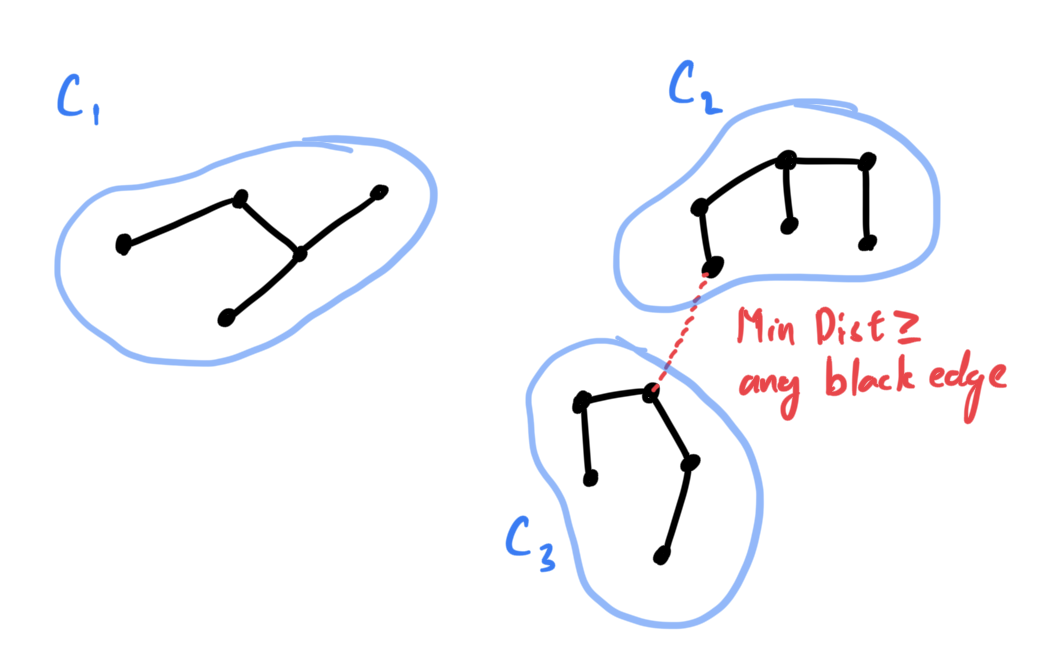
\includegraphics[scale=0.4]{img/mindist.png}
        \label{fig:mindist}
      \end{figure}

      So $d(p, q)$ must be the less than the length of all edges within a cluster in $\mathbf{C}^\ast$. But all within-cluster edges must be smaller than $\mathrm{min dist}(\mathbf{C}^\ast)$, meaning that $\mathrm{min dist}(\mathbf{C}^\ast) > d(p, q)$, contradicting the fact that is is greater, and we are done. 
    \end{proof}

    If you define the distance between two clusters to be the distance between the centroids (mean point), then this is called \textit{average linkage} (min avg distance). If we define the cluster distance as the maximum distance between two points, then it is called \textit{complete linkage} (min max distance). Kruskal's algorithm only worked for the single linkage case but may not work for these additional definitions. This is why there is usually a whole suite of clustering algorithms for a particular problem and we just find out which one fits the data the best. Furthermore, we have done \textit{bottom-up clustering}, where we took individual points to make clusters. In \textit{top-down clustering}, we take the whole set and cut it up into clusters.  


\section{Dynamic Programming}
  
  Let's take a look at a motivating example. 

  \begin{example}[Computing Fibonacci Numbers]
    To compute the $N$th Fibonacci number, we can use a recursive method. 
    \begin{algorithm}[H]
      \caption{}
      \label{alg:recfib}
      \begin{algorithmic}
        \Require{$N$}
        \State 
        \Function{RecFib}{$N$}
          \If{$N = 0$} 
            \State \Return{$0$}
          \ElsIf{$N = 1$}
            \State \Return{$1$}
          \Else 
            \State \Return{RecFib($N-1$) + RecFib($N-2$)}
          \EndIf
        \EndFunction
      \end{algorithmic}
    \end{algorithm}
  \end{example}

  This is exponential, in fact $O(\varphi^N)$ where $\varphi$ is the golden ratio. The reason is that we are repeatedly computing the same subproblem (e.g. RecFib($N-2$ is computed twice)), leading to inefficiency. It would be great if we could store these intermediate values rather than recomputing them. This introduces us to the concept of memoization. 

  \begin{definition}[Memoization]
    \textbf{Memoization} refers to storing intermediate values for reuse rather than computing them again (e.g. in future recursive calls). 
    
    Therefore, the term \textbf{dynamic programming} just means \textit{to deliberately evaluate and memoize in the correct order}. 
  \end{definition}


  \begin{algo}[Redursive Memoized Fibonacci]
    This leads us to a memoized version of computing Fibonacci Numbers, which is linear runtime. In fact, we can have constant space complexity since we don't need more than the last 2 previous Fibonacci numbers to compute the next one. 
    
    \begin{algorithm}[H]
      \caption{Memoized Fibonacci}
      \label{alg:memfib_rec}
      \begin{algorithmic}
        \Require{$N$}
        \State Initialize memo array $F[0..N]$ with -1
        \State $F[0] \gets 0$
        \State $F[1] \gets 1$
        \Function{MemFib}{$N$}
          \If{$N < 0$}
            \State \Return{$0$}
          \ElsIf{$F[N] \neq -1$}
            \State \Return{$F[N]$}
          \Else
            \State $F[N] \gets$ \Call{MemFib}{$N-1$} + \Call{MemFib}{$N-2$}
            \State \Return{$F[N]$}
          \EndIf
        \EndFunction
      \end{algorithmic}
    \end{algorithm}

    The runtime is computed, by taking the number of distinct problems (i.e. the number of calls to MemFib with distinct inputs) multiplied by the time per subproblem (constant since lookup is constant and adding is constant). Note that this assumes that arbitrary arithmetic operations take constant time, but this is not true if we look at the bit complexity, which can scale quite fast as these numbers grow. 
  \end{algo}

  Note that this does not really explicitly show the order in which the memoized list is being filled. It is implicit but hard to see in the recursive calls. Therefore, it may help to write it iteratively. 


  \begin{algo}[Iterative Memoized Fibonacci]
    In here, we can explicitly see that the $n$th Fibonacci number is explicitly dependent on the $n-2$ and $n-1$. 
    \begin{algorithm}[H]
      \caption{Iterative Fibonacci}
      \label{alg:iterfib}
      \begin{algorithmic}
        \Require{$N$}
        \State Initialize array $F[0..N]$
        \State $F[0] \gets 0$
        \State $F[1] \gets 1$
        \For{$i \gets 2$ to $N$}
          \State $F[i] \gets F[i-1] + F[i-2]$
        \EndFor
        \State \Return{$F[N]$}
      \end{algorithmic}
    \end{algorithm}
  \end{algo}

\subsection{Longest Increasing Subsequence}

  \begin{definition}[Longest Increasing Subsequence]
    Given a sequence of numbers $A = \{a_1, a_2, ..., a_n\}$, a \textbf{longest increasing subsequence} is a subsequence $\{a_{i_1}, a_{i_2}, ..., a_{i_k}\}$ of $A$ such that:
    \begin{enumerate}
      \item $1 \leq i_1 < i_2 < ... < i_k \leq n$ (maintains original order)
      \item $a_{i_1} < a_{i_2} < ... < a_{i_k}$ (strictly increasing)
      \item $k$ is maximized (longest such subsequence)
    \end{enumerate}
  \end{definition}

  \begin{example}
    For the sequence $A = \{3, 10, 2, 1, 20, 4, 25\}$:
    \begin{itemize}
      \item $\{3, 10, 20, 25\}$ is an increasing subsequence of length 4
      \item $\{2, 4, 25\}$ is an increasing subsequence of length 3
      \item $\{3, 10, 20, 25\}$ is a longest increasing subsequence as no increasing subsequence of length 5 or greater exists
    \end{itemize}
  \end{example}

  For the actual problem of calculating the length of the LIS, dynamic programming gives us an efficient approach. First, let's do a brute force algorithm. 

  \begin{algo}[Recursive Brute Force LIS]
    At each step, we consider whether to include the current element in our subsequence. We can only include it if it's larger than the previous element we chose, maintaining the increasing property. We explore both possibilities (including and excluding) recursively to find the longest possible subsequence.
    \begin{algorithm}[H]
      \caption{Recursive Brute Force Longest Increasing Subsequence}
      \label{alg:reclis}
      \begin{algorithmic}
        \Require{Array $A[1..n]$}
        \Function{LIS}{$A, i, prev$}  \Comment{$i$ is current position, $prev$ is last element we took}
          \If{$i = n + 1$}  \Comment{If we've processed all elements}
            \State \Return{$0$}  \Comment{Return 0 as we can't add more elements}
          \EndIf

          \State // First choice: skip current element
          \State skip $\gets$ \Call{LIS}{$A, i+1, prev$}  \Comment{Keep same prev, move to next element}

          \State // Second choice: try to take current element
          \State take $\gets 0$  \Comment{Initialize take option to 0 in case we can't take it}
          \If{$A[i] > prev$}  \Comment{Only if current element maintains increasing sequence}
            \State take $\gets 1 +$ \Call{LIS}{$A, i+1, A[i]$}  \Comment{Add 1 for taking current element}
          \EndIf \Comment{Recursively find best sequence starting at i+1 with A[i] as previous}

          \State // Return best option between taking and skipping
          \State \Return{max(skip, take)}  \Comment{Choose the better of our two options}
        \EndFunction
        
        \State // Initial call with sentinel value to allow taking any first element
        \State \Return{\Call{LIS}{$A, 1, -\infty$}}  \Comment{Start at first element, no previous restrictions}
      \end{algorithmic}
    \end{algorithm}
    The runtime can be used by the recurrence relation. At every call, we may at most have to compute $2$ calls on the subarray not including the current element, and we compute the max of them which takes $O(1)$, so 
    \begin{equation}
      T(N) = 2 T(N-1) + O(1) \implies T(N) = O(2^N)
    \end{equation}
    which is not good. 
  \end{algo}

  Now let's move to our DP solution. 

  \begin{algo}[Dynamic Programming LIS]
    The key insight is that LIS[i] (the length of the LIS within the input array ending at i, inclusive) depends on all previous LIS[j] where j < i and A[j] < A[i]. For each position i, we can extend any previous increasing subsequence that ends with a smaller value. In other words, we are solving 
    \begin{equation}
      \mathrm{LIS}[i] = 1 + \max\{\mathrm{LIS}[j] \mid j < i \text{ and } A[i] > A[j] \}
    \end{equation}

    \begin{algorithm}[H]
      \caption{Dynamic Programming Longest Increasing Subsequence}
      \label{alg:dplis}
      \begin{algorithmic}
        \Require{Array $A[1..n]$}
        \Function{DPLIS}{$A$}
          \State // Initialize LIS array - each single element is an increasing sequence
          \State Initialize array $LIS[1..n]$ with $1$  \Comment{Base case: each element forms LIS of length 1}
          
          \For{$i \gets 2$ to $n$}  \Comment{Consider each element as end of sequence}
            \For{$j \gets 1$ to $i-1$}  \Comment{Look at all previous elements}
              \If{$A[i] > A[j]$}  \Comment{Can we extend sequence ending at j?}
                \State $LIS[i] \gets \max(LIS[i], LIS[j] + 1)$  \Comment{Take best possible extension}
              \EndIf
            \EndFor
          \EndFor
          
          \State \Return{LIS[-1]} \Comment{Find the maximum value in LIS array}
        \EndFunction
      \end{algorithmic}
    \end{algorithm}

    The runtime is $O(n^2)$ since we have two nested loops, and the space complexity is $O(n)$ since we store one value for each position in the array. Note that we could also have filled this DP array backwards by considering all arrays that start at $A[i]$. 
  \end{algo}

  \begin{example}[DPLIS for Small Array]
    For array $A = [3,1,4,1,5]$:
    \begin{itemize}
      \item Initially: $LIS = [1,1,1,1,1]$
      \item After processing $i=2$: $LIS = [1,1,1,1,1]$
      \item After $i=3$: $LIS = [1,1,2,1,1]$ (4 can extend sequence from 3)
      \item After $i=4$: $LIS = [1,1,2,2,1]$
      \item After $i=5$: $LIS = [1,1,2,2,3]$ (5 can extend sequence from 4)
    \end{itemize}
    Final answer is 3, corresponding to subsequence $[3,4,5]$
  \end{example}

\subsection{0/1 Knapsack} 

  Another application of DP is in the following problem. 

  \begin{definition}[0/1 Knapsack]
    Given a knapsack with maximum weight capacity $W$, along with a set of $n$ items, each with:
    \begin{itemize}
      \item Weight/Cost $c_i$
      \item Value $v_i$
    \end{itemize}
    You want to know the size of the subset of items that maximizes total value while keeping total weight/Cost $\leq W$. The constraint is that each item can be picked at most once (hence 0/1). 
  \end{definition}

  \begin{example}
    For $n = 3$ items and capacity $W = 4$:
    \begin{itemize}
      \item Item 1: $(c_1 = 2, v_1 = 3)$
      \item Item 2: $(c_2 = 1, v_2 = 2)$
      \item Item 3: $(c_3 = 3, v_3 = 4)$
    \end{itemize}
    Optimal solution: Take items 1 and 2
    \begin{itemize}
      \item Total weight: $2 + 1 = 3 \leq 4$
      \item Total value: $3 + 2 = 5$ (maximum possible)
    \end{itemize}
  \end{example}

  The most natural way to approach this would be greedy, but this does not exactly work. 

  \begin{example}[Counter-Example for Greedy Knapsack]
    Let's consider a knapsack with capacity $W = 10$ and:
    \begin{itemize}
      \item Values $V = [100, 48, 60, 11]$
      \item Weights $C = [10, 6, 4, 1]$
    \end{itemize}
    Then the value/weight ratios would be 
    \begin{equation}
      V/C = [10, 8, 15, 11]
    \end{equation}
    and so we would choose to gain 60 for cost 4, then gain 11 for cost of 1. We do not have enough to buy any more and have a cost of 71, when we could have gotten a cost of 108 by buying 60 and 48 for a total of 10. 
  \end{example}

  Just like as always, we just solve this using recursive brute force and then apply optimization with DP. 

  \begin{algo}[Recursive Brute Force Knapsack]
    The key idea is that for each item, we have two choices: either include it (if we have enough capacity) or exclude it. We try both possibilities recursively to find the maximum value possible. In here, $i$ represents the current item we're considering and $r$ is the remaining weight we can still use. 
    \begin{algorithm}[H]
      \caption{Recursive Knapsack}
      \label{alg:recknapG}
      \begin{algorithmic}
        \Require{Values $V[1..n]$, Weights $W[1..n]$, Capacity $C$}
        \State V, W
        \Function{Knapsack}{$i, r$}  
          \If{$i = n + 1$ or $r = 0$}  \Comment{Base case}
            \State \Return{$0$}   \Comment{Either we've considered all items or filled the knapsack}
          \EndIf \Comment{No more value can be added}

          \State skip $\gets$ \Call{Knapsack}{$i+1, r$}  \Comment{1st Op: Skip current item and maintain same $r$}

          \State take $\gets 0$  \Comment{2nd Op: Try to include curr item}
          \If{$W[i] \leq r$}  \Comment{Only try taking if item's weight fits in remaining $r$}
            \State take $\gets V[i] +$ \Call{Knapsack}{$i+1, r - W[i]$} \Comment{Add current item's value + best value from remaining items}
          \EndIf \Comment{Subtract current item's weight from remaining $r$}

          \State \Return{$\max(take,skip)$} \Comment{Return best possible value between two choices}
        \EndFunction
        
        \State // Start considering from first item with full $r$ 
        \State \Return{\Call{Knapsack}{$1, C$}}
      \end{algorithmic}
    \end{algorithm}
  \end{algo}

  Now let's apply memoization. 

  \begin{algo}[Dynamic Programming Knapsack]
    The key insight is that $K[i,r]$ (best value possible using items up to i exclusive with remaining capacity r) can be built from $K[i-1,r]$ and $K[i-1,r-W[i]]$ using the formula 
    \begin{equation}
      K[i,r] = \begin{cases}
        K[i-1,r] & \text{if } W[i] > r \text{ (can't take item i)} \\
        \max(K[i-1,r], V[i] + K[i-1,r-W[i]]) & \text{if } W[i] \leq r \text{ (can take item i)}
      \end{cases}        
    \end{equation}
    In here, i represents the items 1..i we're considering and r represents the remaining capacity.
    \begin{algorithm}[H]
      \caption{Dynamic Programming Knapsack}
      \label{alg:dpknap}
      \begin{algorithmic}
        \Require{Values $V[1..n]$, Weights $W[1..n]$, Capacity $C$}
        \State V, W
        \Function{DPKnapsack}{$C$}
          \State Create table $K[0..n, 0..C]$ \Comment{K[i,r] = max value using items V[:i] with remaining r}
          \State Initialize all entries to 0
          
          \For{$i \gets 1$ to $n$}  \Comment{Consider each item}
            \For{$r \gets 0$ to $C$}  \Comment{Consider each possible remaining capacity}
              \State $K[i,r] \gets K[i-1,r]$  \Comment{Default: inherit value from excluding item i}
              \If{$r \geq W[i]$}  \Comment{If current item fits in remaining capacity}
                \State take $\gets V[i] + K[i-1,r-W[i]]$  \Comment{Value of item i + best value with remaining r}
                \State $K[i,r] \gets \max(K[i,r],$ take$)$  \Comment{Take better of including or excluding}
              \EndIf
            \EndFor
          \EndFor
          
          \State \Return{$K[n,C]$}  \Comment{Best value possible using all items}
        \EndFunction
      \end{algorithmic}
    \end{algorithm}
    The memory complexity is obviously $\Theta(n C)$. The number of subproblems is $nC$, and the processing for each step is constant time (possibly addition and max), so $O(1)$. Therefore the total runtime is $O(nC)$ also. Note that if we compare this in terms of the bit runtime, then this is $O(n \log_2 C)$, which is psuedopolynomial since $C$ is described by $\log_2 {C}$ bits. However, the $n$ will scale linearly since it is the size of the array and not the size of each integer in $V, W$. 
  \end{algo}

  Note that if $C$ can be very big, and this can be problematic. 

\subsection{Line Breaking}

  \begin{definition}[Line Breaking]
    Line breaking is used whenever you compile a tex document. Given 
    \begin{itemize}
      \item a sequence of words $w_1, w_2, ..., w_n$ where $w_i$ has length $l_i$
      \item a maximum line length $L$
      \item each line must contain whole words in order, separated by spaces
    \end{itemize}
    Our goal is to break words into lines to minimize the sum of squares of empty spaces at the end of each line, i.e. our cost function for a sequence of words $W[i:j+1]$ is 
    \begin{equation}
      \bigg( L - \sum_{k=i}^j w_k \bigg)^2
    \end{equation} 
    If we used the absolute value, there exists a greedy solution. 
  \end{definition}

  \begin{example}[Line Breaking Example]
    Given $L = 20$ and $W = [12, 8, 9]$ (note that spaces won't count in length in this problem), we have 3 possible arrangements. 
    \begin{enumerate}
      \item Option 1: First two words on first line
      \begin{itemize}
        \item Line 1: [12 + 8 = 20] (0 spaces remain)
        \item Line 2: [9] (11 spaces remain)
        \item Total cost = $0^2 + 11^2 = 121$
      \end{itemize}

      \item Option 2: Words one per line
      \begin{itemize}
        \item Line 1: [12] (8 spaces remain)
        \item Line 2: [8] (12 spaces remain)
        \item Line 3: [9] (11 spaces remain)
        \item Total cost = $8^2 + 12^2 + 11^2 = 64 + 144 + 121 = 329$
      \end{itemize}

      \item Option 3: Word 2 and 3 together
      \begin{itemize}
        \item Line 1: [12] (8 spaces remain)
        \item Line 2: [8 + 9 = 17] (3 spaces remain)
        \item Total cost = $8^2 + 3^2 = 64 + 9 = 73$
      \end{itemize}
    \end{enumerate}
    Therefore, Option 3 is optimal with cost 73. This also demonstrates that the greedy strategy, which gives Option 1, will not work. 
  \end{example}

  We start off with recursive brute force. Given any word $w_i$, we can either end the line there $w_i |$ or add another word $w_i w_{i+1}$. 

  \begin{algo}[Recursive Brute Force Line Breaking]
    The key idea is at each position i, we try placing different numbers of words on the current line and recursively solve for the rest. For each word i, we try all possible ways to break the line starting at word i. Let $MinCost(i)$ be the minimum cost to arrange words $[i..n]$. Then:
    \begin{equation}
      MinCost(i) = 
      \begin{cases}
        0 & \text{if } i > n \\
        \min_{i \leq j \leq n} \big\{ (L - \sum_{k=i}^j W[k])^2 + MinCost(j+1) \big\} & \text{if else} 
      \end{cases}
    \end{equation}
    where $(L - \sum_{k=i}^j W[k])^2$ is the cost to put the words $i...j$ on a new line and then ending. So whenever we add the new $i$th word at the end of the line, we are looking at all words $j$ at which we can break the line, and taking the minimum cost given this line break. The line break from $j+1$ should be computed as well (this is what we will store in our DP array later). 

    \begin{algorithm}[H]
      \caption{Recursive Line Breaking}
      \label{alg:recline}
      \begin{algorithmic}
        \Require{Word lengths $W[1..n]$, Line length $L$}
        \State W
        \Function{MinCost}{$i$}  \Comment{Returns min cost for words[i..n]}
          \If{$i = n + 1$}  \Comment{Base case: no words left}
            \State \Return{$0$}
          \EndIf

          \State min\_cost $\gets \infty$
          \State lineLen $\gets 0$
          \For{$j \gets i$ to $n$}  \Comment{Try placing words i through j on current line}
            \State lineLen $\gets$ lineLen $+ W[j]$
            \If{lineLen $\leq L$}  \Comment{If these words fit on the line}
              \State spaces $\gets L -$ lineLen  \Comment{Extra spaces at end of line}
              \State cost $\gets$ spaces$^2 +$ \Call{MinCost}{$j+1$}  \Comment{Cost of this line + rest}
              \State min\_cost $\gets \min($min\_cost$,$ cost$)$
            \EndIf
          \EndFor
          \State \Return{min\_cost}
        \EndFunction
        
        \State \Return{\Call{MinCost}{$1$}}  \Comment{Start with first word}
      \end{algorithmic}
    \end{algorithm}
  \end{algo}

  \begin{example}[Recursive Brute Force Line Breaking]
    For example, with $L=20$ and $W=[12,8,9]$:
    \begin{itemize}
      \item At $i=1$: Try
        \begin{itemize}
          \item [12] alone (8 spaces) + solve for [8,9]
          \item [12,8] together (0 spaces) + solve for [9]
        \end{itemize}
      \item At $i=2$: Try
        \begin{itemize}
          \item [8] alone (12 spaces) + solve for [9]
          \item [8,9] together (3 spaces) + solve for []
        \end{itemize}
      \item At $i=3$: Try
        \begin{itemize}
          \item [9] alone (11 spaces) + solve for []
        \end{itemize}
    \end{itemize}
  \end{example}

  \begin{algo}[Dynamic Programming Line Breaking]
    The key insight is that $DP[i]$ represents the minimum cost of optimally arranging words $[i..n]$. For each word i, we try placing words $[i..j]$ on a line and add the cost of optimally arranging the remaining words $[j+1..n]$. We do the same logic but rather than computing it we just retreive it from the DP array. 

    \begin{equation}
      DP[i] = 
      \begin{cases}
        0 & \text{if } i > n \\
        \min_{i \leq j \leq n} \big\{ (L - \sum_{k=i}^j W[k])^2 + DP[j+1] \big\} & \text{if else} 
      \end{cases}
    \end{equation}


    \begin{algorithm}[H]
      \caption{Dynamic Programming Line Breaking}
      \label{alg:dpline}
      \begin{algorithmic}
        \Require{Word lengths $W[1..n]$, Line length $L$}
        \State W
        \Function{LineBreak}{$L$}
          \State Create array $DP[0..n]$ \Comment{DP[i] = min cost for words[i..n]}
          \State Initialize all entries to $\infty$
          \State $DP[n+1] \gets 0$ \Comment{Base case: no words left}
          
          \For{$i \gets n$ downto $1$}  \Comment{Consider each starting word}
            \State lineLen $\gets 0$
            \For{$j \gets i$ to $n$}  \Comment{Try placing words i through j on a line}
              \State lineLen $\gets$ lineLen $+ W[j]$
              \If{lineLen $\leq L$}  \Comment{If these words fit on the line}
                \State spaces $\gets L -$ lineLen \Comment{Extra spaces at end}
                \State cost $\gets$ spaces$^2 + DP[j+1]$ \Comment{Cost of this line + rest}
                \State $DP[i] \gets \min(DP[i],$ cost$)$ \Comment{Update if better}
              \EndIf
            \EndFor
          \EndFor
          
          \State \Return{$DP[1]$}  \Comment{Cost of optimally arranging all words}
        \EndFunction
      \end{algorithmic}
    \end{algorithm}

    The memory complexity is clearly $O(n)$. To add each element $i$, we must iterate over all the possible $j$'s, making this $O(n^2)$ total iterations. However, computing the cost is also $O(n)$, making the total runtime $O(n^3)$. However, if we also store another DP array \texttt{sums}, which can be computed in linear time and stores 
    \begin{equation}
      \texttt{sums}[i] = \sum_{k=i}^n w_k \implies \sum_{k=i}^{j}  = \sum_{k=i}^n w_k - a\sum_{k=j+1}^n w_k = \texttt{sums[i]} - \texttt{sums[j+1]}
    \end{equation}
    which can be accessed and computed in $O(1)$ time, bringing us down to $O(n^2)$. 
  \end{algo}

  \begin{example}[DP Line Breaking]
    For example, with $L=20$ and $W=[12,8,9]$:
    \begin{itemize}
      \item $DP[4] = 0$ (base case)
      \item $DP[3] = 11^2 = 121$ (only option for last word)
      \item $DP[2] = \min(12^2 + 121, 3^2) = \min(265, 9) = 9$ (alone or with word 3)
      \item $DP[1] = \min(8^2 + 9, 0^2 + 121) = \min(73, 121) = 73$ (alone or with word 2)
    \end{itemize}
  \end{example}

\subsection{Bellman Ford Revisited} 

  Recall the Bellman equations that we must solve using DP. That is, given some $s \in V$, 
  \begin{equation}
    d[v] = \min_w \{ d[w] + l_{wv} \}
  \end{equation}
  with $d[s] = 0$. Note that the problem was not well defined if there are negative cycles in the graph, since we can just loop an infinite number of times. However, we can modify the bellman equations to get a better sense. 

  \begin{theorem}[Modified Bellman Equations]
    For paths of length at most $i$ edges, the Bellman equations become:
    \begin{align}
      d(v,i) = \begin{cases} 
        0 & \text{ if } v = s \\
        \min\{d(v,i-1), \min_{(u, v) \in E} \{d(u,i-1) + w_{uv}\}\} & \text{ otherwise}
      \end{cases}
    \end{align}
    where $d(v,i)$ represents the shortest path from source $s$ to vertex $v$ using at most $i$ edges, and $w_{uv}$ represents the weight of edge $(u, v)$. Note that the inner minimum takes the minimum over all paths with the final edge connecting from some other node $u$ to target $v$, and the outer minimum compares this minimum path to what we already have to see if it's an improvement. 
  \end{theorem} 

  This indicates that we should use a 2D DP array to memoize. This allows you to have a more flexible representation in case there are negative cycles since we are also limiting the number of edges a path could have. 

  \begin{algo}[2D DP Bellman-Ford]
    The implementation of the modified equations gives us the following algorithm. 
    \begin{algorithm}[H]
      \label{alg:bellman_ford_leq}
      \begin{algorithmic}[1]
        \Require{Nodes $V$, Edges $E$, source $s$}
        \State $d \gets$ 2D array of size $|V| \times |V|$ initialized to $\infty$
        \State $d[s,0] \gets 0$ \Comment{Base case: Can reach source with 0 edges}
        
        \For{$i = 1, \ldots, n-1$}
          \For{$v \in V$}
            \State $d[v,i] \gets d[v,i-1]$ \Comment{Keep best path seen so far}
            \For{$(u,v) \in E$}
              \State $d[v,i] \gets \min(d[v,i], d[u,i-1] + l_{uv})$
            \EndFor
          \EndFor
        \EndFor
      \end{algorithmic}
    \end{algorithm}
    Note that this algorithm still has time complexity $O(nm)$ because the outer loop runs $n-1$ times and for each iteration, we examine each edge once. The space complexity is $O(n^2)$, and finally, note the important properties. 
    \begin{enumerate}
      \item \textit{Monotonicity}: For all vertices $v$ and indices $i$:
      \begin{equation}
        d(v,i) \leq d(v,i-1)
      \end{equation}
      This is because any path using $\leq (i-1)$ edges is also a valid path using $\leq i$ edges.

      \item \textit{Convergence}: The algorithm will stabilize after at most $n-1$ iterations since:
      \begin{itemize}
        \item Any shortest path without negative cycles can use at most $n-1$ edges
        \item Therefore, $d(v,n-1) = d(v,n)$ for all $v$ if no negative cycles exist
      \end{itemize}

      \item \textit{Negative Cycle Detection}: A negative cycle exists if and only if:
      \begin{equation}
        \exists v \in V : d(v,n) < d(v,n-1)
      \end{equation}
      This is because any improvement after $n-1$ edges must use a negative cycle.
    \end{enumerate}
  \end{algo}


\section{Probabilistic Algorithms} 

\subsection{Primality Testing}


\section{Efficiency} 
  
\subsection{Classification of Decision Problems}

  We have talked about \textit{optimization problems} that choose the best solution from a class of solutions. Now we will talk about \textit{decision problems}, which seek to prove or disprove the existence of a solution satisfying a certain property. 

  \begin{lemma}[Conversion between Optimization and Decision Problems]
    It turns out we can convert one into the other easily by rephrasing the problem. The following conversion will be used frequently.  
    \begin{enumerate}
      \item Given a problem $P$, we want to find a solution that minimizes some variable $K$. 
      \item Given a problem $P$ and some constant $K^\prime$, does there exist a solution that is less than $K^\prime$? 
    \end{enumerate}
    Voila.  
  \end{lemma}

  Now that this is established, we can freely consider the classes P and NP of all decision problems and classify them. There are equivalent definitions for optimization problems, but it is more popular to pose these classes as decision problems. 

  \begin{definition}[P]
    $P$ (Polynomial Time) is the set of all decision problems that can be solved by polynomial-time algorithms. 
  \end{definition} 

  \begin{definition}[NP]
    $NP$ (Nondeterministic Polynomial Time) is the set of all decision problems for which if it returns $1$ (i.e. a solution exists), this can be \textit{verified} in polynomial time.\footnote{The fact that a \textit{proposed} solution can be verified is important! Proving or disproving a proposed solution is much easier than proving the nonexistence of a solution.}
  \end{definition}

  The other way around $NP \subset P$ is an unsolved millenium conjecture. It attempts to answer what the runtime difference or difficulty is between solving and verifying a problem? The conjecture states that solving is exponentially harder that verifying. 

  \begin{theorem}
    $P \subset NP$
  \end{theorem}
  \begin{proof}
    Given a problem $\pi$ with a proposed solution $p$, we can run $p$ in polynomial time to verify it. 
  \end{proof}

  Colloquially, the set of problems which are at least as hard as NP is called \textit{NP-hard}, which can be defined for both optimization and decision problems. These are the absolute hardest problems. The formal definition of NP-Hard problems is shown below. 

  \begin{definition}[NP-Hard]
    A (decision or optimization) problem $\pi$ is NP-hard iff the existence of a polynomial time algorithm for $\pi$ implies $P = NP$. 
  \end{definition}

  \begin{definition}[NP-Complete]
    The intersection of NP-hard and NP is \textbf{NP-complete}, which can be thought of as the hardest problems existing in NP. The worst case runtime complexity of an NP-complete problem is exponential. 
  \end{definition}

  \begin{figure}[H]
    \centering 
    \begin{tikzpicture}[scale=0.7]
      % Define styles for the ellipses
      \tikzset{
        complexity/.style={
          draw,
          thick,
          ellipse,
          minimum width=4cm,
          minimum height=2.5cm,
          font=\large\bfseries
        }
      }
      
      % Draw the complexity classes
      % NP-Hard at the top
      \draw[thick] (0,4) ellipse (4cm and 3cm);
      \node at (0,5) {\large\textbf{NP-Hard}};
      
      % NP in the middle
      \draw[thick] (0,0) ellipse (4cm and 3cm);
      \node at (0,0.25) {\large\textbf{NP}};
      
      % P at the bottom
      \draw[thick] (0,-1.5) ellipse (1.5cm and 1cm);
      \node at (0,-1.5) {\large\textbf{P}};
      
      % NP-Complete as the intersection of NP-Hard and NP
      \node at (0,2) {\large\textbf{NP-Complete}};
      
      % Complexity arrow
      \draw[->, ultra thick] (4.5,-2) -- (4.5,5);
      \node[rotate=90, font=\Large] at (5.2,1.5) {\textbf{Complexity}};
    \end{tikzpicture}
    \caption{Diagram of the 4 classes. The complexity rises as we go up. } 
    \label{fig:class}
  \end{figure}
  
\subsection{Proving NP-Hardness}

  To show that a problem is in P, all we have to do is find a polynomial time algorithm, which is what we've been doing this entire course. To show whether a problem is NP, we should show that it is verifiable in polynomial time, which we have also done so far. Proving NP-hardness (which then allows us to prove NP-completeness) is a bit more tricky. The pattern is always three things. 
  \begin{enumerate}
    \item \textit{Reduction}. Describe a polynomial time algorithm $f$ to transform an \textit{arbitrary instance} $x$ of a problem $\beta$ into a \textit{special instance} $y = f(x)$ of a problem $\pi$. 
    \item \textit{Equivalence}. Prove that if arbitrary $x$ is a true instance of $\pi$, then $y$ is a true instance of $\pi$. 
    \item \textit{Equivalence}. Prove that if arbitrary $y$ is a true instance of $\pi$, then $x$ is a true instance of $\pi$.\footnote{This is the hard part.} 
  \end{enumerate}

  \begin{definition}[Reduction]
    In other words, to prove a problem $\pi$ is NP-hard, reduce\footnote{The fact that we say reduce here is misleading, since we are showing that the reduction is at least as hard as the original.} a known NP-hard problem $\beta$ to $\pi$ in polynomial time (not the other way around!). If this reduction is possible, then we claim that $\pi$ must be at least as hard as $\beta$: $\beta \leq_p \pi$. 
    \begin{enumerate}
      \item Assume that we can solve $\pi$ in polytime. 
      \item Then we can solve $\beta$ in polytime by first converting any instance of $\beta$ to $\pi$ in polytime, and then polytime solving $\pi$.\footnote{In other words, there exists an injective (but not necessarily surjective) mapping from the set of solutions of $\pi$ to the set of solutions of $\beta$. }
      \item Therefore, $\pi \in P \implies \beta \in P$. 
    \end{enumerate}
    But since we already know $\beta$ is NP-hard, this creates a contradiction. Therefore, $\pi \not\in P$. 
  \end{definition}

  The reduction serves to compare the two problems, and the equivalence then serves to compare the set of solutions to these two problems.   

  \begin{definition}[Equivalence of Solutions]
    The next step is to show two things: 
    \begin{enumerate}
      \item A solution to $\pi$ implies a solution to $\beta$, and 
      \item A solution to $\beta$ implies a solution to $\pi$. 
    \end{enumerate}
  \end{definition} 

  As a general overview of popular problems and their relation to each other, we'll mention this now. 

  \begin{theorem}[Reduction Tree of NP-Hard Problems]
    For convenience. 
    \begin{enumerate}
      \item 3SAT is NP-hard by Cook-Levin 
      \item CircuitSAT is NP-hard by reducing from 3SAT 
      \item Max Independent Set is NP-hard by reducing from 3SAT 
      \item Min Vertex Cover is NP-hard by reducing from MIS 
      \item Max Clique is NP-hard by reducing from MIS \label{max-clique-np-hard}
      \item Hamiltonian Path is NP-hard 
      \item Hamiltonian Cycle is NP-hard by reducing from MVC, 3SAT, or Hamiltonian Path 
      \item Graph Coloring is NP-hard by reducing from 3SAT 
      \item Subset Sum is NP-hard by reducing from MVC 
      \item Planar CircuitSAT is NP-hard by reducing from CircuitSAT 
      \item Paritioning\footnote{Given a set $S$ of $n$ integers, are there disjoint subsets $A, B$ s.t. their sums are equal?} is NP-hard by reducing from Subset Sum. 
      \item Set Cover\footnote{Given a collection of sets $S$, find the smallest sub-collection of sets that contains all the elements in $\cup S$.} is NP-hard. 
      \item Longest Path is NP-hard. 
      \item MaxCut\footnote{Find the max cut of a graph.} is NP-hard. 
    \end{enumerate}
  \end{theorem}

\subsection{Logic and Satisfiability}

  \begin{definition}[CircuitSAT]
    Consider a black box circuit $f$, with input $\mathbf{x} \in \{0, 1\}^n$. We want to answer the question of whether there exists some $\mathbf{x}$ s.t. $f(\mathbf{x}) = 1$, i.e. whether the circuit is \textbf{satisfiable} (i.e. outputs a 1 bit). 

    \begin{figure}[H]
      \centering 
      \begin{tikzpicture}[scale=1.0]
        % Input labels
        \node (x1) at (0,3) {$x_1$};
        \node (x2) at (0,2) {$x_2$};
        \node (x3) at (0,1) {$x_3$};

        % NOT gate for x1
        \node[american not port, scale=0.7] (not1) at (2,3) {};

        % AND gate
        \node[american and port, scale=0.7] (and1) at (4,2.5) {};

        % OR gate
        \node[american or port, scale=0.7] (or1) at (6,1.5) {};

        % Final output
        \node (out) at (8,1.5) {$f(x_1,x_2,x_3)$};

        % Connections
        % x1 to NOT gate
        \draw (x1) -- (not1.in);
        
        % NOT output to AND input 1
        \draw (not1.out) -- ++(0.5,0) |- (and1.in 1);
        
        % x2 to AND input 2
        \draw (x2) -- ++(3,0) |- (and1.in 2);
        
        % AND output to OR input 1
        \draw (and1.out) -- ++(0.5,0) |- (or1.in 1);
        
        % x3 to OR input 2
        \draw (x3) -- ++(5,0) |- (or1.in 2);
        
        % OR output to final output
        \draw (or1.out) -- (out);

        % Gate reference symbols at bottom
        % AND gate reference
        \node[american and port, scale=0.7] (and-ref) at (2,-1) {};
        \node (and-x) at (1,-0.8) {$x$};
        \node (and-y) at (1,-1.2) {$y$};
        \node (and-out) at (3,-1) {$x \wedge y$};

        % OR gate reference
        \node[american or port, scale=0.7] (or-ref) at (5,-1) {};
        \node (or-x) at (4,-0.8) {$x$};
        \node (or-y) at (4,-1.2) {$y$};
        \node (or-out) at (6,-1) {$x \vee y$};

        % NOT gate reference
        \node[american not port, scale=0.7] (not-ref) at (8,-1) {};
        \node (not-x) at (7,-1) {$x$};
        \node (not-out) at (9,-1) {$\neg x$};

        % Connections for reference gates
        \draw (and-x) -- (and-ref.in 1);
        \draw (and-y) -- (and-ref.in 2);
        \draw (and-ref.out) -- (and-out);

        \draw (or-x) -- (or-ref.in 1);
        \draw (or-y) -- (or-ref.in 2);
        \draw (or-ref.out) -- (or-out);

        \draw (not-x) -- (not-ref.in);
        \draw (not-ref.out) -- (not-out);
      \end{tikzpicture}
      \caption{Some random circuit where $n = 5$.} 
      \label{fig:random_circuit}
    \end{figure}

    The obvious way is to brute force is an check all $2^n$ combinations, and this is the only way since this is black-box. However, even if we knew the circuit itself, the amount of computations that we need to solve this is conjectured to be still $O(2^n)$, though we may be able to cleverly shave off some calculations here and there.\footnote{It is not proven that there exists no exponential algorithm.}
  \end{definition}

  \begin{definition}[3SAT]
    Given a boolean formula $\phi$ of $N$ variables where each \textbf{clause} contains exactly 3 literals, determine if there exists a satisfying assignment to the variables that makes $\phi$ true. Formally:
    \begin{align*}
      \phi &= C_1 \land C_2 \land \cdots \land C_m \\
      C_i &= (l_{i1} \lor l_{i2} \lor l_{i3}) \\
      l_{ij} &\in \{x_k, \neg x_k\} \text{ for some } k \in \{1,\ldots,n\}
    \end{align*}
    where $x_k$ are boolean variables and $\neg x_k$ their negations. For example:
    \begin{align*}
      \phi = (x_1 \lor \neg x_2 \lor x_3) \land (\neg x_1 \lor x_2 \lor x_4) \land (x_2 \lor \neg x_3 \lor \neg x_4)
    \end{align*}
    Like CircuitSAT, this problem is also believed to require $O(2^n)$ time, and in fact these problems are polynomially reducible to each other (CircuitSAT $\leq_p$ 3SAT and 3SAT $\leq_p$ CircuitSAT). The key difference is that 3SAT has a very specific structure that makes it easier to analyze and reduce other problems to, making it a canonical NP-complete problem.\footnote{The restriction to exactly 3 literals per clause is not arbitrary - 2SAT is solvable in polynomial time, while 3SAT is NP-complete.}
  \end{definition}

  In fact, there is a polynomial time algorithm to translate between 3SAT and CircuitSAT, so the two are theoretically equivalent. 

  \begin{theorem}[P, NP Classification of SAT]
    For CircuitSAT, 
    \begin{equation}
      \texttt{CircuitSAT} \not\in P, \texttt{CircuitSAT} \in NP
    \end{equation}
    That is, it cannot be solved in polynomial time, but given a solution circuit and a satisfying assignment, the assignment can be verified in polynomial time. 
    For 3SAT, 
    \begin{equation}
      \texttt{3SAT} \not\in P, \texttt{3SAT} \in NP
    \end{equation}
    That is, it cannot be solved in polynomial time, but given a solution formula and a satisfying assignment, the assignment can be verified in $O(N^3)$ time ($N^3$ comes from the size of the expression). 
  \end{theorem}

  \begin{theorem}[Cook-Levin]
    3SAT is NP-complete. 
  \end{theorem} 
  \begin{proof}
    The proof is extremely long, and we use this as the initial point from which we start proving NP-hardness of other problems using reduction. 
  \end{proof}

  For example, to prove that CircuitSAT is NP-hard, we should reduce 3-SAT to CircuitSAT in polynomial time and then we are done. Reduction is quite complicated, so we omit this for now. 

\subsection{Graph Problems}

  \subsubsection{Maximum Independent Set}

    \begin{definition}[MIS]
      Given an undirected graph $G(V, E)$, an \textbf{independent set} is a subset $S \subseteq V$ such that no two vertices in $S$ are connected by an edge in $E$. The \textbf{maximum independent set} problem asks 
      \begin{enumerate}
        \item Given $G$, find an independent set of maximum cardinality. 
        \item Given $G$ and constant $K$, does there exist an independent set of size $\geq K$? 
      \end{enumerate}
    \end{definition}

    \begin{theorem}[Maximum Independent Set (MIS)]
      MIS is NP-hard.
    \end{theorem}
    \begin{proof}
      We prove NP-hardness by reducing from 3SAT, which is more structured than CircuitSAT. Given a 3SAT instance $\phi$, we construct a graph $G$ such that $\phi$ is satisfiable if and only if $G$ has an independent set of size $m$, where $m$ is the number of clauses in $\phi$. The reduction works as follows: For a 3SAT formula $\phi = C_1 \land C_2 \land \cdots \land C_m$ where each clause $C_i = (l_{i1} \lor l_{i2} \lor l_{i3})$, construct graph $G(V,E)$:

      \begin{enumerate}
        \item For each clause $C_i$, create a \textbf{clause gadget}: a triangle with vertices labeled $l_{i1}$, $l_{i2}$, and $l_{i3}$ with undirected edges between them. 
        \item Add \textbf{consistency edges}: for any two literals $l_{ij}$ and $l_{k\ell}$ from different triangles, add an edge if they are complementary (i.e., one is $x$ and the other is $\neg x$)
      \end{enumerate}

      This reduction has the following properties:
      \begin{itemize}
        \item Each triangle forces us to choose at most one literal from each clause
        \item Consistency edges ensure we can't choose contradictory literals
        \item Choosing $m$ vertices (one per triangle) corresponds to making each clause true
      \end{itemize}

      For equivalence, it turns out that $\phi$ is satisfiable iff the size of the IS in $G$ is exactly the number of clauses in $\phi$. 
      \begin{itemize}
        \item ($\Rightarrow$) If $\phi$ is satisfiable, choose one true literal from each clause to form an independent set of size $m$
        \item ($\Leftarrow$) If $G$ has an independent set of size $m$, it must contain exactly one vertex per triangle (by pigeonhole principle), giving us a valid satisfying assignment
      \end{itemize}

      Therefore, now that we have established the reduction, since 3SAT is NP-complete and we have a polynomial-time reduction to MIS, MIS is NP-hard.
    \end{proof}

    \begin{example}[3SAT Reduction of MIS]
      Consider the 3SAT formula 
      \begin{equation}
        \phi = (a \lor b \lor c) \land (b \lor \neg c \lor \neg d) \land (\neg a \lor c \lor d) \land (a \lor \neg b \lor \neg d)
      \end{equation}
      Following our reduction, we construct graph $G$ as follows:

      \begin{figure}[H] 
        \centering 
        \begin{tikzpicture}[scale=0.8]
          % Define styles for nodes
          \tikzset{
            regular node/.style={circle, draw, minimum size=0.7cm, inner sep=0pt},
            highlighted node/.style={circle, draw, fill=yellow!30, minimum size=0.8cm, inner sep=0pt, double},
          }
          
          % Position nodes in an octagonal arrangement
          % Top nodes
          \node[highlighted node] (a) at (0,4) {$a$};
          \node[regular node] (c1) at (2,4) {$c$};
          \node[regular node] (b1) at (1,3) {$b$};
          
          % Left side nodes
          \node[regular node] (bbar) at (-2,2) {$\bar{b}$};
          \node[highlighted node] (a2) at (-1,1) {$a$};
          \node[regular node] (dbar) at (-2,0) {$\bar{d}$};
          
          % Right side nodes
          \node[regular node] (b2) at (4,2) {$b$};
          \node[regular node] (cbar) at (3,1) {$\bar{c}$};
          \node[highlighted node] (dbar2) at (4,0) {$\bar{d}$};
          
          % Bottom nodes
          \node[regular node] (abar) at (0,-2) {$\bar{a}$};
          \node[highlighted node] (c2) at (2,-2) {$c$};
          \node[regular node] (d) at (1,-1) {$d$};
          
          % Draw black edges (regular connections)
          \draw (a) -- (b1);
          \draw (b1) -- (c1);
          \draw (a) -- (c1);

          \draw (bbar) -- (a2);
          \draw (a2) -- (dbar);
          \draw (bbar) -- (dbar);

          \draw (b2) -- (cbar);
          \draw (cbar) -- (dbar2);
          \draw (b2) -- (dbar2);

          \draw (abar) -- (c2);
          \draw (abar) -- (d);
          \draw (d) -- (c2);
          
          % Draw red edges (special connections)
          \draw[red, thick] (bbar) -- (b2);
          \draw[red, thick] (b1) -- (bbar);
          \draw[red, thick] (a) -- (abar);
          \draw[red, thick] (dbar) -- (d);
          \draw[red, thick] (dbar2) -- (d);
          \draw[red, thick] (c1) -- (cbar);
          \draw[red, thick] (c2) -- (cbar);
          \draw[red, thick] (a2) -- (abar);
        \end{tikzpicture}
        \caption{Reduction graph from 3SAT to MIS. } 
        \label{fig:mis_graph}
      \end{figure}

      The graph contains:
      \begin{enumerate}
        \item Four triangles, one for each clause of $\phi$
        \item Red edges connecting complementary literals (e.g., $b$ with $\bar{b}$)
        \item A maximum independent set highlighted in yellow ($\{a, d\}$) of size 4
      \end{enumerate} 

      This independent set corresponds to the satisfying assignment $(a, b, c, d) = (1, \ast, 1, 0)$. 
      \begin{itemize}
        \item $(a \lor b \lor c)$ is satisfied by $a = 1$
        \item $(b \lor \neg c \lor \neg d)$ is satisfied by $d = 0$. 
        \item $(\neg a \lor c \lor d)$ is satisfied by $c = 1$. 
        \item $(a \lor \neg b \lor \neg d)$ is satisfied by $a = 1$. 
      \end{itemize}

      To demonstrate the proof, we assume that this MIS can be solved in polynomial time, so $MIS \in P$. But since $3SAT \leq_p MIS$, this means that $3SAT \in P$, which is a contradiction since $3SAT \in NP-hard$. 
    \end{example} 

  \subsubsection{Minimum Vertex Cover}

    \begin{definition}[Min Vertex Cover]
      Given an undirected graph $G(V, E)$, a \textbf{vertex cover} is a subset $S \subset V$ where for all $(u, v) \in E$, either $u \in S$ or $v \in S$ (or both). The \textbf{minimum vertex cover} problem asks 
      \begin{enumerate}
        \item Given $G$, find a vertex cover of minimum cardinality. 
        \item Given $G$ and constant $K$, does there exist a vertex cover of size $\leq K$? 
      \end{enumerate}
    \end{definition}

    \begin{theorem}[MVC]
      MVC is NP-hard. 
    \end{theorem}
    \begin{proof}
      \textit{Reduction from MIS}. Recall that an independent set is a subset $S \subset V$ s.t. for all $(u, v) \in E$, $u \in S$ or $v \in S$ (but not both). By definition, we can see that $u \in S \iff u \not\in V \setminus S$, and so IS and VCs are related in the following way: 
      \begin{align}
        S \subset V \text{ is a VC} & \iff \forall (u, v) \in E, u \in S \text{ or } v \in S \text{ or both} \\
                                    & \iff \forall (u, v) \in E, u \not\in S \setminus V \text{ or } v \not\in S \setminus V \text{ or both} \\
                                    & \iff V \setminus S \text{ is an IS}
      \end{align}
      Therefore, if $S$ has size $K$, then $V \setminus S$ will have size $N - K$. We assume that a polytime algorithm exists for MVC, so on input $G(V, E)$, we calculate the MVC, call it $M$, and then we return the corresponding MIS $S = V \setminus M$. 

      \textit{Equivalence}. 
      \begin{enumerate}
        \item ($\Rightarrow$) Assuming we have the solution $|S|$ for MVC, we can return true iff $|V| - |S| \geq K$. 
        \item ($\Leftarrow$) Assuming we have the solution $|S|$ for MIS, we can return true iff $|V| - |S| \leq K$. 
      \end{enumerate}
      But this would imply that there exists such a polytime algorithm, implying that $P = NP$, and therefore MVC must be NP-hard by definition. 
    \end{proof}

    \begin{example}[Reduction from Independent Set to Vertex Cover]
      Just take the complement. 
    \end{example}

  \subsubsection{Maximum Clique}

    \begin{definition}[Max Clique]
      Given an undirected graph $G(V, E)$, a \textbf{clique} is a subset of vertices $S \subset V$ s.t. there is an edge between each pair in $S$, i.e. a \textit{complete subgraph}. The \textbf{maximum clique} problem asks 
      \begin{enumerate}
        \item Given $G$, find the clique of maximum cardinality. 
        \item Given $G$ and constant $K$, does there exist a vertex cover of size $\geq K$? 
      \end{enumerate}
    \end{definition} 

    \begin{theorem}[MC]
      Finding the max clique is NP-hard. 
    \end{theorem}
    \begin{proof}
      \textit{Reduction from MIS}. Observe that 

      Let's define the \textbf{edge-complement} of a graph $G$ as $\bar{G} = (V, \bar{E})$ where $\bar{E}$ is the set of edges not in $G$. Then, note that 
      \begin{align}
        S \subset V \text{ is an IS of } G & \iff \forall u, v \in S, (u, v) \not\in E  \\
                                           & \iff \forall u, v \in S, (u, v) \in \bar{E} \\
                                           & \iff S \text{ is a clique of } \bar{G} 
      \end{align}
      Therefore, we can reduce this from MIS by taking input $G$, getting $\bar{G}$ in $O(N + M)$ time, solving the MIS of $\bar{G}$, and returning the size of the max clique of $\bar{G}$ in our assumed polytime algorithm. Therefore, MC is NP-hard. In fact, we have already proved the equivalence at the same time due to the iff conditions, but we state it explicitly for completeness. 

      \textit{Equivalence}. 
      \begin{enumerate}
        \item ($\Rightarrow$) Assuming we have the MIS solution $S \subset G$, then $S$ is the max clique of $\bar{G}$. 
        \item ($\Leftarrow$) Assuming we have the max clique solution $S \subset G$, then $S$ is the MIS of $\bar{G}$. 
      \end{enumerate}
    \end{proof}

    \begin{example}[Reduction of Independent Set to Clique]
      Just take the edge complement. 
    \end{example}

  \subsubsection{Hamiltonian Paths} 

    \begin{definition}[Hamiltonian Path]
      A \textbf{Hamiltonian path} in a directed graph $G$ is a path that visits every vertex exactly once. 
    \end{definition} 

    \begin{theorem}
      Finding the existence of a Hamiltonian cycle of a graph $G$ is NP-hard. 
    \end{theorem}

    \begin{definition}[Hamiltonian Cycle]
      A \textbf{Hamiltonian cycle} in a directed graph $G$ is a cycle that visits every vertex exactly once. 
    \end{definition}

    \begin{theorem}
      Finding the existence of a Hamiltonian cycle of a graph $G$ is NP-hard. 
    \end{theorem}
    \begin{proof}
      \textit{Reduction from VC}. Given an undirected graph $G(V, E)$ and integer $K$, we want to construct a directed graph $H(V^\prime, E^\prime)$, such that $H$ has a Hamiltonian cycle iff $G$ has a vertex cover of size $K$. We construct $H$ in the following. 
      \begin{enumerate}
        \item For each undirected edge $(u, v) \in E$, the directed graph $H$ contains an \textit{edge gadget} containing 4 vertices 
          \begin{equation}
            (u, v, \mathrm{in}), (u, v, \mathrm{out}), (v, u, \mathrm{in}), (v, u, \mathrm{out})
          \end{equation}
          and 6 directed edges 
          \begin{align*}
            & (u, v, \mathrm{in}) \rightarrow (u, v, \mathrm{out}) & 
            & (u, v, \mathrm{in}) \rightarrow (v, u, \mathrm{in}) & 
            & (v, u, \mathrm{in}) \rightarrow (u, v, \mathrm{in}) \\
            & (v, u, \mathrm{in}) \rightarrow (v, u, \mathrm{out}) & 
            & (u, v, \mathrm{out}) \rightarrow (v, u, \mathrm{out}) & 
            & (v, u, \mathrm{out}) \rightarrow (u, v, \mathrm{out})
          \end{align*}

          \begin{figure}[H]
            \centering 
            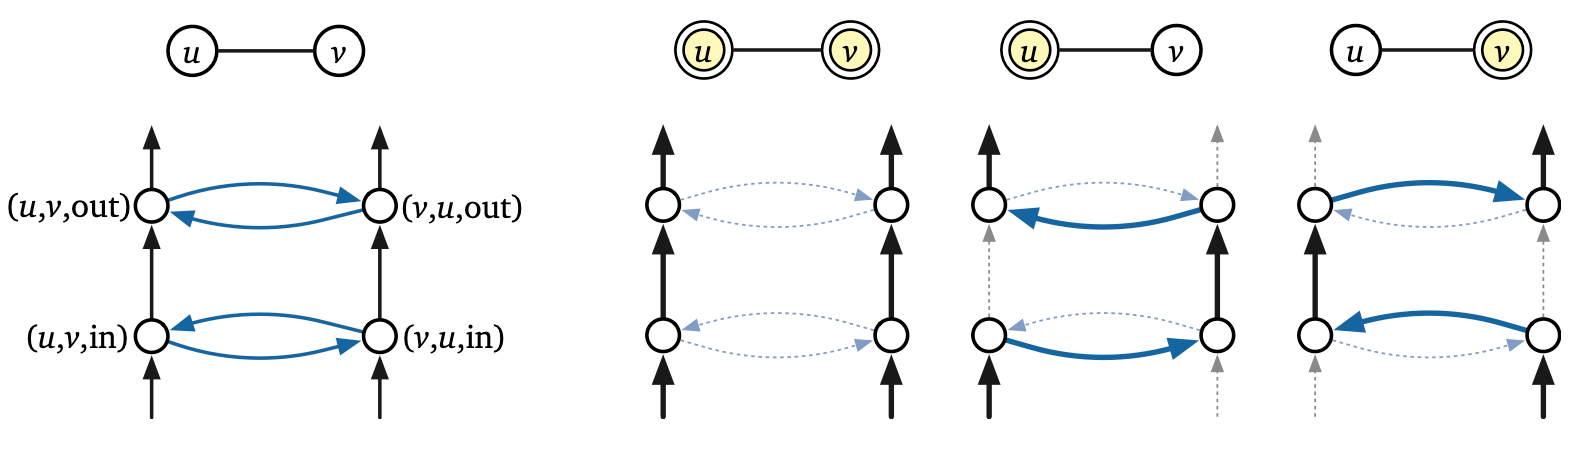
\includegraphics[scale=0.4]{img/edge_gadget.png}
            \caption{An edge gadget and its only possible interactions with a Hamiltonian cycle. Any Hamiltonian cycle in $H$ must pass through an edge gadget in one of 3 ways: straight through on both sides, or with a detour from one side to the other and back. These options will correspond to both $u$ and $v$, only $u$, or only $v$ belonging in the vertex cover.} 
            \label{fig:edge_gadget}
          \end{figure}

        \item For each vertex $u \in V$, all the edge gadgets for incident edges $(u, v)$ are connected in $H$ into a single directed path, called a \textit{vertex chain}. Specifically, suppose vertex $u$ has $d$ neighbors $v_1, \ldots, v_d$. Then $H$ has $d-1$ additional edges $(u, v_i, \mathrm{out}) \rightarrow (u, v_{i+1}, \mathrm{in})$ for each $i = 1, \ldots, d-1$.  

        \item Finally, $H$ also contains $k$ \textit{cover vertices} $x_1, \ldots, x_k$. Each cover vertex has a directed edge to the first vertex in the vertex chain, and a directed edge from the last vertex in each vertex chain. 
      \end{enumerate}

      \textit{Equivalence}. 
      \begin{enumerate}
        \item Suppose that $C = \{u_1, \ldots, u_k\}$ is a vertex cover of $G$ of size $k$. We can construct a Hamiltonian cycle that encodes $C$ as follows. 
        \item Suppose that $H$ contains a Hamiltonian cycle $C$. This cycle must contain an edge from each cover vertex to the start of some vertex chain. 
      \end{enumerate}
    \end{proof}

    \begin{example}[Reduction from Vertex Cover to Directed Hamiltonian Cycle]
      We can see that each double arrowed blue segment represents a pair of directed edges, each part of the gadget. 

      \begin{figure}[H]
        \centering 
        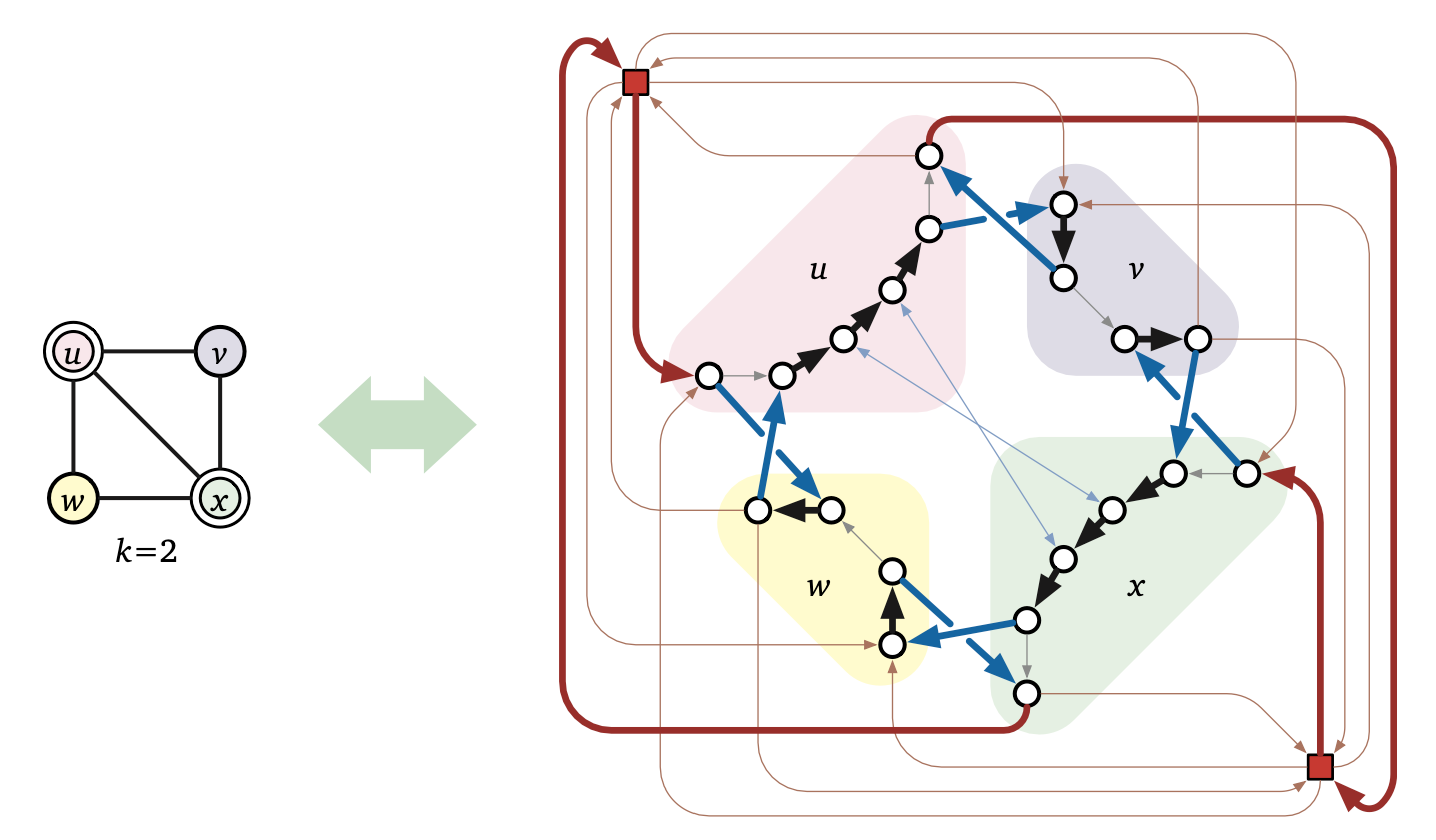
\includegraphics[scale=0.4]{img/ham_reduction.png}
        \caption{Reduction of a simple undirected graph to Hamiltonian cycle.} 
        \label{fig:ham_reduction}
      \end{figure}
    \end{example}

  \subsubsection{Euler Paths}

  \subsubsection{Longest Path}

    \begin{theorem}[Longest Path]
      Finding the longest path in a graph is NP-complete. 
    \end{theorem}

  \subsubsection{Graph Coloring} 

    \begin{definition}[Proper K-coloring]
      A \textbf{proper k-coloring} of a graph $G(V, E)$ is a function $C: V \rightarrow \{1, \ldots k\}$ that assigns one of $k$ colors to each vertex, so that every edge has two different colors at its endpoints. 
    \end{definition}

    \begin{theorem}
      Graph coloring is NP-hard. 
    \end{theorem}
    \begin{proof}
      \textit{Reduction from 3SAT}. 
    \end{proof}

\subsection{Subset Sum}

  \begin{definition}[Subset Sum]
    Given a multiset (allowing duplicates) $X$ of positive integers and a target value $T$, we want to find whether there exists a subset $S \subset X$ that sum up to $T$. 
  \end{definition}

  \begin{theorem}
    Finding the subset sum is NP-hard. 
  \end{theorem}
  \begin{proof}
    \textit{Reduction from MVC}. Given an arbitrary graph $G$ and integer $K$, we need to compute a set $X$ of positive integers and integer $T$, such that $X$ has a subset of sum $T$ iff $G$ has a vertex cover of size $K$. The general idea is that we label each edge with a number in $\{0, 1, 2, 3\}$, where $2$ means that the edge is in the vertex cover. 
    \begin{enumerate}
      \item We label each edge of $G$ from $e = 0, 1, \ldots, E-1$. 
      \item Construct $X = \{\}$: 
      \item for each $e = 0, \ldots, E-1$, add $b_e = 4^e$ to $X$. 
      \item for each vertex $v$, add 
      \begin{equation}
        a_v = 4^{E} + \sum_{e \in \Delta(v)} 4^e
      \end{equation}
      to $X$, where $\Delta(u)$ are the incident edges of $u$. What we have just done is represented each integer in $X$ as an $(E + 1)$ digit number written in base 4. The $E$th digit is $1$ if the integer represents a vertex and $0$ otherwise. For each $e < E$, the $e$th digit is $1$ if the integer represents edge $e$ or one of its endpoints, and $0$ otherwise. 

      \item We set our target sum to be 
      \begin{equation}
        T = K \cdot 4^E = \sum_{e=0}^{E-1} 2 \cdot 4^e
      \end{equation}
      where the first term covers all vertices and the summation covers all edges. 
    \end{enumerate}

    \textit{Equivalence}. 
    \begin{enumerate}
      \item Suppose $G$ has a vertex cover $C$ of size $k$. Consider the subset 
      \begin{equation}
        X^\prime = \{a_v \mid v \in C\} \cup \{b_e \mid \text{edge } e \text{ has exactly 1 endpoint in } C\} 
      \end{equation}
      The sum of the elements in $X^\prime$, written in base 4, has most significant digit $k$ and all other digits equal to $2$. Thus the elements of $X^\prime$ sum exactly to $T$. 

      \item Suppose that there is a subset $X^\prime \subset X$ that sums to $T$. We must have 
      \begin{equation}
        \sum_{v \in V^\prime} a_v + \sum_{e \in E^\prime} b_e = T
      \end{equation}
      for some subset $V^\prime \subset V, E^\prime \subset E$. Then each $b_e$ contributes exactly one digit of $1$ (in base 4). Each edge is incident to 2 vertices, so the non-significant digits contribute two digits of $1$. Therefore, if we sum these base-4 numbers, there are no carries in the first non-sigf $E$ digits since for each $e$ there are only 3 numbers in $X$ whose $e$th digit is $1$. Each edge number $b_e$ contribute only one 1 to the $e$th digit of the sum, but the $e$th digit of $T$ is $2$. Thus, for each edge in $G$, at least one of its endpoints must be in $V^\prime$. In other words, $V^\prime$ is a vertex cover. 
    \end{enumerate}

  \end{proof}

  \begin{example}[Reduction from Vertex Cover to Subset Sum] 
    Given the 4 vertex graph $G$ with $V = \{u, v, w, x\}$ and $E = \{uv, uw, vw, vx, wx\}$, our set $X$ will contain the following base-4 integers. 
    \begin{align*}
      a_u &:= 111000_4 = 1344 & b_{uv} &:= 010000_4 = 256 \\
      a_v &:= 110110_4 = 1300 & b_{uw} &:= 001000_4 = 64 \\
      a_w &:= 101101_4 = 1105 & b_{vw} &:= 000100_4 = 16 \\
      a_x &:= 100011_4 = 1029 & b_{vx} &:= 000010_4 = 4 \\
      & & b_{wx} &:= 000001_4 = 1
    \end{align*} 
    We can see that all the $a$'s have most significant digit $1$, meaning that it represents a vertex, and all the $b$'s that represent an edge are simply stored with a single $1$ and rest $0$s. For the $a$'s, the non-significant digits represent the incident edges. Vertex $u$ has connections to $v, w$, so the next 2 bits, representing the $1$ bits for edges $uv, uw$ are flipped to $1$. If we are looking for a vertex cover of size $K = 2$, we have 
    \begin{equation}
      T = 222222_4 = 2730
    \end{equation} 
    Indeed the vertex cover $\{v, w\}$ corresponds to the subset $\{a_v, a_w, b_{uv}, b_{uw}, b_{vx}, b_{wx}\}$, whose sum is $1300 + 1105 + 256 + 64 + 4 + 1 = 2730$. 
  \end{example}


\section{Streaming Algorithms}

\begin{algo}[Track Median From Data Stream]
  \begin{algorithm}[H]
    \caption{Track Median From Data Stream}
    \label{alg:median_track}
    \begin{algorithmic}[1]
      \Require{Stream of numbers} \Comment{Input is a continuous stream of numbers}
      \Ensure{Current median after each number} \Comment{Returns median as each number arrives}
      
      \State maxHeap $\gets$ empty max heap \Comment{Stores lower half of numbers}
      \State minHeap $\gets$ empty min heap \Comment{Stores upper half of numbers}
      
      \Function{AddNumber}{num}
        \If{maxHeap.isEmpty() OR num < maxHeap.peek()} \Comment{Number belongs in lower half}
          \State maxHeap.add(num) \Comment{Add to max heap}
        \Else
          \State minHeap.add(num) \Comment{Add to min heap}
        \EndIf
        
        \State balance $\gets$ maxHeap.size() - minHeap.size() \Comment{Check heap balance}
        
        \If{balance > 1} \Comment{Max heap has too many elements}
          \State minHeap.add(maxHeap.poll()) \Comment{Move largest from max heap to min heap}
        \ElsIf{balance < -1} \Comment{Min heap has too many elements}
          \State maxHeap.add(minHeap.poll()) \Comment{Move smallest from min heap to max heap}
        \EndIf
      \EndFunction
      
      \Function{FindMedian}{}
        \If{maxHeap.size() > minHeap.size()} \Comment{Odd number of elements}
          \State \Return maxHeap.peek() \Comment{Return top of max heap}
        \ElsIf{minHeap.size() > maxHeap.size()} \Comment{Odd number of elements}
          \State \Return minHeap.peek() \Comment{Return top of min heap}
        \Else \Comment{Even number of elements}
          \State \Return (maxHeap.peek() + minHeap.peek()) / 2 \Comment{Average of both tops}
        \EndIf
      \EndFunction
    \end{algorithmic}
  \end{algorithm}
\end{algo}


\section{Linear Programming}

  Basically, you want to solve a constrained optimization problem. Some examples are 
  \begin{enumerate}
    \item Shortest path: select a set of edges of minimum cost such that $s$ and $t$ are connected. 
    \item Minimum Spanning Tree: select a set of edges of minimum cost such that all vertices are connected. 
    \item Maximum Flow: select a flow on every edge such that capacity and balance constraints are respected. 
  \end{enumerate} 


  \begin{definition}[Linear Programming]
    In linear programming both the constraints and optimization objectives are linear functions. It is usually written in \textit{canonical form}, of the form 
    \begin{equation}
      \min c^T x \text{ subject to } Ax \geq b, x \geq 0
    \end{equation}
    or 
    \begin{equation}
      \max c^T x \text{ subject to } Ax \leq b, x \geq 0
    \end{equation}
    where we have $n$ variables $x \in \mathbb{R}^n$, $c \in \mathbb{R}^n$ are the optimization coefficients, and $A \in \mathbb{R}^{m \times n}$ are the matrix of $m$ constraint equations. 
  \end{definition} 

  \begin{example}[Simple LP]
    We can have the problem of maximizing $2x + y$ subject to 
    \begin{align}
      x + y & \leq 1 \\ 
      x & \geq 0  \\
      y & \geq 0
    \end{align}
    In this case, we can write it in canonical form as 
    \begin{equation}
      \max \begin{pmatrix} 2 & 1 \end{pmatrix} \begin{pmatrix} x \\ y \end{pmatrix} \text{ subject to } \begin{pmatrix} 1 & 1 \end{pmatrix} \begin{pmatrix} x \\ y \end{pmatrix} \leq 1, \begin{pmatrix} x \\ y \end{pmatrix} \geq \begin{pmatrix} 0 \\ 0 \end{pmatrix}
    \end{equation}
  \end{example}

  \begin{theorem}[Optimality of LP]
    An optimal solution to a linear program can be obtained in weakly polynomial time in the number of variables, constraints, and poly-logarithmic in the constants in the LP.\footnote{Obtaining a strongly polynomial algorithm for LPs remains a major open problem.} 
  \end{theorem} 

  This is very similar to integer programs, which solve for integer solutions rather than real, but in general we don't know of algorithms that can solve integer programs in polynomial time. However, integer programs can be ``relaxed'' to linear programs by removing the restriction on variables being integers. However, the optimal solution for the relaxed LP may be different from that of the original LP. 

  \begin{example}[Max Flow as LP]
    
  \end{example}

  \begin{example}[Bipartite Matching as LP]
    
  \end{example} 

  \begin{example}[Primal vs Dual LP]
    Now given a maximization LP problem, such as 
    \begin{equation}
      \max{2x + y} \text{ subject to } \begin{cases} x + y \leq 3 \\ x - y \leq 1 \\ x, y \geq 0 \end{cases} 
    \end{equation}
    we can just find \textit{one} solution satisfying the constraints and use it as a lower bound on the optimum. Say we find one, e.g. $x = y = 0$, which does satisfy all constraints. Now if we want to find an \textit{upper bound} on the value of the solution, we can use duality. We create new variables $a, b \geq 0$, and observe that 
    \begin{align}
      x + y \leq 3 & \implies a (x + y) \leq 3a \\
      x - y \leq 1 & \implies b (x - y) \leq b
    \end{align}
    Thus by adding the two we have $(a + b) x + (a - b) y \leq 3a + b$. 

    Now if we suppose $a + b \geq 2$ and $a - b \geq 1$ (which are the coeffients of $2x + y$), then since $x, y \geq 0$, we have 
    \begin{equation}
      2x + y \leq (a + b) x + (a - b) y \leq 3a + b
    \end{equation} 
    so any $a, b$ satisfying the above inequalities give an upper bound of $3a + b$ on the value of the optimal solution. Say we have $a = 2, b = 1$, which does satisfy. Then $3a + b = 7$ is an upper bound of $2x + y$. Therefore, to get the tightest upper bound, we can minimize the dual problem 
    \begin{equation}
      \min{3a + b} \text{ subject to } \begin{cases} a + b \geq 2 \\ a - b \geq 1 \\ a, b \geq 0 \end{cases}
    \end{equation}
    This is called the \textbf{dual LP}.
  \end{example}
  
  Generally, given the primal $\max{c^T x}$ subject to $Ax \leq b$ and $x \geq 0$, the dual problem is to compute $\min{b^T y}$ subject to $A^T y \geq c$ and $y \geq 0$. Every dual variable corresponds to a primal constraint and vice versa. If a primal has $n$ variables and $m$ constraints, the dual has $m$ variables and $n$ constraints. 

  \begin{theorem}
    The dual of a dual is the primal. 
  \end{theorem}

  \begin{theorem}[Weak Duality]
    The following properties are called \textbf{weak duality}. 
    \begin{enumerate}
      \item The optimal value for a dual maximization LP is a lower bound on the optimal value for a primal minimization LP. 
      \item The optimal value for a dual minimization LP is an upper bound on the optimal value for a primal maximization LP. 
    \end{enumerate}
  \end{theorem}

  \begin{theorem}[Strong Duality]
    The optimal value of a primal and dual LP are exactly identical, called \textbf{strong duality}. 
  \end{theorem}

\end{document}
